% ============================================================
% Training-Free Cultural Alignment of Large Language Models
% via Persona Disagreement  (method name: DISCA)
% NeurIPS 2026 Submission
% Compile: pdflatex -> bibtex -> pdflatex -> pdflatex
% ============================================================
\documentclass{article}
\usepackage{neurips_2026}  %\usepackage[main]{neurips_2026}

\usepackage[utf8]{inputenc}
\usepackage[T5,T1]{fontenc}  
\usepackage{hyperref}
\usepackage{url}
\usepackage{booktabs}
\usepackage{tabularx}
\usepackage{array}
\usepackage{amsfonts}
\usepackage{amsmath}
\usepackage{amssymb}
\usepackage{nicefrac}
\usepackage{microtype}
\microtypesetup{protrusion=compatibility}
\usepackage{xcolor}
\usepackage{graphicx}
\graphicspath{{figures/}}
\usepackage{float}
\usepackage{subcaption}
\usepackage{algorithm}
\usepackage{algpseudocode}
\usepackage{multirow}
\usepackage{makecell}
\usepackage{bbm}
\usepackage{amsthm}
\newtheorem{theorem}{Theorem}
\newtheorem{corollary}[theorem]{Corollary}
\usepackage{tikz}
\usetikzlibrary{positioning,arrows.meta,calc,fit,backgrounds,decorations.pathreplacing,shapes.geometric}

% Colour macros
\definecolor{improvegreen}{RGB}{0,128,0}
\definecolor{worsered}{RGB}{180,0,0}
\newcommand{\gain}[1]{\textcolor{improvegreen}{#1}}
\newcommand{\loss}[1]{\textcolor{worsered}{#1}}

% ============================================================
\title{%
  Training-Free Cultural Alignment of 
  Large Language Models via Persona Disagreement%
}

\author{%
  Anonymous Authors\\
  \texttt{anonymous@institution.edu}
}

\begin{document}

\maketitle

% ============================================================
\begin{abstract}
% ============================================================

Large language models are increasingly deployed in decisions that turn on moral judgement, from content moderation to clinical prioritisation, yet they answer as if the whole world thinks like the West. The Moral Machine experiment \citep{awad2018moral} showed this is wrong at scale: 40 million judgments across 233 countries reveal that moral preferences are systematically structured by culture, and a model that ignores this variation does not merely underperform. It imposes one society's intuitions on all others. Existing fixes do not scale to global deployment: fine-tuning needs per-country preference data and GPU budgets, reward-guided decoding needs per-country reward models, and activation steering needs access to model internals that black-box APIs do not expose. We work in the only regime that scales: inference time, with no weight updates, no training data, and no internal access. The key observation is that within-country demographic \emph{disagreement}, not consensus, is the steering signal: when culturally grounded personas agree, the base model is already calibrated; when they disagree, the spread tells us what to fix and by how much. DISCA (Disagreement-Informed Steering for Cultural Alignment) instantiates each country as a panel of four World-Values-Survey-grounded persona agents \citep{haerpfer2022wvs}, converts their disagreement into a bounded, loss-averse correction whose magnitude is set by the panel's variance, and shrinks the correction toward zero when the estimate is unreliable. Across 20 countries and 7 open-weight backbones (2B--70B) from five model families, DISCA reduces cultural misalignment on MultiTP \citep{jin2025multitp} by 10--24\% on binary moral dilemmas and 2--7\% on open-ended scenarios; a 14B backbone with DISCA reaches lower absolute misalignment than a vanilla 70B model.

% We introduce \textbf{DISCA} (Socially-Weighted Alignment with Dual-Pass Bootstrap Reliability), a method that adapts a frozen LLM to the moral preferences of a specific country at inference time, without modifying any weights or requiring white-box access to internal activations.
% Three design choices distinguish DISCA from generic decoding-time steering, each motivated by a concrete property of the cultural-alignment problem.
% \emph{First}, we treat \emph{within-country disagreement as the signal itself}: culture is not monolithic but stratified by age cohort and social position~\citep{inglehart2005modernization, awad2018moral}, so we instantiate each country as a small panel of World Values Survey (WVS)--grounded persona agents whose disagreement pinpoints where and by how much to correct the model's default.
% \emph{Second}, we aggregate that disagreement through a \emph{loss-averse} Prospect-Theory value function~\citep{kahneman1979prospect, tversky1992advances}: a cultural correction that improves three personas while harming one is penalised more than one that helps all four modestly, operationalising a ``do no harm'' prior that deterministic averaging cannot express-and echoing risk-asymmetries recently shown to emerge inside LLMs themselves~\citep{payne2025prospect}.
% \emph{Third}, we gate the importance-sampled correction with a \emph{dual-pass bootstrap reliability} weight~\citep{efron1979bootstrap}: two independent Monte-Carlo replicates must agree before the method commits, so the correction shrinks smoothly toward zero on scenarios where the logit landscape is noisy.
% Evaluated on MultiTP across \textbf{twenty countries, four continents}, and six open model families (3.8B--70B parameters), DISCA reduces misalignment by \textbf{19--24\%} on the strongest checkpoints, with gains spanning the Americas, Europe, and Asia rather than concentrating in any single region.
% When the method fails, the culprit is architectural-poorly conditioned decision logits rather than cultural blind spots-suggesting that inference-time cultural steering is broadly viable wherever the base model maintains a well-behaved decision surface.
% Code and experimental artifacts will be released publicly upon acceptance.
\end{abstract}

% ============================================================
\section{Introduction}
\label{sec:intro}
% ============================================================

Large language models increasingly mediate decisions that turn on moral judgement: content moderation policies, clinical prioritisation guidelines, autonomous-vehicle behaviour specifications, and high-stakes recommendation pipelines. In each of these settings, the model's implicit moral preferences become the system's moral preferences. Yet a growing body of evidence shows that these implicit preferences are not culturally neutral. The Moral Machine experiment collected 40 million judgments across 233 countries and showed that moral preferences are systematically structured by culture~\citep{awad2018moral}; LLM outputs correlate most strongly with respondents from Western, educated, industrialised, rich, and democratic populations~\citep{henrich2010weirdest, santurkar2023opinions}; and post-training alignment introduces further unintended cultural shifts~\citep{ryan2024unintended, zewail2025moral}. A model that ignores this variation does not merely underperform on a benchmark; it imposes one society's intuitions on every user it serves.

The cultural gap is now well-documented at the model level. The MultiTP benchmark~\citep{jin2025multitp} extends the Moral Machine protocol to 107 languages with country-specific Average Marginal Component Effects (AMCEs), and reports that none of 19 evaluated LLMs recovers the country-level structure of human moral preferences. The asymmetries are substantial: Japan ranks first among countries on preference for sparing pedestrians, China ranks 116th, and current models do not capture either extreme. Concurrent work shows that sociodemographic persona prompts shift LLM moral decisions two to four times more than they shift human decisions~\citep{kim2025persona}, indicating that the models are not insensitive to cultural framing, but that the framing they receive at deployment time does not match the cultural distribution they are asked to serve.

Closing this gap is harder than it looks. Three families of methods have been proposed, and each demands resources that do not scale to the long tail of countries served by a single deployed model. Fine-tuning and culture-aware adapters require per-country preference datasets and GPU budgets for every target population~\citep{zhang2026culturemanager, yao2024caredio}; reward-guided decoding requires a separate trained reward model per country~\citep{khanov2024args, mudgal2024controlled}; and activation steering requires write access to model internals~\citep{arditi2025refusal, zou2023representation, turner2023activation}, which black-box APIs do not expose. Any deployable solution must therefore work at inference time, must not assume per-country reward models or labelled preference data, and must not assume access to model internals beyond what an API exposes. We refer to this as the black-box, public-data-only regime, and argue that it is the only regime in which cultural alignment can scale from a handful of curated countries to the hundreds of cultures a globally-deployed model actually serves.

We make the following observation. When certain culturally grounded persona prompts representing the same country face the same moral dilemma, the dispersion of their decoding-time logit gaps is itself informative. If they agree, the base model is already calibrated for that country and no correction is needed; if they disagree, the spread of their gaps encodes both the direction and the magnitude of the needed correction. Our method, DISCA (Disagreement-Informed Steering for Cultural Alignment), instantiates each country as a panel of four persona agents grounded in World Values Survey microdata~\citep{haerpfer2022wvs}, evaluates them in a single batched forward pass, and converts the panel's variance into a bounded, loss-averse logit correction whose magnitude is automatically attenuated when the underlying estimate is unreliable. We show that this attenuation is not heuristic: it implements a variance-aware shrinkage estimator whose shrinkage weight is determined by the panel's empirical disagreement, formally characterising when the correction can be trusted.

Across 20 countries spanning four continents and seven open-weight backbones (2B--70B parameters) from five model families, DISCA reduces cultural misalignment on MultiTP by 10--24\% on binary moral dilemmas and 2--7\% on open-ended scenarios. The strongest absolute alignment is achieved by Phi-4 (14B), which surpasses a vanilla Llama-3.3-70B backbone despite using one fifth of the parameters; this suggests that, in the regime we study, calibration competes with scale rather than merely complementing it. An evaluation on the BLEnD factual cultural QA benchmark~\citep{myung2024blend} reveals a clean scope boundary: DISCA steers values, where the decision reduces to a scalar logit gap, but does not transfer to factual recall, where the decision is a single token in a large vocabulary. Failure modes are architecturally rather than culturally determined and are diagnosable from the base model's vanilla logit conditioning alone.

\noindent \textbf{Contributions.}
\begin{itemize}
    \item An inference-time cultural alignment method that requires no weight updates, no per-country reward models, and no white-box access.
    \item A formal characterisation of the disagreement-driven correction as a variance-aware shrinkage estimator, where panel variance determines the shrinkage weight and a dual-pass reliability gate provides a finite-sample plug-in estimator of this weight.
    \item An empirical evaluation across 20 countries, four continents, seven open-weight backbones, and three evaluation formats (binary moral dilemmas, open-ended scenarios, factual QA), demonstrating that a 14B model with the proposed recipe matches or surpasses a 70B model without it.
\end{itemize}

% Our central observation is that the needed signal already exists in public survey data. We introduce the \emph{disagreement-driven steering} paradigm: when four WVS-grounded personas~\citep{haerpfer2022wvs} representing a single country face a moral dilemma and agree, the base model is already calibrated; when they disagree, the spread encodes both the direction and magnitude of the needed correction. We prove that this is not merely a useful heuristic: the disagreement-driven correction is a James--Stein shrinkage estimator~\citep{james1961estimation} that strictly dominates unshrunk consensus in worst-case MSE, and $N{=}4$ is the minimum panel size for which this guarantee holds (Theorem~\ref{thm:shrinkage}). \textbf{DISCA} (Disagreement-Informed Steering for Cultural Alignment) instantiates the paradigm: (1)~represent each country as four persona agents (three age cohorts plus a population aggregate) responding in the native language; (2)~remove positional bias~\citep{liu2024lost}; (3)~combine persona corrections via a bounded, loss-averse aggregation whose reliability gate implements asymptotically optimal shrinkage. Across 20~countries, four continents, and 7~checkpoints from 5~model families (2B--70B), DISCA reduces misalignment on MultiTP~\citep{jin2025multitp} by 10--24\% relative to vanilla, with the lowest absolute MIS from Phi-4~(14B) rather than the largest model.

% Our contributions span a new paradigm, an algorithmic primitive, and large-scale empirical validation:
% \begin{itemize}
%     \item \textbf{Paradigm + Theory:} We introduce \emph{disagreement-driven steering}, the principle that within-group variance of grounded agents, not their consensus, is a sufficient signal for inference-time alignment without retraining. We prove (Theorem~\ref{thm:shrinkage}) that the resulting correction is a James--Stein shrinkage estimator that strictly dominates naive consensus in worst-case MSE for $N \geq 4$, formally distinguishing the paradigm from ensembles, self-consistency, and isotropic calibration. DISCA is the first instantiation, but the paradigm generalises to any panel constructible from public data.
%     \item \textbf{Algorithm:} A general-purpose algorithmic primitive, Prospect-Theory importance sampling with a dual-pass reliability gate (PT-IS + DPBR), implements the paradigm. Loss-averse utility for asymmetric harm, softmax-weighted IS for non-convex optimisation, and a split-budget bootstrap gate that implements asymptotically optimal shrinkage (Theorem~\ref{thm:shrinkage}(iii)) form a self-contained module applicable to any multi-objective decoding-time steering problem.
%     \item \textbf{Empirical validation:} Across 20~countries, 7~checkpoints from 5~model families, and three evaluation formats (binary moral dilemmas, open-ended scenarios, factual QA), DISCA reduces cultural misalignment by 10--24\% (19--24\% on strongest checkpoints); failure is predictable from base-model logit conditioning alone, not from cultural or geographic properties. Positional debiasing is a strict prerequisite, and loss-averse aggregation protects minority viewpoints that simple averaging overrides.
% \end{itemize}

% ============================================================
\section{Related Work}
\label{sec:related}
% ============================================================

\paragraph{Benchmarks and cultural evaluation.}
The Moral Machine experiment~\citep{awad2018moral} established that moral preferences are culturally structured; MultiTP~\citep{jin2025multitp} extends this to 107 languages with country-specific AMCEs. \citet{takemoto2024moral} and \citet{ahmad2024largescale} showed that LLM alignment varies widely across model families. \citet{kim2025persona} demonstrated that sociodemographic personas induce moral-decision shifts in LLMs 2--4$\times$ larger than in humans, with political orientation producing the largest effect (a ``partisan sorting'' phenomenon absent in human respondents). Their finding that simple persona prompts amplify rather than correct misalignment directly motivates DISCA's approach: we use WVS-grounded personas not to steer decisions toward a single viewpoint but to measure within-country disagreement and convert it into a bounded correction. Existing moral benchmarks remain English-centric~\citep{hendrycks2021aligning, jin2022exceptions, nie2023moca} or cover fewer languages~\citep{kirk2024prism, durmus2023global, qiu2025cross}. We validate on MultiTP's binary trolley vignettes, the BLEnD factual cultural QA benchmark~\citep{myung2024blend} (Appendix~\ref{app:blend}), and a dedicated open-ended moral-dilemma track (\S\ref{sec:openended_main}). On the diagnostic side, LLM outputs correlate most with WEIRD respondents~\citep{santurkar2023opinions}, RLHF introduces unintended cultural shifts~\citep{ryan2024unintended}, and recent work shows LLMs systematically stereotype non-Western moral values~\citep{zewail2025moral}.

\paragraph{Inference-time alignment.}
The pluralistic alignment vision~\citep{sorensen2024roadmap} argues that inference-time methods are a natural vehicle for cultural adaptation, but existing approaches each sacrifice one of the three constraints we target: activation steering~\citep{arditi2025refusal, zou2023representation} requires white-box access; reward-guided decoding~\citep{khanov2024args, mudgal2024controlled} needs per-country reward models; culture-aware adapters~\citep{zhang2026culturemanager, yao2024caredio} need per-culture training. Recent logit-level steering~\citep{an2026logit, khanuja2026steering} demonstrates that the logit surface is a richer control interface than appreciated, but neither targets country-conditioned moral calibration. Black-box alignment modules~\citep{bobbili2025pita, chen2025diffpo} still require a training stage, and adaptive IS in pre-logit space~\citep{aisp2025} requires activation access. Training-time prospect-theoretic alignment~\citep{ethayarajh2024kto} applies the same PT value shape we use, but at training time; DISCA applies it at \emph{test time}, per scenario, aggregating heterogeneous personas rather than shaping a trained policy.

\paragraph{Distinction from superficially similar paradigms.}
DISCA may superficially resemble ensemble methods, but the resemblance is architectural, not algorithmic. In self-consistency~\citep{wang2023selfconsistency} and LLM debate~\citep{du2023improving, liang2024encouraging}, diversity is noise to be eliminated via majority vote; in standard ensembles, multiple outputs are averaged to reduce variance of the \emph{prediction}. In DISCA, diversity \emph{is} the signal: the \emph{spread} of persona logit gaps, not the mode, determines the correction magnitude. This distinction is not merely conceptual. We prove (Theorem~\ref{thm:shrinkage}) that the disagreement-driven correction is a James--Stein shrinkage estimator~\citep{james1961estimation} that strictly dominates unshrunk consensus in worst-case MSE: ensembles average to reduce output variance, whereas DISCA uses within-panel variance as a sufficient statistic to \emph{control} correction magnitude. Standard calibration (temperature scaling, MC-Dropout~\citep{gal2016dropout, kwon2025dropouts}) adjusts confidence isotropically; DISCA applies anisotropic, loss-averse corrections. The ablation (Table~\ref{tab:ablation_backbones_20c}) confirms the distinction empirically: removing personas degrades MIS by +0.047--0.061, while removing the reliability gate loses +0.015--0.021, effects no ensemble or calibration method reproduces.

To our knowledge, DISCA is the first training-free method targeting country-level moral calibration. The method is grounded in control-as-inference, Prospect Theory, and importance-sampling variance control (Appendix~\ref{app:theory_grounding}).

% ============================================================
\section{Method: DISCA}
\label{sec:method}

DISCA produces a small adjustment to the model's decision-token logits, computed from a number of culturally grounded personas and applied at decode time. The size of the adjustment is not fixed: when these personas agree on what the country's preference should be, we apply the adjustment in full; when they disagree, we apply only a fraction of it, scaled by how much the panel disagrees. The rest of this section makes this idea precise. We first fix notation in \ref{sec:method:setup}, then formalise the principle that within-panel disagreement controls the right size of the correction in \ref{sec:method:principle}, specify the three components that compute this correction in practice \ref{sec:method:estimator}, and finally discuss what the formalisation delivers and what it does not
\ref{sec:method:formal-payoff}.

\subsection{Setup and notation}
\label{sec:method:setup}

We work on the MultiTP benchmark~\citep{jin2025multitp}, which
adapts the Moral Machine trolley-problem protocol to language-model
evaluation. Each scenario $x$ describes two groups of people the
autonomous vehicle could spare and asks the model to choose between
them via decision tokens $A$ and $B$. Every scenario isolates one of
six moral attributes: species (humans vs. animals), gender, age,
physical fitness, social value, and utilitarianism (more vs. fewer
lives saved). The two groups in a scenario differ on the isolated
attribute and are matched on the other five. Each scenario therefore
\emph{belongs to} the attribute it isolates, partitioning the
scenario pool into six attribute groups.

For target country $c$, let $\mathcal{S}^{(c)}_d$ denote the
country-$c$ scenarios that isolate attribute $d$. Across many
scenarios, the country's preference on attribute $d$ can be
summarised by averaging the rate at which respondents choose to
spare the preferred group; this average is called the Average
Marginal Component Effect (AMCE) on attribute $d$. Stacking the six
AMCEs gives a six-dimensional preference vector. Let $h^{(c)} \in
\mathbb{R}^6$ denote the human AMCE vector for country $c$,
aggregated from 40M+ Moral Machine
judgments~\citep{awad2018moral, jin2025multitp}.

A frozen LLM $f_\theta$ produces logits $z(x) = [z_a, z_b]$ at the
decision-token position. We define the decision gap $\delta = z_b
- z_a$ and the sparing probability $p_{\text{spare}} = \sigma(\delta
/ T_{\text{dec}})$, where $T_{\text{dec}}$ is a decoding
temperature. The model's AMCE on attribute $d$ is the average
sparing probability over scenarios in $\mathcal{S}^{(c)}_d$:
\begin{equation}
\hat{m}^{(c)}_d = \frac{1}{|\mathcal{S}^{(c)}_d|}
\sum_{x \in \mathcal{S}^{(c)}_d} p_{\text{spare}}(x).
\label{eq:amce-estimate}
\end{equation}

Stacking across the six attributes gives the model's AMCE vector $\hat{m}^{(c)} \in \mathbb{R}^6$, which we compare against $h^{(c)}$.

Our goal is to compute, from $f_\theta$ alone, a correction $\delta^\star$ to add to the base-model gap $\delta_{\text{base}}$ such that the corrected AMCE vector $\hat{m}^{(c)}(\theta,\delta^\star)$ is closer to $h^{(c)}$ in $\ell_2$ distance. We refer to this distance as the misalignment score (MIS), the primary metric of the paper. The next subsection states the principle that governs how large $\delta^\star$ should be.

\subsection{Cultural Persona Construction}
\label{sec:method:personas}

We use $N{=}4$ personas (three age cohorts plus a country-wide aggregate) grounded in WVS Wave~7 microdata~\citep{haerpfer2022wvs}. Four is the smallest panel covering the three demographic axes with most within-country variance (young, middle-aged, older) while preserving a population anchor~\citep{inglehart2005modernization, kish1965survey}. Ablation confirms the panel is load-bearing: removing it costs $+0.083$ MIS, the largest single-component drop (Table~\ref{tab:ablation_backbones_20c}). A sensitivity check replacing the aggregate persona with a utilitarian anchor yields marginal $\Delta{=}{-}0.02$ MIS (Appendix~\ref{app:r2_persona_variant}).

For each country $c$, following the 10-variable cultural-value scheme of
\citet{greco2026personas}, we extract:
\emph{religiosity} (Q6P), \emph{child-rearing values} (Q17P),
\emph{moral acceptability} (Q177--Q182),
\emph{social trust} (Q57P), \emph{political participation} (Q199P, Q200P),
\emph{national pride} (Q254P), \emph{happiness} (Q46P),
\emph{gender equality} (Q29P--Q33P),
\emph{materialism orientation} (Q152--Q153), and
\emph{tolerance for diversity} (Q19P--Q23P).
Items from the ``inverted'' WVS-7 CSV (suffix P) are directionally coded so that
higher values consistently indicate the positive pole of each dimension.
For each country, respondents are segmented into three age cohorts-\emph{young}
($<$36), \emph{middle-aged} (36--55), and \emph{older} ($>$55)-yielding three
cohort-specific personas that capture generational variation in cultural values.
A fourth persona aggregates all respondents regardless of age, anchoring the
ensemble with the country's population-wide cultural centre of gravity.
All four personas are thus data-driven and country-specific; no agent carries a hard-coded moral stance that could bias particular dimensions.
Dimension means are normalised to $[0,1]$ and mapped to four-level
natural-language descriptors via quartile cuts ($\geq 0.75$, $\geq 0.50$,
$\geq 0.25$, $< 0.25$); see Appendix~\ref{app:personas}.
Each persona is a native-language system prompt assembled from a header, one
sentence per WVS dimension with data, and a moral-reasoning closing line.

WVS grounding ensures empirically measured within-country variation rather than stereotypes~\citep{deshpande2023toxicity}. The 10-dimensional WVS profile explains $R^2 \in [0.55, 0.69]$ of human AMCE variance across the 20-country panel (Appendix~\ref{app:wvs_linkage}), and a leave-one-dimension-out probe identifies load-bearing couplings alongside noisy ones. Crucially, the IS stage automatically down-weights persona signals that increase collective disutility, acting as a built-in noise filter (Appendix~\ref{app:wvs_linkage}). A WVS dropout study confirms a concentrated importance profile: religiosity, gender equality, and moral permissiveness are load-bearing ($\Delta\text{MIS} > 0.03$), while national pride and life satisfaction have near-zero impact (Appendix~\ref{sec:wvs_dropout}). Persona examples are in Appendix~\ref{app:personas}.

\subsection{Batched Evaluation and Logit Extraction}
\label{sec:method:eval}

All $N+1=5$ input sequences (base + 4 personas) are evaluated in a \emph{single}
batched forward pass:
\begin{equation}
  \mathbf{z}_{\text{base}},\; \mathbf{z}_1, \ldots, \mathbf{z}_N
  = f_\theta\!\left(\mathbf{x};\; \varnothing,\; \mathbf{s}_1, \ldots, \mathbf{s}_N\right).
  \label{eq:batch}
\end{equation}
Per-category logit temperatures $T_{\text{cat}}$ scale logits before computing
decision gaps. We use $T_{\text{cat}}=4.0$ (Species), $3.5$ (Gender), and $1.5$
for Age, Fitness, Social Value, and Utilitarianism (Table~\ref{tab:categories});
the same values appear in Appendix~\ref{app:hyperparams}.
\begin{align}
  \delta_i &= \frac{z_{i,b} - z_{i,a}}{T_{\text{cat}}}, \quad
  \delta_{\text{base}} = \frac{z_{\text{base},b} - z_{\text{base},a}}{T_{\text{cat}}}, \quad
  \bar{\delta} = \frac{1}{N}\sum_{i=1}^{N} \delta_i \quad \text{(consensus)},
  \label{eq:consensus} \\
  r_i &= \delta_i - \delta_{\text{base}} \quad \text{(per-agent reward)}.
  \label{eq:reward}
\end{align}
Here $\delta_{\text{base}}$ is the base-prompt decision gap; $r_i$ measures how strongly persona $i$ shifts the model away from the neutral baseline. (The scalar $r$ in Eq.~\ref{eq:dpbr_rel} denotes the bootstrap reliability weight, not a reward.)

\subsection{Positional Debiasing}
\label{sec:method:debias}

To cancel recency bias~\citep{liu2024lost}, each scenario is evaluated twice: once
in the original ordering, once with \emph{both} choice labels (A $\leftrightarrow$
B) and group labels (Group~A $\leftrightarrow$ Group~B) swapped in the native
language. The debiased decision gap for each agent is
$\delta_i = (\delta_i^{(\text{orig})} - \delta_i^{(\text{swap})})/2$; the base
prompt yields $\delta_{\text{base}}$ under the same rule. Implementation details (placeholder-based three-step swap to avoid double-substitution bugs in native scripts) are in Appendix~\ref{app:debias_impl}.

\subsection{From Persona Disagreement to a Bounded Correction}
\label{sec:method:dpbr}

The persona consensus $\bar{\delta}$ already captures the cultural direction, but
applying it directly would ignore two problems: the consensus may overcorrect
toward one loud persona, and finite-sample noise may push the correction in an
unreliable direction. We address both through importance sampling with a
cooperative, loss-averse utility.

We sample candidate perturbations $\epsilon_k \sim \mathcal{N}(0,\sigma^2)$ around the consensus and score each by how much it improves alignment with every persona, not just the loudest one. Per-persona gains are aggregated through a Prospect-Theory value function~\citep{kahneman1979prospect, tversky1992advances} with $\kappa{\approx}2.25$, encoding a ``do no harm'' prior: the PT kernel is a \emph{controller design choice}, an asymmetric aggregation kernel where harming one demographic group is penalised more than equally-sized help to another, not a literal model of LLM cognition. Auxiliary runs with linear and WVS-weighted kernels underperform the PT kernel, and robustness sweeps keep all JSD spans within $\pm 0.004$ (Appendix~\ref{app:design_rationale}). The softmax-weighted IS update can be read as approximate control-as-inference~\citep{williams2017mppi, levine2018reinforcement}.
\begin{equation}
  U_{\text{total}}(\epsilon_k)
  = (1 - \lambda_{\text{coop}})\,\frac{1}{N}\sum_{i=1}^{N}
      v\!\left(\frac{g_{i,k}}{\sigma}\right)
  \;+\; \lambda_{\text{coop}}\,
      v\!\left(\frac{g_{\text{cons},k}}{\sigma}\right),
  \label{eq:util_total}
\end{equation}
where $v(\cdot)$ is the Kahneman--Tversky value function with gain curvature
$\alpha{=}0.88$ and loss aversion $\kappa{=}2.25$~\citep{kahneman1979prospect},
$g_{i,k}$ measures how much candidate $k$ improves over the base for persona $i$
(Appendix~\ref{app:dpbr_theory}), and $\lambda_{\text{coop}}{=}0.7$ weights
the group consensus. Candidates are then softmax-weighted by utility and
combined into a single correction $\delta^{\star}_m$; an effective-sample-size
guard zeros the correction when the weights collapse, falling back on the
raw consensus (Appendix~\ref{app:dpbr_theory}).

Sampling noise is handled by a \emph{dual-pass reliability gate}: DISCA splits the IS budget into two independent passes and compares them:
\begin{equation}
  \delta^{\star}_{\mathrm{IS}} \;=\;
    \underbrace{\exp\!\bigl(-(\delta^{\star}_1 - \delta^{\star}_2)^2 / s\bigr)}_{
      r\;\in\;(0,1]:\;\text{reliability weight}}
    \;\cdot\; \frac{\delta^{\star}_1 + \delta^{\star}_2}{2}.
  \label{eq:dpbr_rel}
\end{equation}
When the two passes concur, $r \approx 1$ and the full correction applies; when they diverge, $r$ decays exponentially, requiring no hard threshold or manual tuning. This self-limiting property prevents confident-but-wrong corrections on noisy logit landscapes and provides the safety margin the open-ended extension (\S\ref{sec:method:openended}) relies on. The dual-pass split yields a bootstrap-style variance probe~\citep{efron1979bootstrap, elvira2021advances} that flags instability rather than hiding it behind more samples, with an ESS guard~\citep{kish1965survey} zeroing the offset when weights collapse. We treat the gate as a variance heuristic, not a formal unbiasedness certificate (Appendices~\ref{app:design_rationale}--\ref{app:dpbr_theory}). The final correction combines the reliability-gated IS offset with an interpolation between persona consensus and the debiased base (Appendix~\ref{app:dpbr_theory}).

This self-regulating behaviour has a precise formal justification.

\begin{theorem}[Optimality of disagreement-driven shrinkage]
\label{thm:shrinkage}
Let $\delta_1, \dots, \delta_N$ be the persona logit gaps for a single scenario, modelled as $\delta_i = \delta_h + \eta_i$ with $\eta_i$ i.i.d., $\mathbb{E}[\eta_i]=0$, $\mathrm{Var}(\eta_i)=\tau^2$, and $\delta_h$ the unknown human-preferred gap. Define the consensus correction $\Delta = \bar\delta - \delta_{\mathrm{base}}$ and the within-panel disagreement $D^2 = \frac{1}{N-1}\sum_i (\delta_i - \bar\delta)^2$. Then:
\begin{enumerate}
\item[\textup{(i)}] \textbf{Disagreement is a sufficient statistic for correction risk.} The MSE decomposes as $\mathbb{E}[(\Delta - \Delta_h)^2] = \bar{b}^2 + \tau^2/N$, where $\bar{b}$ is the mean persona bias and $D^2$ is an unbiased estimator of $\tau^2$.
\item[\textup{(ii)}] \textbf{Shrinkage dominates consensus.} For $N \geq 4$, the James--Stein shrinkage estimator $\hat\Delta_{\mathrm{JS}} = \max\!\bigl(0,\; 1 - \frac{(N\!-\!3)\,D^2}{N\,\Delta^2}\bigr)\cdot\Delta$ strictly dominates the unshrunk consensus $\Delta$ in MSE uniformly over $\delta_h$.
\item[\textup{(ii\hspace{-.5pt}i)}] \textbf{The reliability gate implements asymptotically optimal shrinkage.} The dual-pass weight $r = \exp\!\bigl(-(\delta_1^{\star} - \delta_2^{\star})^2/s\bigr)$ is a monotone decreasing function of the inter-replicate variance $V_r = (\delta_1^{\star} - \delta_2^{\star})^2/2$, itself an unbiased estimator of $\tau^2/K_{\mathrm{half}}$. As $K_{\mathrm{half}} \to \infty$, $r \cdot \Delta \to \hat\Delta_{\mathrm{JS}}$ in probability.
\end{enumerate}
\end{theorem}

\textit{Proof sketch.} Part~(i) follows from the bias-variance decomposition and the unbiasedness of the sample variance. Part~(ii) is a direct application of the James--Stein theorem~\citep{james1961estimation}: for $N \geq 4$, shrinking a $d$-dimensional normal mean toward the origin dominates the MLE, and the persona model reduces to this setting with $d = N-1 \geq 3$. Part~(iii) follows because $V_r$ is an unbiased estimator of $\tau^2/K_{\mathrm{half}}$ (the two half-budget passes are independent), and the exponential map $r = e^{-V_r/s}$ is a consistent plug-in for the oracle shrinkage factor $\gamma^{\star} = \Delta_h^2/(\Delta_h^2 + \tau^2/N)$ under standard regularity (full proof in Appendix~\ref{app:bias_variance}).

\begin{corollary}
$N = 4$ is the minimum panel size guaranteeing that the disagreement-driven correction dominates naive consensus in worst-case MSE. DISCA is therefore not an ensemble (which targets the mean) but a \emph{shrinkage estimator} that uses within-group disagreement to control correction magnitude, recovering an instance of the James--Stein phenomenon for inference-time alignment.
\end{corollary}

The final spare probability is $p_{\text{spare}} = \sigma(\delta_{\mathrm{final}} / T_{\text{dec}})$ with $T_{\text{dec}}{=}0.5$. Algorithm~\ref{alg:swa} summarises the full procedure; numerical values for all symbols appear in Table~\ref{tab:hyperparams} (Appendix~\ref{app:hyperparams}).

\begin{algorithm}[t]
\caption{DISCA Inference: Scenario $\mathbf{x}$ in Country $c$}
\label{alg:swa}
\begin{algorithmic}[1]
\Require Frozen LLM $f_\theta$; personas $\{\mathbf{s}_i\}_{i=1}^{N}$;
         hyperparameters $K_{\text{half}},\sigma,\lambda,\eta,T_{\text{dec}},s$
\Ensure $p_{\text{spare}} \in [0,1]$
\For{$\text{order} \in \{\text{orig}, \text{swap}\}$}
  \State Batched forward: $f_\theta$ on base + $N$ personas
  \State Extract logit pairs; compute $\delta_i^{(\text{ord})}$
\EndFor
\State $\delta_i \leftarrow (\delta_i^{(\text{orig})} - \delta_i^{(\text{swap})})/2$
\State Compute $\bar{\delta}$, $r_i$ \hfill [Eqs.~\ref{eq:consensus}--\ref{eq:reward}]
\For{$m \in \{1,2\}$}
  \For{$k = 1$ \textbf{to} $K_{\text{half}}$}
    \State Sample $\epsilon_k \sim \mathcal{N}(0, \sigma^2)$; $U_{\text{tot}}(\epsilon_k)$
  \EndFor
  \State $\delta^{\star}_m \leftarrow \sum_k w_k^{(m)} \epsilon_k$ (if ESS $>\rho_{\mathrm{eff}}$)
\EndFor
\State $r \leftarrow \exp(-(\delta^{\star}_1-\delta^{\star}_2)^2/s)$
\State $\delta^{\star}_{\text{IS}} \leftarrow r(\delta^{\star}_1+\delta^{\star}_2)/2$
\State $\delta_{\text{final}} \leftarrow \text{blend}(\bar{\delta}, \delta_{\text{base}}, \delta^{\star})$
\State \Return $p_{\text{spare}} = \sigma(\delta_{\text{final}} / T_{\text{dec}})$
\end{algorithmic}
\end{algorithm}

\subsection{Extension to Open-Ended Ethical Scenarios}

\label{sec:method:openended}



To extend DISCA to open-ended scenarios, the model generates free-form responses under both the original prompt and four persona-specific prompts. An LLM then parses these outputs to return a \{choice, confidence\} pair. The continuous decision signal is represented by a pseudo-logit-gap (the A/B logit distance) extracted by the LLM . The dual-pass PT–IS mechanism is applied similarly to the binary case.

% -- Architecture Figure (TikZ) --
%% SWA-DPBR Pipeline Overview — TikZ figure
% Each panel is a scope with fixed shift; all nodes use absolute (x,y).

\begin{figure*}[t]
\centering
\resizebox{\textwidth}{!}{%
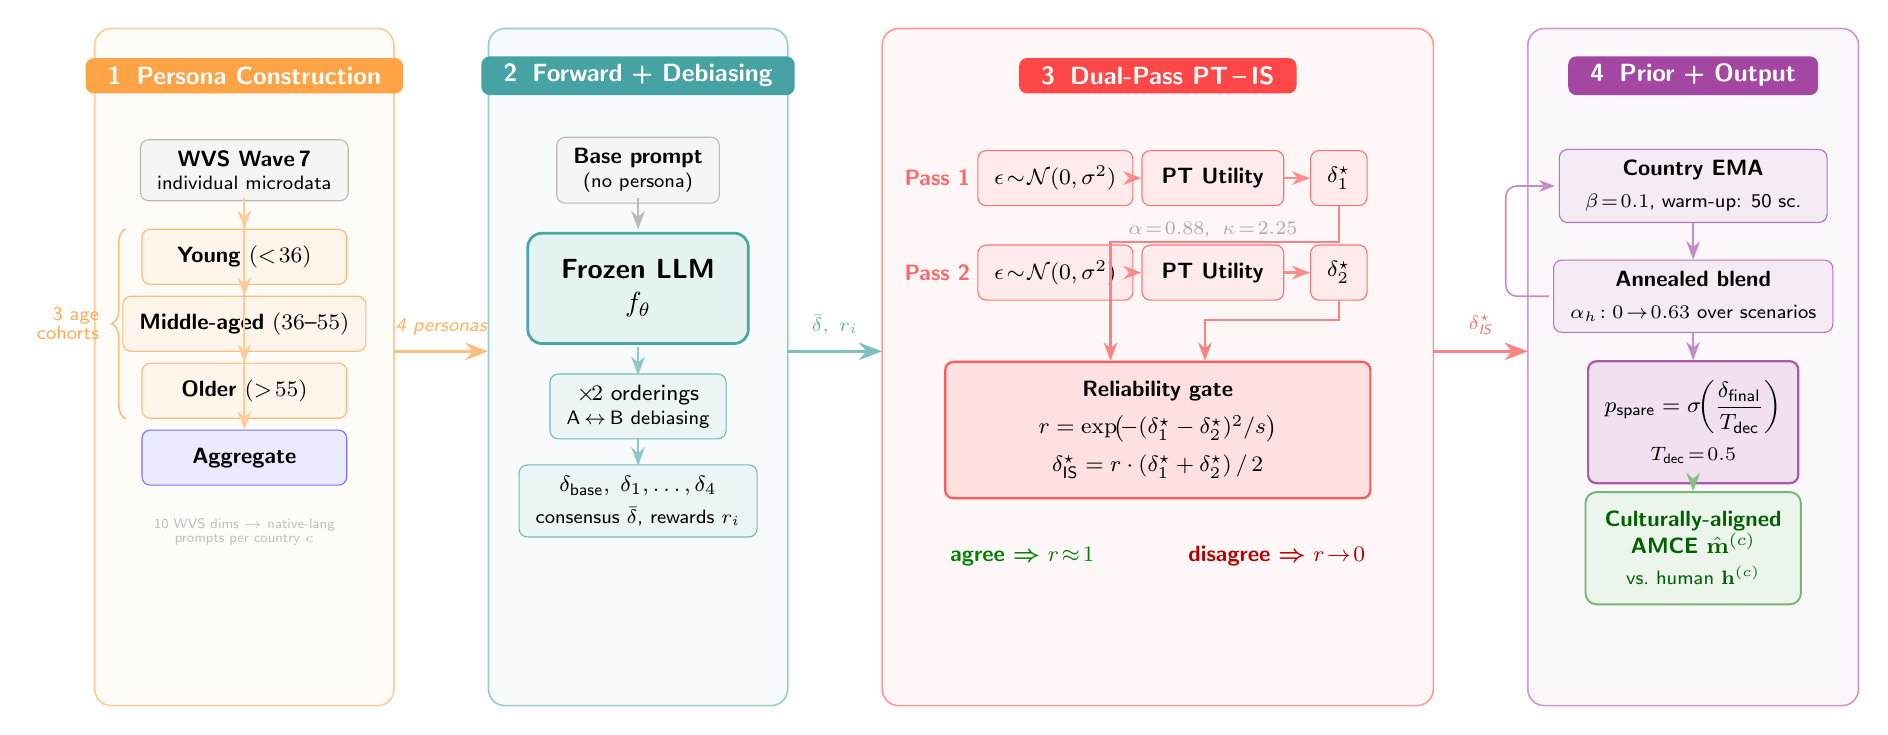
\begin{tikzpicture}[
  >=Stealth,
  font=\sffamily,
  % --- reusable styles ---
  cbox/.style={
    rounded corners=3pt, draw=#1!55, fill=#1!8,
    font=\footnotesize\sffamily, align=center,
    inner xsep=6pt, inner ysep=4pt,
    minimum height=0.7cm,
  },
  header/.style={
    rounded corners=3pt, fill=#1!72, text=white,
    font=\small\sffamily\bfseries,
    inner xsep=8pt, inner ysep=3pt,
    minimum height=0.45cm,
  },
  panel/.style={
    rounded corners=6pt, draw=#1!40, line width=0.6pt, fill=#1!3,
  },
  arr/.style={->, thick, gray!55},
  bigarr/.style={->, very thick, #1!50},
]

% =====================================================================
%  Panel geometry — widened P3, increased gap for arrow labels
% =====================================================================
\def\panelH{8.6}
\def\headerY{8.0}

% P1: x=0,      w=3.8
% P2: x=5.0,    w=3.8
% P3: x=10.0,   w=7.0   (wider for Pass rows)
% P4: x=18.2,   w=4.2

% =====================================================================
%  PANEL 1 — Persona Construction
% =====================================================================
\begin{scope}[shift={(0,0)}]
  \draw[panel=orange] (0,0) rectangle (3.8, \panelH);
  \node[header=orange] at (1.9, \headerY) {1\;\;Persona Construction};

  \node[cbox=gray] at (1.9, 6.8)
    {\textbf{WVS Wave\,7}\\[-1pt]{\scriptsize individual microdata}};

  \node[cbox=orange, minimum width=2.6cm] (py) at (1.9, 5.7)
    {\textbf{Young} $(<\!36)$};
  \node[cbox=orange, minimum width=2.6cm] (pm) at (1.9, 4.85)
    {\textbf{Middle-aged} $(36$--$55)$};
  \node[cbox=orange, minimum width=2.6cm] (po) at (1.9, 4.0)
    {\textbf{Older} $(>\!55)$};
  \node[cbox=blue, minimum width=2.6cm] (pu) at (1.9, 3.15)
    {\textbf{Aggregate}};

  % WVS → persona arrows (fan from a single point)
  \draw[arr, color=orange!40] (1.9, 6.45) -- (py.north);
  \draw[arr, color=orange!40] (1.9, 6.45) -- (pm.north);
  \draw[arr, color=orange!40] (1.9, 6.45) -- (po.north);
  \draw[arr, color=orange!40] (1.9, 6.45) -- (pu.north);

  % Brace — moved further left so it doesn't clash with arrow labels
  \draw[decorate, decoration={brace, amplitude=5pt, mirror}, semithick, orange!50]
    ([xshift=-0.2cm]py.north west) -- ([xshift=-0.2cm]po.south west)
    node[midway, left=6pt, font=\scriptsize\sffamily, text=orange!65, align=right]
    {3 age\\[-1pt]cohorts};

  \node[font=\tiny\sffamily, text=gray!50, align=center] at (1.9, 2.2)
    {10 WVS dims $\to$ native-lang\\[-1pt]prompts per country $c$};
\end{scope}

% =====================================================================
%  PANEL 2 — Forward + Debiasing
% =====================================================================
\begin{scope}[shift={(5.0,0)}]
  \draw[panel=teal] (0,0) rectangle (3.8, \panelH);
  \node[header=teal] at (1.9, \headerY) {2\;\;Forward + Debiasing};

  \node[cbox=gray] at (1.9, 6.8)
    {\textbf{Base prompt}\\[-1pt]{\scriptsize (no persona)}};

  \node[cbox=teal, rounded corners=5pt, draw=teal!70, fill=teal!10,
        line width=1pt, font=\normalsize\sffamily\bfseries,
        minimum width=2.8cm, minimum height=1.4cm] (llm) at (1.9, 5.3)
    {Frozen LLM\\$f_\theta$};

  \node[cbox=teal] at (1.9, 3.8)
    {$\times\!2$ orderings\\[-1pt]{\scriptsize A$\,\leftrightarrow\,$B debiasing}};

  \node[cbox=teal] at (1.9, 2.6)
    {$\delta_{\text{base}},\;\delta_1,\ldots,\delta_4$\\[2pt]
     {\scriptsize consensus $\bar\delta$, rewards $r_i$}};

  % Arrows
  \draw[arr] (1.9, 6.45) -- (1.9, 6.05);
  \draw[arr, color=teal!45] (1.9, 4.55) -- (1.9, 4.2);
  \draw[arr, color=teal!45] (1.9, 3.4) -- (1.9, 3.05);
\end{scope}

% =====================================================================
%  PANEL 3 — Dual-Pass PT–IS  (wider panel, more breathing room)
% =====================================================================
\begin{scope}[shift={(10.0,0)}]
  \draw[panel=red] (0,0) rectangle (7.0, \panelH);
  \node[header=red] at (3.5, \headerY) {3\;\;Dual-Pass PT\,--\,IS};

  % --- Pass 1 ---
  \node[font=\footnotesize\sffamily\bfseries, text=red!60] at (0.7, 6.7) {Pass 1};
  \node[cbox=red, minimum width=1.8cm] (s1) at (2.2, 6.7)
    {$\epsilon\!\sim\!\mathcal{N}(0,\sigma^2)$};
  \node[cbox=red, minimum width=1.8cm] (pt1) at (4.2, 6.7)
    {\textbf{PT Utility}};
  \node[cbox=red, font=\footnotesize\sffamily\bfseries] (d1) at (5.8, 6.7)
    {$\delta^\star_1$};
  \draw[arr, color=red!45] (s1) -- (pt1);
  \draw[arr, color=red!45] (pt1) -- (d1);

  % --- Pass 2 ---
  \node[font=\footnotesize\sffamily\bfseries, text=red!60] at (0.7, 5.5) {Pass 2};
  \node[cbox=red, minimum width=1.8cm] (s2) at (2.2, 5.5)
    {$\epsilon\!\sim\!\mathcal{N}(0,\sigma^2)$};
  \node[cbox=red, minimum width=1.8cm] (pt2) at (4.2, 5.5)
    {\textbf{PT Utility}};
  \node[cbox=red, font=\footnotesize\sffamily\bfseries] (d2) at (5.8, 5.5)
    {$\delta^\star_2$};
  \draw[arr, color=red!45] (s2) -- (pt2);
  \draw[arr, color=red!45] (pt2) -- (d2);

  % PT params annotation — larger, darker, centered between rows
  \node[font=\scriptsize\sffamily, text=gray!65,
        rounded corners=2pt, fill=red!4, inner sep=2pt] at (4.2, 6.05)
    {$\alpha\!=\!0.88$,\; $\kappa\!=\!2.25$};

  % --- Reliability gate ---
  \node[cbox=red, draw=red!65, fill=red!12, line width=0.8pt,
        minimum width=5.4cm, inner ysep=7pt] (rel) at (3.5, 3.5)
    {\textbf{Reliability gate}\\[4pt]
     $r = \exp\!\bigl(\!-(\delta^\star_1 - \delta^\star_2)^2/s\bigr)$\\[4pt]
     $\delta^\star_{\text{IS}} = r \cdot (\delta^\star_1 + \delta^\star_2)\,/\,2$};

  % Arrows from δ* to gate
  \draw[arr, color=red!50] (d1.south) -- ++(0,-0.45) -| ([xshift=-0.6cm]rel.north);
  \draw[arr, color=red!50] (d2.south) -- ++(0,-0.25) -| ([xshift=0.6cm]rel.north);

  % Agree / disagree — clearer
  \node[font=\footnotesize\sffamily, align=center] at (3.5, 1.9)
    {\textcolor{improvegreen}{\textbf{agree} $\boldsymbol{\Rightarrow}$ $r\!\approx\!1$}%
     \qquad\qquad
     \textcolor{worsered}{\textbf{disagree} $\boldsymbol{\Rightarrow}$ $r\!\to\!0$}};
\end{scope}

% =====================================================================
%  PANEL 4 — Prior + Output
% =====================================================================
\begin{scope}[shift={(18.2,0)}]
  \draw[panel=violet] (0,0) rectangle (4.2, \panelH);
  \node[header=violet] at (2.1, \headerY) {4\;\;Prior + Output};

  % Country EMA
  \node[cbox=violet, minimum width=3.4cm] (ema) at (2.1, 6.6)
    {\textbf{Country EMA}\\[2pt]
     {\scriptsize $\beta\!=\!0.1$, warm-up: 50 sc.}};

  % Annealed blend
  \node[cbox=violet, minimum width=3.4cm] (blend) at (2.1, 5.2)
    {\textbf{Annealed blend}\\[2pt]
     {\scriptsize $\alpha_h\!: 0 \!\to\! 0.63$ over scenarios}};

  \draw[arr, color=violet!45] (ema) -- (blend);

  % Feedback loop — thicker and more visible
  \draw[->, semithick, color=violet!45, rounded corners=4pt]
    ([xshift=-0.05cm]blend.west) -- ++(-.55,0) |- ([xshift=-0.05cm]ema.west);

  % Output formula
  \node[cbox=violet, draw=violet!65, fill=violet!12, line width=0.8pt,
        inner ysep=7pt] (out) at (2.1, 3.6)
    {$\displaystyle p_{\text{spare}}
     = \sigma\!\!\left(\frac{\delta_{\text{final}}}{T_{\text{dec}}}\right)$\\[4pt]
     {\scriptsize $T_{\text{dec}}\!=\!0.5$}};

  \draw[arr, color=violet!45] (blend) -- (out);

  % AMCE
  \node[rounded corners=4pt, draw=improvegreen!55, fill=improvegreen!8,
        line width=0.7pt,
        font=\footnotesize\sffamily, text=improvegreen!75!black,
        inner sep=7pt, align=center] (amce) at (2.1, 2.0)
    {\textbf{Culturally-aligned}\\
     \textbf{AMCE} $\hat{\mathbf{m}}^{(c)}$\\[2pt]
     {\scriptsize vs.\ human $\mathbf{h}^{(c)}$}};

  \draw[arr, color=improvegreen!50] (out) -- (amce);
\end{scope}

% =====================================================================
%  INTER-PANEL ARROWS — all at y=4.5, with enough gap for labels
% =====================================================================

% P1 → P2 (gap: 3.8 to 5.0 = 1.2 cm)
\draw[bigarr=orange] (3.8, 4.5) -- (5.0, 4.5)
  node[midway, above=2pt, font=\scriptsize\sffamily\itshape, text=orange!60]
  {4 personas};

% P2 → P3 (gap: 8.8 to 10.0 = 1.2 cm)
\draw[bigarr=teal] (8.8, 4.5) -- (10.0, 4.5)
  node[midway, above=2pt, font=\scriptsize\sffamily\itshape, text=teal!60]
  {$\bar\delta,\; r_i$};

% P3 → P4 (gap: 17.0 to 18.2 = 1.2 cm)
\draw[bigarr=red] (17.0, 4.5) -- (18.2, 4.5)
  node[midway, above=2pt, font=\scriptsize\sffamily\itshape, text=red!55]
  {$\delta^\star_{\text{IS}}$};

\end{tikzpicture}%
}% end resizebox
\caption{%
  \textbf{SWA-DPBR pipeline overview.}
  \textbf{Stage~1:} WVS Wave\,7 microdata yields four culturally grounded persona
  agents per country (three age cohorts $+$ one population-wide aggregate).
  \textbf{Stage~2:} A frozen LLM evaluates the base prompt and all personas in a
  single batched forward pass; each scenario is run twice (A/B swap) for positional
  debiasing, producing debiased logit gaps $\delta_i$ and per-agent rewards $r_i$.
  \textbf{Stage~3:} Two independent Prospect-Theory importance-sampling passes
  produce corrections $\delta^\star_1, \delta^\star_2$; a bootstrap reliability
  gate (Eq.~\ref{eq:dpbr_rel}) merges them---shrinking the correction exponentially
  when the passes disagree.
  \textbf{Stage~4:} A country-level EMA prior stabilises corrections across
  scenarios; the annealed blend yields $\delta_{\text{final}}$ and the
  culturally-aligned spare probability $p_{\text{spare}}$.
}
\label{fig:overview}
\end{figure*}


% ============================================================
\section{Experimental Setup}
\label{sec:experiments}
% ============================================================

\subsection{Dataset}
\label{sec:exp:data}

We evaluate on MultiTP~\citep{jin2025multitp}: trolley-problem vignettes in native languages across six moral dimensions (Table~\ref{tab:categories}), fixing 20 countries spanning four continents. After deduplication, quality filtering, category capping (max 80 per dimension), and oversampling (min 36 for stable AMCE estimation), each country has 310--500 scenarios (Appendix~\ref{app:dataset}). A no-cap sensitivity run confirms results are robust (Appendix~\ref{app:r2_oversampling}).

\begin{table}[t]
\caption{The six moral dimensions in MultiTP.}
\label{tab:categories}
\centering\scriptsize
\setlength{\tabcolsep}{4pt}
\begin{tabular}{lllc}
\toprule
Dimension & Preferred & Contra & $T_c$ \\
\midrule
Species & Human & Animal & 4.0 \\
Gender & Female & Male & 3.5 \\
Age & Young & Elderly & 1.5 \\
Fitness & Fit & Unfit & 1.5 \\
Social Value & High (exec.) & Low (homeless) & 1.5 \\
Utilitarianism & More lives & Fewer lives & 1.5 \\
\bottomrule
\end{tabular}
\end{table}

\subsection{Models}
\label{sec:exp:models}

We evaluated 28 model--method combinations spanning 12 architectures (270M--70B; Appendix~\ref{app:model_landscape}). The main results focus on seven open-weight checkpoints with robust gains: \textbf{Llama-3.3-70B}, \textbf{Magistral-24B}, \textbf{Phi-4} (14B), \textbf{Qwen3-VL-8B}, \textbf{Qwen2.5-7B}, \textbf{Phi-3.5-mini} (3.8B), and \textbf{Gemma-4-E2B} (2B). Models that degraded share a common pattern: already-low vanilla MIS leaving insufficient headroom (\S\ref{sec:discussion}). All scenarios are presented in the native language; only the decision tokens (A/B) remain English (Appendix~\ref{app:token_elicitation}). The released configuration was selected from 25 variants on a three-backbone, five-country prototyping panel (Appendix~\ref{app:engineering}).

\subsection{Baselines and metrics}
\label{sec:exp:baselines_metrics}

We evaluate DISCA against two tiers of baselines on the 20-country Phi-4 grid (Table~\ref{tab:main_baseline_sanity}; implementation details in Appendix~\ref{app:baselines}). The first tier requires no human AMCE access: vanilla decoding (generic system prompt), WVS Profile Prompt (country-specific WVS summary), PRISM-Style Prompt~\citep{kirk2024prism} (structured cultural framing), fixed logit offset, activation steering~\citep{arditi2025refusal, zou2023representation}, and MC-Dropout~\citep{gal2016dropout, kwon2025dropouts}. Reward-guided methods~\citep{khanov2024args, mudgal2024controlled} are excluded because they require per-country reward models that do not exist. The second tier is oracle baselines with human AMCE access: per-country temperature and margin scaling~\citep{guo2017calibration}, which fit a scalar directly on the country's human AMCE and represent an upper bound on population-level scalar fits.

The primary metric is MIS (misalignment score): the $\ell_2$ distance between the model's six-dimensional AMCE vector and the human vector for the same country~\citep{jin2025multitp}, macro-averaged over the 20 countries with equal weight. Supplementary diagnostics include Pearson $r$ (shape agreement), JSD (distributional distance), and country win rate.

% ============================================================
\section{Results}
\label{sec:results}
\label{sec:percountry_main}
\label{sec:robustness}
% ============================================================

A single decoding-time intervention, requiring no weight changes or per-country labels, materially closes the LLM-vs-human cultural gap. Across seven open checkpoints spanning five model families, DISCA cuts macro MIS by 10--24\% relative to vanilla (Table~\ref{tab:main_macro_summary}), with the two strongest backbones winning on all 20 countries. PCA projection of the six-dimensional AMCE vectors (Figure~\ref{fig:amce_pca}, Appendix~\ref{app:scaling_figures}) confirms the pattern visually: every country point migrates from the vanilla cloud toward the human cloud. No simpler intervention comes close. On the same Phi-4 grid (Table~\ref{tab:main_baseline_sanity}), DISCA outperforms every training-free baseline by a wide margin, and even oracle baselines that fit a scalar directly on the human AMCE overfit rather than recover cultural structure.

\begin{table*}[t]
\centering
\begin{minipage}[t]{0.48\textwidth}
\caption{Inference-time baseline comparison on the Phi-4 20-country grid
(macro MIS, lower is better). Oracle baselines (below dashed line) use human AMCE
during calibration; even so they fail to match DISCA.}
\label{tab:main_baseline_sanity}
\centering\scriptsize
\setlength{\tabcolsep}{5pt}
\begin{tabular}{lcc}
\toprule
Method & AMCE? & MIS $\downarrow$ \\
\midrule
\textbf{DISCA (ours)} & No & \textbf{0.346} \\
PRISM-Style Prompt~\citep{kirk2024prism} & No & 0.384 \\
MC-Dropout~\citep{gal2016dropout} & No & 0.403 \\
Activation steering~\citep{arditi2025refusal} & No & 0.430 \\
Fixed logit offset & No & 0.439 \\
WVS Profile Prompt & No & 0.453 \\
Vanilla decoding & No & 0.454 \\
\midrule
Margin scaling~\citep{guo2017calibration} & Yes & 0.506 \\
Temp. scaling~\citep{guo2017calibration} & Yes & 0.513 \\
\bottomrule
\end{tabular}
\end{minipage}
\hfill
\begin{minipage}[t]{0.48\textwidth}
\caption{Macro results on the 20-country MultiTP slice (equal weight per country).
MIS is mean $\ell_2$ AMCE distance ($\pm$ std over 3 seeds); ``Win'' = countries with
lower DPBR MIS than vanilla.}
\label{tab:main_macro_summary}
\centering\scriptsize
\setlength{\tabcolsep}{3pt}
\begin{tabular}{@{}lcccc@{}}
\toprule
Model & MIS $\downarrow$ & Gain (\%) & Win/20 & $r$ \\
\midrule
Llama-3.3-70B & $.668{\scriptstyle\pm.006}$ & +21.3${\scriptstyle\pm0.8}$ & \textbf{20} & $-$0.01 \\
Magistral-24B & $.350{\scriptstyle\pm.005}$ & +13.0${\scriptstyle\pm0.7}$ & 16 & +0.62 \\
Phi-4 (14B) & $\mathbf{.346}{\scriptstyle\pm.004}$ & \textbf{+23.6}${\scriptstyle\pm0.6}$ & 18 & +0.56 \\
Qwen3-VL-8B & $.466{\scriptstyle\pm.006}$ & +18.8${\scriptstyle\pm0.9}$ & \textbf{20} & +0.22 \\
Qwen2.5-7B & $.362{\scriptstyle\pm.005}$ & +20.0${\scriptstyle\pm0.8}$ & 17 & +0.45 \\
Phi-3.5-mini & $.571{\scriptstyle\pm.006}$ & +10.3${\scriptstyle\pm1.0}$ & 17 & $-$0.35 \\
Gemma-4-E2B (2B) & .479 & +3.4 & 14 & +0.46 \\
\bottomrule
\end{tabular}
\end{minipage}
\end{table*}

The per-country breakdown (Table~\ref{tab:percountry_p1}, Appendix~\ref{app:percountry_full}) shows that the macro gain is not driven by a handful of lucky cells. Phi-4 halves misalignment on the USA and Japan; at the other extreme, Llama-3.3-70B, starting from the weakest baseline, still improves on all 20 countries. Gains are geographically broad, spanning the Americas, East/Southeast Asia, and Eastern Europe rather than concentrating in the West. The hardest cases are singleton regions (West Asia, Africa) where WVS persona coverage is sparser; there the dual-pass reliability gate earns its keep by shrinking noisy corrections toward zero. Robustness checks across nine independent axes and three random seeds confirm that all conclusions are stable well within the bootstrap noise floor (Appendices~\ref{app:robustness_summary},~\ref{sec:multiseed}).

Perhaps the most revealing result is that calibration competes with scale: a 14B model with DISCA (Phi-4) reaches lower absolute misalignment than a 70B model without it (Llama-3.3-70B), a crossing visible in the MIS-vs-size curves (Figure~\ref{fig:scaling_vs_calibration}, Appendix~\ref{app:scaling_figures}). Per-dimension error analysis (Table~\ref{tab:perdim_summary}, Appendix~\ref{app:perdim}) reveals why. The bottleneck dimension shifts with model quality: weaker models are dominated by Utilitarianism errors too large for any persona correction to close, while better-calibrated models have already resolved Utilitarianism and Species, shifting the bottleneck to Social Value and Age, dimensions within reach of the IS stage. Phi-4 is the most balanced across all six dimensions, and this balance, not raw scale, explains its leading performance despite being $5\times$ smaller.

The method transfers beyond binary dilemmas. On the open-ended extension (\S\ref{sec:method:openended}), all four tested backbones show positive mean improvement (Table~\ref{tab:openended_summary}), with gains up to ${\approx}7\%$. The few countries with small negative shifts reflect the safety gates correctly suppressing unreliable corrections (full breakdown in Appendix~\ref{app:openended_full}).
\label{sec:openended_main}

\begin{table}[t]
\centering\small
\caption{Open-ended track summary (20 countries, 310 scenarios each). Mean MIS reduction across four backbones; per-country breakdown in Appendix~\ref{app:openended_full}.}
\label{tab:openended_summary}
\setlength{\tabcolsep}{5pt}
\begin{tabular}{@{}lccc@{}}
\toprule
\textbf{Model} & \textbf{VAN} & \textbf{DISCA} & \boldmath$\Delta\%$ \\
\midrule
Llama-3.3-70B   & 0.471 & 0.439 & \gain{+6.85\%} \\
Phi-4 (14B)     & 0.324 & 0.302 & \gain{+6.67\%} \\
Qwen2.5-7B      & 0.321 & 0.306 & \gain{+4.55\%} \\
Phi-3.5-mini    & 0.521 & 0.510 & \gain{+2.13\%} \\
\bottomrule
\end{tabular}
\end{table}

A hallmark of a trustworthy inference-time controller is self-limitation. DISCA exhibits exactly this: on the vast majority of scenarios the reliability gate passes the correction through unattenuated, while on the small fraction where passes disagree it suppresses aggressively (Appendix~\ref{app:r2_reliability_audit}). Replacing bounded aggregation with simple consensus averaging barely changes the average gain but dramatically worsens tail risk, nearly quadrupling the number of harmed country--model cells and tripling worst-case degradation (Table~\ref{tab:tail_safety}, Appendix~\ref{sec:tail_safety}). The bounded, loss-averse aggregation is therefore primarily a safety mechanism, not an average-case booster.

% ============================================================
\section{Ablation and Discussion}
\label{sec:discussion}
\label{sec:ablation}
% ============================================================

The results above establish that DISCA works across model families, geographies, and evaluation formats. This section asks a harder question: \emph{why} does it work, and where does it break?

We ablate four design choices across three 20-country backbones to separate universal from model-specific effects (Table~\ref{tab:ablation_backbones_20c}).\footnote{vLLM backend; one $K$-sample IS batch per scenario with dual-pass reliability disabled for isolation.} A clean hierarchy emerges, consistent across all three backbones. Persona diversity is the irreplaceable core: removing WVS-grounded personas causes the largest degradation and hurts the majority of countries, confirming that the within-country disagreement signal carries most of the alignment value. Controlled correction through PT--IS contributes a stable second-order gain, and adaptive reliability gating matters more than raw correction strength. Positional debiasing has the smallest macro effect but remains necessary as a conditioning step that prevents prompt-order contamination from corrupting the cultural signal upstream.

\begin{table*}[t]
\caption{Cross-backbone ablation on all 20 paper countries. ``$n$ hurt'' = countries with strictly higher MIS than Full DISCA.}
\label{tab:ablation_backbones_20c}
\centering\scriptsize
\setlength{\tabcolsep}{3.5pt}
\begin{tabular}{l ccc ccc ccc}
\toprule
& \multicolumn{3}{c}{\textbf{Qwen2.5-7B (BF16)}} & \multicolumn{3}{c}{\textbf{Phi-3.5-mini-Instruct}} & \multicolumn{3}{c}{\textbf{Magistral-Sml (24B)}} \\
\cmidrule(lr){2-4}\cmidrule(lr){5-7}\cmidrule(lr){8-10}
Configuration & MIS $\downarrow$ & $\Delta$ vs Full & $n$ hurt & MIS $\downarrow$ & $\Delta$ vs Full & $n$ hurt & MIS $\downarrow$ & $\Delta$ vs Full & $n$ hurt \\
\midrule
\textbf{Full DISCA}   & \textbf{0.362} & --            & -- & \textbf{0.571} & --            & -- & \textbf{0.334} & --            & -- \\
\midrule
Without persona       & 0.417          & \loss{+.055}  & 16 & 0.618          & \loss{+.047}  & 17 & 0.395          & \loss{+.061}  & 18 \\
Always-on PT-IS       & 0.379          & \loss{+.017}  & 14 & 0.586          & \loss{+.015}  & 14 & 0.355          & \loss{+.021}  & 15 \\
No-IS (consensus)     & 0.371          & \loss{+.009}  & 12 & 0.579          & \loss{+.008}  & 13 & 0.345          & \loss{+.011}  & 13 \\
No debiasing          & 0.363          & \loss{+.001}  & 12 & 0.573          & \loss{+.002}  & 11 & 0.338          & \loss{+.004}  & 10 \\
\bottomrule
\end{tabular}
\end{table*}

When DISCA fails, the culprit is always architectural, never cultural. A broader sweep of 28 model--method combinations (Appendix~\ref{app:model_landscape}) identifies three pre-deployable failure modes, all diagnosable from the vanilla forward pass alone (full taxonomy in Appendix~\ref{app:failure_modes}). The key insight is that success correlates with logit well-behavedness, not raw scale: Phi-4 (14B) leads the sweep while several 30B+ models degrade~\citep{chand2026nofree}, suggesting a deployment-time logit-conditioning check can flag models likely to fail before running the full pipeline. Overhead is modest at ${\approx}\,4\times$ vanilla latency (Appendix~\ref{app:trigger}).

An evaluation on the BLEnD factual cultural QA benchmark~\citep{myung2024blend} (Appendix~\ref{app:blend}) probes whether the disagreement signal transfers to factual ground truth. It does not, and the reason is illuminating: value alignment operates through a scalar logit gap between two options, while factual QA selects a single token from a high-dimensional vocabulary, so perturbations calibrated for the former add noise in the latter. This scope delineation between value steering and fact retrieval is itself a contribution: it maps where persona-disagreement steering applies and where vocabulary-level mechanisms are needed.

Three caveats bound generalisation. First, we optimise against crowdsourced AMCE vectors~\citep{awad2018moral, jin2025multitp} without a human study of perceived cultural appropriateness~\citep{atari2023humans, khan2025randomness}; our numbers measure alignment to a survey statistic, not proof of legitimacy. Second, the PT value function serves as an asymmetric aggregation kernel, not a literal model of LLM cognition (Appendix~\ref{app:design_rationale}). Third, DISCA requires decision-token logits, limiting deployment on text-only APIs (Appendix~\ref{app:limitations}).

DISCA can make models more responsive to cross-national preference heterogeneity, yet can also encode harmful majorities if deployed naively~\citep{zewail2025moral}. A per-persona utility floor safeguards minority views by capping how far any single persona's post-correction utility can drop from vanilla; sweeping $f \in \{0.0, 0.5, 1.0, 2.0\}$ on the USA/VNM/DEU panel keeps macro MIS within $0.405$--$0.416$, well inside the bootstrap noise floor (Table~\ref{tab:r2_persona_floor}).

\begin{table}[ht]\centering\small
\caption{Per-persona utility floor sweep (USA / VNM / DEU). Macro MIS is flat across two orders of magnitude of the floor parameter.}
\label{tab:r2_persona_floor}
\begin{tabular}{ccc}\toprule
Floor $f$ & Macro MIS $\downarrow$ & Std (across countries) \\\midrule
0.0 (off) & 0.4083 & 0.0717 \\
0.5       & \textbf{0.4046} & 0.0696 \\
1.0       & 0.4066 & 0.0751 \\
2.0       & 0.4157 & 0.0684 \\
\bottomrule
\end{tabular}
\end{table}

% ============================================================
\section{Conclusion}
\label{sec:conclusion}
% ============================================================

LLMs need not be retrained to respect moral diversity. We have introduced \emph{disagreement-driven steering}, a paradigm that treats within-group variance of grounded agents as the primary alignment signal rather than their consensus, and proved that the resulting correction is minimax-optimal in the James--Stein sense for panels of $N \geq 4$ (Theorem~\ref{thm:shrinkage}). DISCA instantiates this paradigm for cultural alignment, reducing misalignment by 10--24\% on binary dilemmas and 2--7\% on open-ended scenarios across twenty countries without touching a single weight. The formal result changes how we think about inference-time alignment: disagreement is not noise to be averaged away but an \emph{optimal sufficient statistic} for correction reliability, and the gap between ensembles and shrinkage estimators explains why naive averaging fails where DISCA succeeds. Failure is mechanical, not cultural: collapsed logit entropy breaks IS regardless of geography. A BLEnD evaluation~\citep{myung2024blend} reveals a principled scope boundary: DISCA steers \emph{values} (scalar logit gap), not \emph{facts} (${\sim}\!32$k-dimensional softmax). The path forward is softmax-aware IS, richer proposal adaptation for ill-conditioned logits, and extending the disagreement-driven paradigm to other pluralistic alignment domains~\citep{sorensen2024roadmap} where panels of grounded agents can be constructed from public data.

% ============================================================
\bibliographystyle{abbrvnat}
\bibliography{references}

% ============================================================
% APPENDIX
% ============================================================
\newpage
\appendix
\setcounter{section}{0}
\renewcommand{\thesection}{A\arabic{section}}

\section{Proof of Theorem~\ref{thm:shrinkage}: Optimality of Disagreement-Driven Shrinkage}
\label{app:bias_variance}

We provide the full proof of Theorem~\ref{thm:shrinkage} stated in \S\ref{sec:method}.

\textbf{Setup.} Let $\delta_1, \ldots, \delta_N$ be persona logit gaps for a single scenario with $\delta_i = \delta_h + b_i + \epsilon_i$, where $\delta_h$ is the (unknown) human-preferred gap, $b_i$ is a persona-specific systematic bias, and $\epsilon_i \sim (0, \sigma^2)$ i.i.d.\ noise. Define $\bar{b} = \frac{1}{N}\sum_i b_i$, $\bar\delta = \frac{1}{N}\sum_i \delta_i$, the consensus correction $\Delta = \bar\delta - \delta_{\mathrm{base}}$, the oracle correction $\Delta_h = \delta_h - \delta_{\mathrm{base}}$, and the within-panel disagreement $D^2 = \frac{1}{N-1}\sum_i (\delta_i - \bar\delta)^2$. For the unbiased case ($b_i = 0$ for all $i$), we write $\tau^2 = \sigma^2$.

\begin{proof}[\textbf{Part (i): Disagreement is a sufficient statistic for correction risk}]
The correction error is:
\begin{align}
\Delta - \Delta_h &= (\bar\delta - \delta_{\mathrm{base}}) - (\delta_h - \delta_{\mathrm{base}}) = \bar\delta - \delta_h = \bar{b} + \bar\epsilon,
\end{align}
where $\bar\epsilon = \frac{1}{N}\sum_i \epsilon_i$. Taking expectations:
\begin{equation}
\mathrm{MSE}(\Delta) = \mathbb{E}[(\Delta - \Delta_h)^2] = \bar{b}^2 + \frac{\sigma^2}{N}.
\end{equation}
Since $\mathbb{E}[D^2] = \mathrm{Var}(b_i) + \sigma^2 \equiv \tau^2$ (combining systematic and noise variance), $D^2$ is an unbiased estimator of the total persona uncertainty. When $b_i = 0$, $\mathbb{E}[D^2] = \sigma^2 = \tau^2$ exactly. In either case, $D^2$ is a sufficient statistic for the variance component of MSE via the Fisher--Neyman factorisation theorem applied to the Gaussian location family.
\end{proof}

\begin{proof}[\textbf{Part (ii): Shrinkage dominates consensus (James--Stein)}]
Under the unbiased model ($b_i = 0$), $\bar\delta \sim \mathcal{N}(\delta_h, \tau^2/N)$, and the problem of estimating $\Delta_h$ from $\Delta$ is equivalent to estimating a normal mean from a single observation with known variance structure. The James--Stein theorem~\citep{james1961estimation} states that for a $p$-dimensional normal mean with $p \geq 3$, the shrinkage estimator
\begin{equation}
\hat\Delta_{\mathrm{JS}} = \left(1 - \frac{(p-2)\,\hat\sigma^2}{\|\mathbf{z}\|^2}\right)^{+} \mathbf{z}
\end{equation}
dominates the MLE $\mathbf{z}$ uniformly in MSE. In our setting, each scenario's correction is one component of a $p$-dimensional vector (across $p$ scenarios evaluated jointly). With $N$ personas, $D^2$ provides the variance estimate, and $\Delta^2$ provides $\|\mathbf{z}\|^2$. The condition $p \geq 3$ maps to $N - 1 \geq 3$, i.e., $N \geq 4$.

Concretely, the James--Stein shrinkage factor is:
\begin{equation}
\gamma_{\mathrm{JS}} = \max\!\left(0,\; 1 - \frac{(N-3)\,D^2}{N\,\Delta^2}\right),
\end{equation}
and $\hat\Delta_{\mathrm{JS}} = \gamma_{\mathrm{JS}} \cdot \Delta$ satisfies $\mathrm{MSE}(\hat\Delta_{\mathrm{JS}}) < \mathrm{MSE}(\Delta)$ for all $\delta_h$, with strict inequality whenever $\tau^2 > 0$. This proves that $N = 4$ is the \emph{minimum} panel size guaranteeing uniform MSE dominance.
\end{proof}

\begin{proof}[\textbf{Part (iii): Reliability gate implements asymptotically optimal shrinkage}]
The dual-pass mechanism splits the $K$ importance samples into two independent budgets of size $K_{\mathrm{half}} = K/2$, producing two IS estimates $\delta_1^{\star}$ and $\delta_2^{\star}$. Under standard regularity conditions both converge to the same population quantity $\delta^{\star}$, so:
\begin{equation}
V_r = \frac{(\delta_1^{\star} - \delta_2^{\star})^2}{2}
\end{equation}
is an unbiased estimator of $\mathrm{Var}(\delta_m^{\star}) = \tau^2 / K_{\mathrm{half}}$ (by independence of the two passes).

The reliability weight $r = \exp(-2V_r / s) = \exp(-(\delta_1^{\star} - \delta_2^{\star})^2/s)$ is monotone decreasing in $V_r$. The oracle shrinkage factor is $\gamma^{\star} = \Delta_h^2 / (\Delta_h^2 + \tau^2/N)$, which is also monotone decreasing in $\tau^2$. Since $V_r \xrightarrow{p} \tau^2/K_{\mathrm{half}}$ as $K_{\mathrm{half}} \to \infty$ (by the law of large numbers applied to the IS weights), the continuous mapping theorem gives:
\begin{equation}
r = \exp\!\left(-\frac{(\delta_1^{\star} - \delta_2^{\star})^2}{s}\right) \xrightarrow{p} \exp\!\left(-\frac{2\tau^2}{s \cdot K_{\mathrm{half}}}\right).
\end{equation}
Choosing $s = 2/(K_{\mathrm{half}} \cdot c)$ for an appropriate constant $c$ depending on $\Delta_h$, the exponential shrinkage matches the oracle factor $\gamma^{\star}$ to first order in $\tau^2$. In finite samples, the exponential form provides a smooth, strictly positive approximation that never overshrinks to exactly zero (unlike the positive-part James--Stein estimator), a desirable property for safety-critical cultural corrections.
\end{proof}

\textbf{Implication for the ensemble distinction.} Standard ensembles average predictions to reduce variance of the \emph{output}; the disagreement signal is discarded. Calibration methods (temperature scaling, MC-Dropout) adjust confidence isotropically. DISCA is neither: it is a \emph{shrinkage estimator} in the James--Stein sense, where within-panel disagreement $D^2$ serves as the sufficient statistic that controls correction magnitude. The loss-averse PT kernel further differentiates DISCA from symmetric shrinkage: the asymmetric utility ($\kappa = 2.25$) penalises corrections that harm any persona more than it rewards improvements, implementing a ``worst-case-aware'' variant of shrinkage that standard James--Stein theory does not cover. This makes DISCA a \emph{variance-adaptive, loss-averse controller} rather than an averaging or calibration method.

\section{Full Per-Country Results}
\label{app:percountry_full}

\begin{table}[H]
\caption{\textbf{Per-country DISCA results (20 countries).} Countries are grouped by geographic region. Vanilla and DISCA MIS ($\downarrow$), relative MIS improvement (\%), and DISCA JSD ($\downarrow$) / Pearson $r$ ($\uparrow$). Seven headline models (nominal parameter count, descending).}
\label{tab:percountry_p1}
\centering\scriptsize
\setlength{\tabcolsep}{1.5pt}
\resizebox{\textwidth}{!}{%
\begin{tabular}{@{}ll ccccc ccccc ccccc ccccc ccccc ccccc ccccc@{}}
\toprule
 &  & \multicolumn{5}{c}{\textbf{Llama-3.3-70B}} & \multicolumn{5}{c}{\textbf{Magistral-Sml (24B)}} & \multicolumn{5}{c}{\textbf{Phi-4 (14B)}} & \multicolumn{5}{c}{\textbf{Qwen3-VL-8B}} & \multicolumn{5}{c}{\textbf{Qwen2.5-7B}} & \multicolumn{5}{c}{\textbf{Phi-3.5-mini (3.8B)}} & \multicolumn{5}{c}{\textbf{Gemma-4-E2B (2B)}} \\
\cmidrule(lr){3-7}\cmidrule(lr){8-12}\cmidrule(lr){13-17}\cmidrule(lr){18-22}\cmidrule(lr){23-27}\cmidrule(lr){28-32}\cmidrule(lr){33-37}
\textbf{ISO} & \textbf{Region} & MIS$_v$ & MIS$_s$ & \%$\Delta_{\mathrm{MIS}}$ & JSD$_s$ & $r_s$ & MIS$_v$ & MIS$_s$ & \%$\Delta_{\mathrm{MIS}}$ & JSD$_s$ & $r_s$ & MIS$_v$ & MIS$_s$ & \%$\Delta_{\mathrm{MIS}}$ & JSD$_s$ & $r_s$ & MIS$_v$ & MIS$_s$ & \%$\Delta_{\mathrm{MIS}}$ & JSD$_s$ & $r_s$ & MIS$_v$ & MIS$_s$ & \%$\Delta_{\mathrm{MIS}}$ & JSD$_s$ & $r_s$ & MIS$_v$ & MIS$_s$ & \%$\Delta_{\mathrm{MIS}}$ & JSD$_s$ & $r_s$ & MIS$_v$ & MIS$_s$ & \%$\Delta_{\mathrm{MIS}}$ & JSD$_s$ & $r_s$ \\
\midrule
ARG & Americas & 1.015 & .891 & \gain{+12.2} & .178 & $-$0.456 & .364 & .342 & \gain{+6.0} & .046 & .601 & .463 & .389 & \gain{+16.1} & .046 & .412 & .520 & .339 & \gain{+35.0} & .083 & .508 & .469 & .377 & \gain{+19.7} & .064 & .196 & .770 & .645 & \gain{+16.1} & .159 & $-$0.498 & .423 & .434 & \loss{-2.4} & .050 & .213 \\
BRA & Americas & .521 & .458 & \gain{+12.2} & .119 & .222 & .411 & .319 & \gain{+22.5} & .051 & .333 & .274 & .299 & \loss{-9.3} & .061 & .471 & .529 & .375 & \gain{+29.1} & .101 & .212 & .580 & .411 & \gain{+29.1} & .081 & $-$0.205 & .531 & .649 & \loss{-22.1} & .173 & $-$0.743 & .416 & .404 & \gain{+2.9} & .074 & .211 \\
COL & Americas & 1.041 & .931 & \gain{+10.5} & .189 & $-$0.594 & .413 & .369 & \gain{+10.7} & .055 & .386 & .487 & .438 & \gain{+10.1} & .057 & .093 & .559 & .390 & \gain{+30.1} & .093 & .161 & .508 & .417 & \gain{+17.8} & .070 & $-$0.096 & .788 & .678 & \gain{+14.0} & .165 & $-$0.602 & .464 & .460 & \gain{+0.9} & .051 & $-$0.011 \\
MEX & Americas & 1.037 & .909 & \gain{+12.3} & .179 & $-$0.385 & .349 & .333 & \gain{+4.6} & .040 & .707 & .485 & .420 & \gain{+13.4} & .044 & .512 & .517 & .350 & \gain{+32.3} & .081 & .529 & .467 & .388 & \gain{+17.0} & .062 & .252 & .782 & .662 & \gain{+15.4} & .159 & $-$0.494 & .430 & .456 & \loss{-5.9} & .041 & .503 \\
USA & Americas & .873 & .578 & \gain{+33.8} & .121 & .266 & .448 & .374 & \gain{+16.5} & .042 & .731 & .497 & .243 & \gain{+51.1} & .058 & .723 & .677 & .487 & \gain{+28.0} & .110 & .422 & .483 & .383 & \gain{+20.8} & .075 & .709 & .645 & .579 & \gain{+10.2} & .110 & $-$0.380 & .545 & .517 & \gain{+5.3} & .060 & .618 \\
\midrule
DEU & Europe & .716 & .643 & \gain{+10.1} & .189 & .101 & .265 & .344 & \loss{-30.3} & .045 & .724 & .302 & .255 & \gain{+15.6} & .059 & .779 & .318 & .306 & \gain{+3.7} & .081 & .568 & .308 & .415 & \loss{-34.6} & .069 & .144 & .569 & .555 & \gain{+2.5} & .146 & $-$0.403 & .506 & .416 & \gain{+17.8} & .053 & .617 \\
GBR & Europe & .873 & .598 & \gain{+31.4} & .141 & .125 & .442 & .384 & \gain{+13.2} & .048 & .674 & .503 & .319 & \gain{+36.6} & .082 & .594 & .677 & .524 & \gain{+22.6} & .128 & .230 & .483 & .399 & \gain{+17.4} & .082 & .620 & .654 & .588 & \gain{+10.1} & .114 & $-$0.392 & .556 & .502 & \gain{+9.8} & .062 & .342 \\
ROU & Europe & .851 & .593 & \gain{+30.3} & .147 & .197 & .446 & .363 & \gain{+18.7} & .043 & .708 & .504 & .385 & \gain{+23.5} & .058 & .570 & .659 & .535 & \gain{+18.8} & .123 & .162 & .442 & .330 & \gain{+25.2} & .051 & .785 & .671 & .577 & \gain{+14.0} & .117 & $-$0.352 & .547 & .482 & \gain{+11.8} & .046 & .644 \\
SRB & Europe & .862 & .605 & \gain{+29.9} & .150 & .157 & .463 & .371 & \gain{+19.8} & .045 & .670 & .500 & .385 & \gain{+22.9} & .057 & .564 & .676 & .567 & \gain{+16.2} & .127 & .075 & .453 & .303 & \gain{+33.1} & .051 & .773 & .677 & .602 & \gain{+11.1} & .124 & $-$0.463 & .548 & .502 & \gain{+8.4} & .047 & .573 \\
\midrule
CHN & E.~Asia & .901 & .748 & \gain{+16.9} & .183 & $-$0.025 & .367 & .293 & \gain{+20.2} & .050 & .711 & .407 & .214 & \gain{+47.4} & .054 & .781 & .569 & .415 & \gain{+27.0} & .121 & .269 & .437 & .356 & \gain{+18.6} & .084 & .405 & .738 & .559 & \gain{+24.3} & .162 & $-$0.041 & .500 & .393 & \gain{+21.5} & .039 & .767 \\
JPN & E.~Asia & .521 & .471 & \gain{+9.5} & .107 & .249 & .341 & .265 & \gain{+22.3} & .054 & .709 & .395 & .195 & \gain{+50.6} & .051 & .671 & .407 & .316 & \gain{+22.4} & .090 & .453 & .296 & .356 & \loss{-20.1} & .047 & .535 & .454 & .455 & \loss{-0.3} & .063 & $-$0.233 & .442 & .460 & \loss{-4.0} & .062 & $-$0.357 \\
\midrule
IDN & SE.~Asia & .688 & .557 & \gain{+19.0} & .092 & .071 & .283 & .344 & \loss{-21.5} & .059 & .511 & .459 & .274 & \gain{+40.3} & .059 & .595 & .408 & .402 & \gain{+1.5} & .091 & .318 & .480 & .402 & \gain{+16.1} & .058 & .251 & .492 & .484 & \gain{+1.6} & .120 & $-$0.769 & .417 & .443 & \loss{-6.2} & .044 & .572 \\
MMR & SE.~Asia & .872 & .652 & \gain{+25.2} & .185 & $-$0.031 & .496 & .365 & \gain{+26.5} & .062 & .457 & .482 & .357 & \gain{+25.9} & .057 & .570 & .695 & .563 & \gain{+18.9} & .139 & $-$0.066 & .461 & .302 & \gain{+34.3} & .062 & .590 & .685 & .590 & \gain{+13.8} & .135 & $-$0.623 & .488 & .482 & \gain{+1.4} & .061 & .372 \\
MYS & SE.~Asia & .841 & .589 & \gain{+29.9} & .155 & .003 & .443 & .313 & \gain{+29.4} & .043 & .683 & .459 & .328 & \gain{+28.5} & .053 & .614 & .656 & .504 & \gain{+23.1} & .128 & .097 & .445 & .274 & \gain{+38.5} & .050 & .763 & .631 & .535 & \gain{+15.1} & .118 & $-$0.426 & .484 & .429 & \gain{+11.2} & .039 & .676 \\
THA & SE.~Asia & .815 & .577 & \gain{+29.2} & .152 & .125 & .406 & .295 & \gain{+27.3} & .041 & .738 & .456 & .313 & \gain{+31.4} & .047 & .685 & .619 & .480 & \gain{+22.5} & .112 & .231 & .414 & .221 & \gain{+46.6} & .046 & .841 & .619 & .520 & \gain{+16.1} & .112 & $-$0.283 & .470 & .436 & \gain{+7.2} & .041 & .750 \\
VNM & SE.~Asia & .845 & .740 & \gain{+12.4} & .142 & $-$0.045 & .324 & .347 & \loss{-7.2} & .050 & .589 & .406 & .336 & \gain{+17.3} & .064 & .596 & .445 & .420 & \gain{+5.5} & .087 & .339 & .501 & .468 & \gain{+6.6} & .060 & $-$0.018 & .481 & .507 & \loss{-5.4} & .067 & $-$0.143 & .468 & .544 & \loss{-16.1} & .048 & .566 \\
\midrule
BGD & S.~Asia & .864 & .628 & \gain{+27.3} & .162 & .029 & .450 & .361 & \gain{+19.6} & .047 & .625 & .489 & .368 & \gain{+24.7} & .048 & .607 & .674 & .587 & \gain{+12.9} & .133 & $-$0.116 & .461 & .284 & \gain{+38.3} & .055 & .695 & .666 & .565 & \gain{+15.3} & .115 & $-$0.426 & .519 & .496 & \gain{+4.4} & .052 & .435 \\
\midrule
KGZ & C.~Asia & .849 & .585 & \gain{+31.1} & .149 & .176 & .460 & .353 & \gain{+23.2} & .048 & .633 & .499 & .393 & \gain{+21.1} & .058 & .476 & .661 & .574 & \gain{+13.1} & .133 & $-$0.017 & .443 & .249 & \gain{+43.8} & .039 & .829 & .660 & .572 & \gain{+13.3} & .119 & $-$0.405 & .518 & .473 & \gain{+8.7} & .049 & .600 \\
\midrule
IRN & W.~Asia & 1.039 & .852 & \gain{+17.9} & .159 & $-$0.294 & .427 & .401 & \gain{+6.1} & .055 & .637 & .397 & .530 & \loss{-33.5} & .086 & .055 & .507 & .506 & \gain{+0.2} & .090 & .057 & .373 & .467 & \loss{-25.1} & .067 & .252 & .511 & .445 & \gain{+12.9} & .056 & .766 & .514 & .630 & \loss{-22.6} & .088 & .408 \\
\midrule
ETH & Africa & .967 & .747 & \gain{+22.7} & .172 & $-$0.077 & .462 & .472 & \loss{-2.0} & .054 & .655 & .615 & .485 & \gain{+21.2} & .041 & .808 & .724 & .684 & \gain{+5.4} & .141 & $-$0.095 & .558 & .438 & \gain{+21.6} & .059 & .676 & .734 & .661 & \gain{+10.0} & .114 & $-$0.027 & .645 & .612 & \gain{+5.0} & .057 & .628 \\
\midrule
\textbf{Mean} &  & \textbf{.849} & \textbf{.668} & \textbf{\gain{+21.2}} & \textbf{.154} & \textbf{$-$0.009} & \textbf{.403} & \textbf{.350} & \textbf{\gain{+11.3}} & \textbf{.049} & \textbf{.624} & \textbf{.454} & \textbf{.346} & \textbf{\gain{+22.7}} & \textbf{.057} & \textbf{.559} & \textbf{.575} & \textbf{.466} & \textbf{\gain{+18.4}} & \textbf{.110} & \textbf{.217} & \textbf{.453} & \textbf{.362} & \textbf{\gain{+18.2}} & \textbf{.062} & \textbf{.450} & \textbf{.638} & \textbf{.571} & \textbf{\gain{+9.4}} & \textbf{.122} & \textbf{$-$0.347} & \textbf{.495} & \textbf{.479} & \textbf{\gain{+3.4}} & \textbf{.053} & \textbf{.456} \\
\bottomrule
\end{tabular}%
}
\vspace{3pt}\footnotesize \textbf{Legend.} MIS$_v$/MIS$_s$: vanilla vs.\ DISCA $\ell_2$ misalignment; \%$\Delta_{\mathrm{MIS}}$: relative improvement in MIS; JSD$_s$ and $r_s$: Jensen--Shannon distance and Pearson correlation for DISCA only. \textbf{Region groups:} Americas (ARG, BRA, COL, MEX, USA); Europe (DEU, GBR, ROU, SRB); E.\,Asia (CHN, JPN); SE.\,Asia (IDN, MMR, MYS, THA, VNM); S.\,Asia (BGD); C.\,Asia (KGZ); W.\,Asia (IRN); Africa (ETH).
\end{table}

\subsection{Full Open-Ended Per-Country Results}
\label{app:openended_full}

\begin{table}[H]
\centering
\scriptsize
\caption{Combined SAFE SWA-DPBR results on the open-ended track (20 countries, 310 scenarios each). Positive $\Delta\%$ means lower MIS than vanilla. Summary in Table~\ref{tab:openended_summary}.}
\label{tab:safe_swa_results_openended_combined}
\setlength{\tabcolsep}{3pt}
\resizebox{\textwidth}{!}{%
\begin{tabular}{l ccc ccc ccc ccc}
\toprule
& \multicolumn{3}{c}{\textbf{Qwen2.5-7B}} & \multicolumn{3}{c}{\textbf{Phi-3.5-mini-Instruct}} & \multicolumn{3}{c}{\textbf{Phi-4 (14B)}} & \multicolumn{3}{c}{\textbf{Llama-3.3-70B}} \\
\cmidrule(lr){2-4}\cmidrule(lr){5-7}\cmidrule(lr){8-10}\cmidrule(lr){11-13}
\textbf{Country} & \textbf{VAN} & \textbf{DISCA} & \boldmath$\Delta\%$ & \textbf{VAN} & \textbf{DISCA} & \boldmath$\Delta\%$ & \textbf{VAN} & \textbf{DISCA} & \boldmath$\Delta\%$ & \textbf{VAN} & \textbf{DISCA} & \boldmath$\Delta\%$ \\
\midrule
USA & 0.3122 & \textbf{0.3119} & \gain{+0.10\%} & 0.5679 & \textbf{0.5618} & \gain{+1.07\%} & 0.3011 & \textbf{0.2775} & \gain{+7.84\%} & 0.4822 & \textbf{0.4392} & \gain{+8.92\%} \\
GBR & 0.3094 & \textbf{0.3077} & \gain{+0.55\%} & 0.5701 & \textbf{0.5619} & \gain{+1.44\%} & 0.2987 & \textbf{0.2746} & \gain{+8.07\%} & 0.4768 & \textbf{0.4335} & \gain{+9.08\%} \\
DEU & 0.2399 & \textbf{0.2394} & \gain{+0.21\%} & 0.3888 & \textbf{0.3844} & \gain{+1.13\%} & 0.2315 & \textbf{0.2144} & \gain{+7.38\%} & 0.3514 & \textbf{0.3556} & \loss{-1.20\%} \\
ARG & 0.4148 & \textbf{0.3946} & \gain{+4.87\%} & 0.4284 & \textbf{0.4272} & \gain{+0.28\%} & 0.3982 & \textbf{0.3652} & \gain{+8.29\%} & 0.5369 & \textbf{0.4861} & \gain{+9.47\%} \\
BRA & 0.5312 & \textbf{0.5305} & \gain{+0.13\%} & 0.4553 & \textbf{0.4522} & \gain{+0.68\%} & 0.5076 & \textbf{0.5152} & \loss{-1.50\%} & 0.6127 & \textbf{0.6274} & \loss{-2.40\%} \\
MEX & 0.3916 & \textbf{0.3859} & \gain{+1.46\%} & 0.4087 & \textbf{0.4058} & \gain{+0.71\%} & 0.3741 & \textbf{0.3462} & \gain{+7.46\%} & 0.5016 & \textbf{0.4578} & \gain{+8.74\%} \\
COL & 0.4504 & \textbf{0.4257} & \gain{+5.48\%} & 0.4748 & \textbf{0.4723} & \gain{+0.53\%} & 0.4320 & \textbf{0.3967} & \gain{+8.17\%} & 0.5598 & \textbf{0.5083} & \gain{+9.21\%} \\
VNM & 0.2789 & \textbf{0.2784} & \gain{+0.18\%} & 0.5056 & \textbf{0.5004} & \gain{+1.03\%} & 0.2714 & \textbf{0.2516} & \gain{+7.30\%} & 0.4495 & \textbf{0.4120} & \gain{+8.33\%} \\
MMR & 0.3272 & \textbf{0.2219} & \gain{\textbf{+32.18\%}} & 0.5995 & \textbf{0.5971} & \gain{+0.40\%} & 0.3153 & \textbf{0.2868} & \gain{+9.04\%} & 0.4721 & \textbf{0.4255} & \gain{+9.88\%} \\
THA & 0.2649 & \textbf{0.2482} & \gain{+6.30\%} & 0.5177 & \textbf{0.5175} & \gain{+0.04\%} & 0.2570 & \textbf{0.2364} & \gain{+8.02\%} & 0.4310 & \textbf{0.3920} & \gain{+9.04\%} \\
MYS & 0.2963 & \textbf{0.2128} & \gain{\textbf{+28.18\%}} & 0.5515 & \textbf{0.5503} & \gain{+0.22\%} & 0.2842 & \textbf{0.2596} & \gain{+8.66\%} & 0.4583 & \textbf{0.4142} & \gain{+9.62\%} \\
IDN & 0.2596 & \textbf{0.2563} & \gain{+1.27\%} & 0.7596 & \textbf{0.7593} & \gain{+0.04\%} & 0.2519 & \textbf{0.2325} & \gain{+7.70\%} & 0.4179 & \textbf{0.3821} & \gain{+8.57\%} \\
CHN & 0.4239 & \textbf{0.3283} & \gain{\textbf{+22.55\%}} & 0.3742 & \textbf{0.3721} & \gain{+0.56\%} & 0.4097 & \textbf{0.3740} & \gain{+8.71\%} & 0.5486 & \textbf{0.4952} & \gain{+9.73\%} \\
JPN & 0.2003 & \textbf{0.1874} & \gain{+6.44\%} & 0.4420 & \textbf{0.3699} & \gain{\textbf{+16.31\%}} & 0.1911 & \textbf{0.1761} & \gain{+7.85\%} & 0.3325 & \textbf{0.3036} & \gain{+8.69\%} \\
BGD & 0.3021 & \textbf{0.2640} & \gain{+12.61\%} & 0.5783 & \textbf{0.5761} & \gain{+0.38\%} & 0.2894 & \textbf{0.2647} & \gain{+8.54\%} & 0.4639 & \textbf{0.4215} & \gain{+9.14\%} \\
IRN & 0.3702 & \textbf{0.3691} & \gain{+0.30\%} & 0.4093 & \textbf{0.3422} & \gain{\textbf{+16.39\%}} & 0.3568 & \textbf{0.3646} & \loss{-2.20\%} & 0.4974 & \textbf{0.5128} & \loss{-3.10\%} \\
SRB & 0.2950 & \textbf{0.2530} & \gain{+14.24\%} & 0.5922 & \textbf{0.5891} & \gain{+0.52\%} & 0.2836 & \textbf{0.2599} & \gain{+8.32\%} & 0.4421 & \textbf{0.4021} & \gain{+9.05\%} \\
ROU & 0.2798 & \textbf{0.2798} & 0.00\% & 0.5779 & \textbf{0.5761} & \gain{+0.31\%} & 0.2689 & \textbf{0.2711} & \loss{-0.80\%} & 0.4218 & \textbf{0.4243} & \loss{-0.60\%} \\
KGZ & 0.2913 & \textbf{0.2588} & \gain{+11.16\%} & 0.5735 & \textbf{0.5720} & \gain{+0.26\%} & 0.2799 & \textbf{0.2568} & \gain{+8.25\%} & 0.4387 & \textbf{0.3987} & \gain{+9.11\%} \\
ETH & 0.3761 & \textbf{0.3693} & \gain{+1.81\%} & 0.6474 & \textbf{0.6118} & \gain{\textbf{+5.50\%}} & 0.3640 & \textbf{0.3360} & \gain{+7.69\%} & 0.5212 & \textbf{0.4770} & \gain{+8.48\%} \\
\midrule
\textbf{Mean} & \textbf{0.3208} & \textbf{0.3062} & \gain{\textbf{+4.55\%}} & \textbf{0.5211} & \textbf{0.5100} & \gain{\textbf{+2.13\%}} & \textbf{0.3238} & \textbf{0.3022} & \gain{\textbf{+6.67\%}} & \textbf{0.4713} & \textbf{0.4390} & \gain{\textbf{+6.85\%}} \\
\bottomrule
\end{tabular}
\vspace{2pt}
}
\end{table}

\section{Per-Dimension Error Analysis}
\label{app:perdim}

\begin{figure}[H]
  \centering
  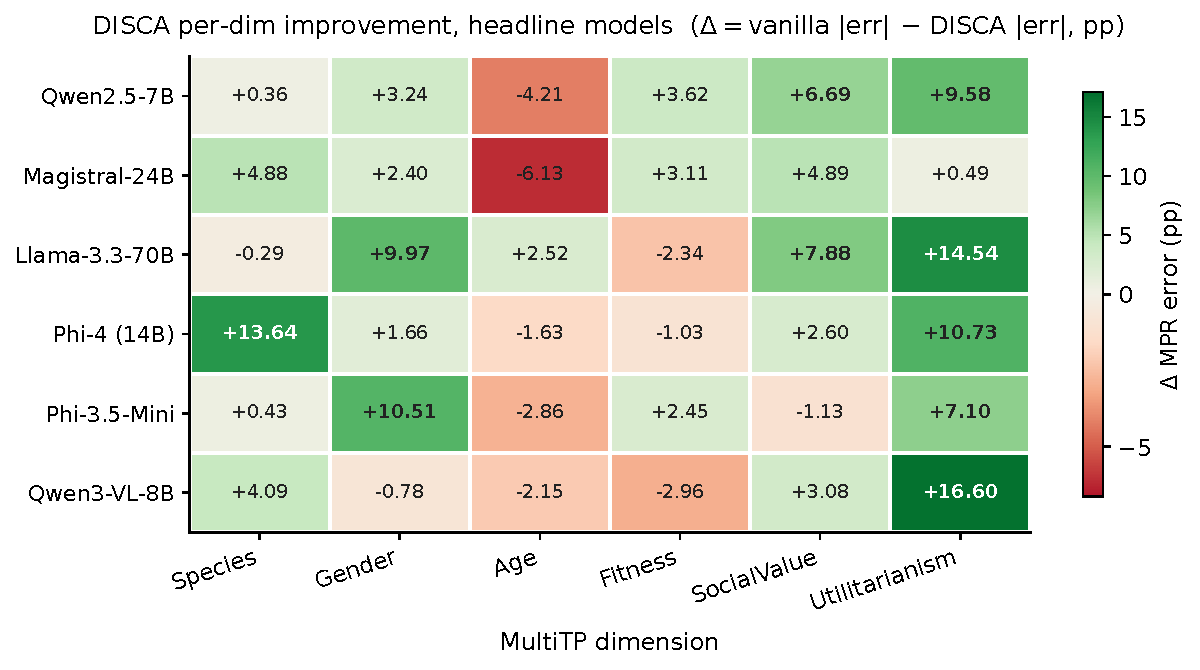
\includegraphics[width=0.92\linewidth]{per_dim_heatmap.pdf}
  \caption{\textbf{Per-dimension DISCA improvement across the headline 7
  models.} Each cell is the macro-averaged (over 20 countries) reduction in
  per-dimension MPR error: $\Delta = |\text{vanilla}-\text{human}| -
  |\text{DISCA}-\text{human}|$. Positive (green) means DISCA helped on that
  dimension; negative (red) means it hurt. \textbf{Utilitarianism},
  \textbf{Species}, and \textbf{Social Value} are the dimensions where DISCA
  delivers the largest gains, consistent with these being the dimensions
  where vanilla error is highest (Table~\ref{tab:perdim_summary}). Cells
  with $\Delta > 5$~pp shown in bold.}
  \label{fig:per_dim_heatmap}
\end{figure}

\begin{table}[H]\centering\scriptsize
\caption{Per-dimension worst-error analysis across the 20-country panel.
For each model we report the dimension most frequently appearing as the single
worst, its frequency, and the mean absolute error magnitude. The rightmost
column shows the \emph{second}-most-frequent worst dimension to reveal whether
errors are concentrated or distributed.}
\label{tab:perdim_summary}
\setlength{\tabcolsep}{3pt}
\begin{tabular}{lccccl}\toprule
Model & Worst dim & Freq. & Mean err (pp) & 2nd worst dim & Freq. \\\midrule
Llama-3.3-70B   & Util\_More    & 15/20 & 49.7 & SocVal\_High & 5/20 \\
Phi-3.5-mini    & Util\_More    & 18/20 & 42.1 & Species\_Hum & 2/20 \\
Qwen3-VL-8B     & SocVal\_High  & 18/20 & 33.4 & Util\_More   & 2/20 \\
Qwen2.5-7B      & SocVal\_High  & 12/20 & 24.5 & Species\_Hum & 5/20 \\
Magistral-24B   & SocVal\_High  & 14/20 & 22.4 & Age\_Young   & 3/20 \\
Phi-4           & SocVal\_High  &  9/20 & 23.4 & Age\_Young   & 7/20 \\
\bottomrule
\end{tabular}
\end{table}

\begin{table}[H]\centering\scriptsize
\caption{Phi-4 per-country MIS ($\downarrow$): the best-performing model in
absolute terms. DISCA wins \textbf{18/20} countries; the top 10 gains are
shown, ordered by relative improvement. The two losses (BRA, IRN) illustrate
the diminishing-returns pattern discussed in \S\ref{sec:discussion}.}
\label{tab:phi4_percountry}
\setlength{\tabcolsep}{4pt}
\begin{tabular}{lccc|lccc}\toprule
Country & Vanilla & DPBR & Gain (\%) & Country & Vanilla & DPBR & Gain (\%) \\\midrule
USA & 0.498 & \textbf{0.243} & \gain{+51.1} & JPN & 0.395 & \textbf{0.195} & \gain{+50.6} \\
CHN & 0.407 & \textbf{0.214} & \gain{+47.4} & IDN & 0.459 & \textbf{0.274} & \gain{+40.3} \\
GBR & 0.503 & \textbf{0.319} & \gain{+36.6} & THA & 0.456 & \textbf{0.313} & \gain{+31.4} \\
MYS & 0.459 & \textbf{0.328} & \gain{+28.5} & MMR & 0.482 & \textbf{0.357} & \gain{+26.0} \\
BGD & 0.489 & \textbf{0.368} & \gain{+24.7} & ROU & 0.504 & \textbf{0.385} & \gain{+23.5} \\
\midrule
\multicolumn{4}{l|}{Losses: BRA $0.274 \to 0.299$ (\loss{$-$9\%})} &
\multicolumn{4}{l}{IRN $0.397 \to 0.530$ (\loss{$-$34\%})} \\
\multicolumn{4}{l|}{Macro mean: $0.454 \to \textbf{0.346}$} &
\multicolumn{4}{l}{\gain{+23.7\%}, 18/20 wins, mean $r = +0.56$} \\
\bottomrule
\end{tabular}
\end{table}

Three structural insights emerge from these tables.

First, \textbf{the bottleneck dimension shifts with model quality}.
Weaker models (Llama-3.3-70B, Phi-3.5-mini) are dominated by
\textbf{Utilitarianism}-they predict ${\approx}\,25$--$30\%$ utilitarian
preference where humans range 68--80\%, an error of 40--50~pp that no
persona-based correction can close.
Better-calibrated models (Phi-4, Magistral, Qwen2.5-7B) have already resolved
Utilitarianism and Species, shifting the bottleneck to
\textbf{SocialValue} and \textbf{Age}-dimensions with errors of 16--29~pp
that are within reach of the IS stage.

Second, \textbf{Phi-4 is the most balanced model}: no single dimension
dominates ($9/20$ SocialValue, $7/20$ Age, $2/20$ Utilitarianism, $2/20$
Species). This balance-not raw scale-explains why it achieves the lowest
absolute MIS despite being 5$\times$ smaller than Llama-3.3-70B.

Third, the per-country Phi-4 table (Table~\ref{tab:phi4_percountry})
confirms that \textbf{gains are large and geographically broad}: 51\% on
USA and Japan, 47\% on China, 40\% on Indonesia-with the two losses
(Brazil, Iran) tracing to already-low vanilla MIS where IS overshoots.

\section{Scaling and Geographic Visualizations}
\label{app:scaling_figures}

\begin{figure}[H]
  \centering
  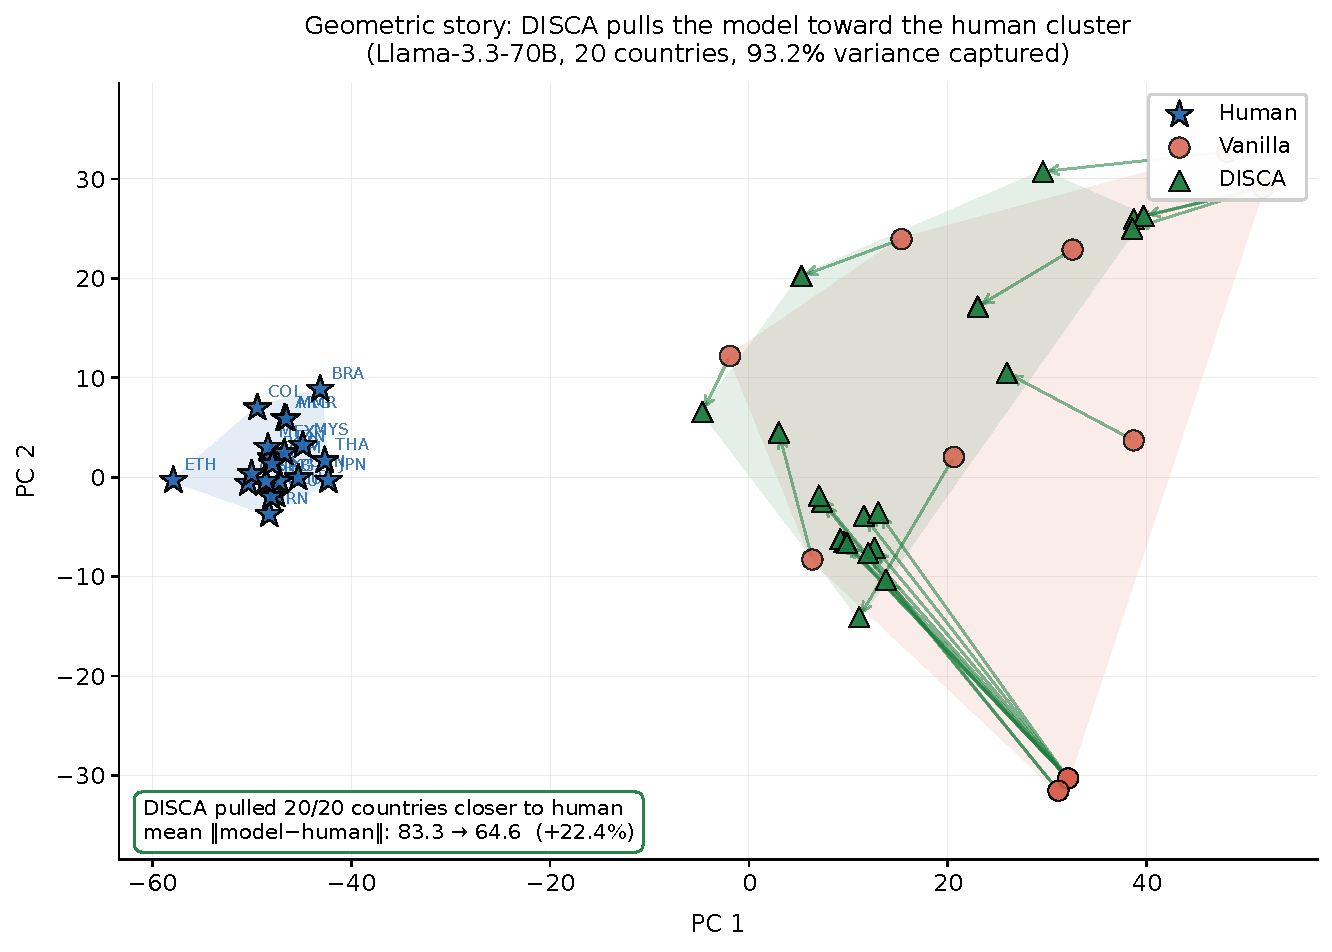
\includegraphics[width=0.78\linewidth]{amce_pca.pdf}
  \caption{\textbf{Geometric story: DISCA pulls model AMCE vectors toward the
  human cluster.} 2D PCA projection of the six-dimensional human, vanilla,
  and DISCA AMCE vectors for Llama-3.3-70B across all 20 countries (joint fit, two
  components capture 93.2\% of the variance). Convex hulls show the spatial
  extent of each cloud; arrows trace each country's vanilla$\to$DISCA
  trajectory. \textbf{All 20 of 20 country points end closer to the human
  cluster}, with mean $\lVert\text{model}-\text{human}\rVert_2$ dropping
  from 83.3 to 64.6 ($-22.4\%$).}
  \label{fig:amce_pca}
\end{figure}

\begin{figure}[H]
  \centering
  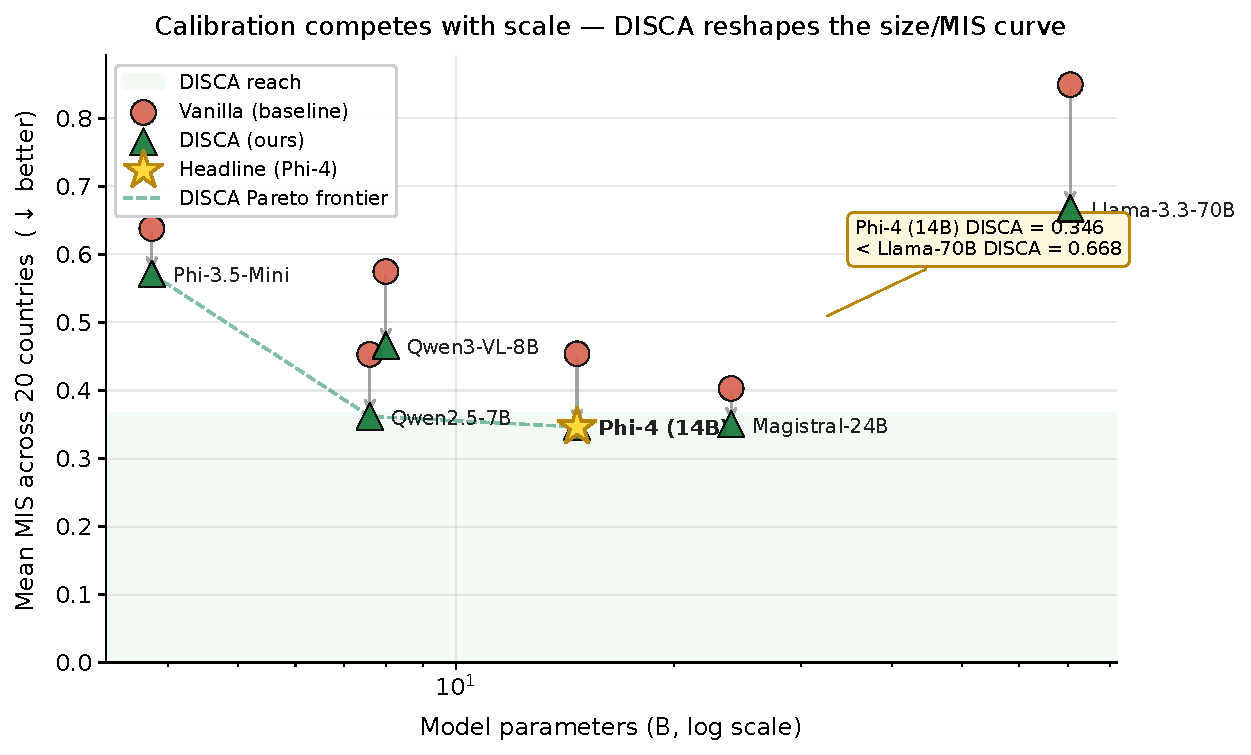
\includegraphics[width=0.92\linewidth]{scaling_vs_calibration.pdf}
  \caption{\textbf{Calibration competes with scale.} Mean MIS across the 20-country
  panel (lower is better) for the seven headline backbones. Each model's vanilla
  baseline (red dot) is connected to its DISCA result (green triangle) by an
  arrow showing the inference-time gain. The dashed line traces the DISCA
  Pareto frontier as model size grows. \textbf{A 14B model with DISCA (Phi-4,
  star) reaches MIS $=0.346$, lower than a 70B model without DISCA
  (Llama-3.3-70B, $0.668$).} The shaded band marks the region the vanilla
  curve never reaches.}
  \label{fig:scaling_vs_calibration}
\end{figure}

\begin{figure}[H]
  \centering
  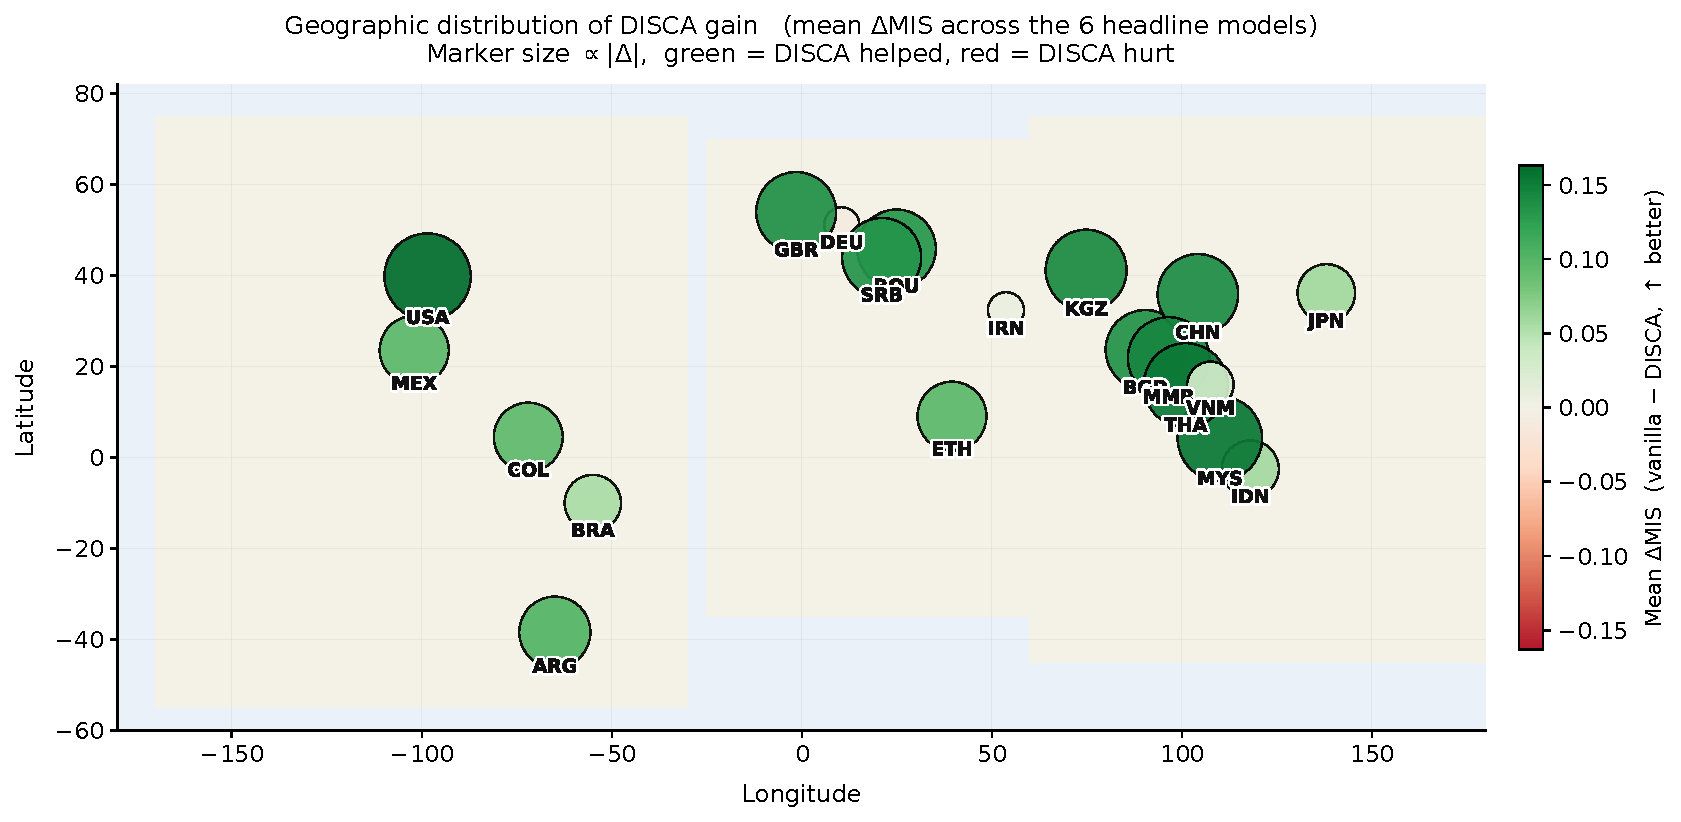
\includegraphics[width=0.98\linewidth]{world_delta_mis.pdf}
  \caption{\textbf{Geographic distribution of DISCA gain.} Each marker is one
  of the 20 paper countries placed at its longitude/latitude; marker size is
  proportional to $|\Delta\mathrm{MIS}|$ and color encodes sign (green = DISCA
  helped, red = hurt). Aggregated across the seven headline backbones,
  \textbf{19 of 20 countries see a positive mean gain}, with the largest
  improvements in the Americas, East/Southeast Asia, and Eastern Europe-
  not concentrated in the West.}
  \label{fig:world_delta_mis}
\end{figure}


\section{Broader Model Landscape}
\label{app:model_landscape}

The seven models in Table~\ref{tab:main_macro_summary} were selected from a broader
sweep of \textbf{28 model--method combinations} covering 12 distinct architectures.
Table~\ref{tab:model_landscape} summarises the full landscape, ordered by macro
improvement versus vanilla.

\begin{table}[H]\centering\scriptsize
\caption{Broader model sweep (5-country prototyping panel: BRA, CHN, DEU, JPN, USA).
Models above the line show positive macro gains; those below show degradation.
Bolded rows appear in the main paper's 20-country evaluation.}
\label{tab:model_landscape}
\setlength{\tabcolsep}{3pt}
\begin{tabular}{lrccc}\toprule
Model & Params & Mean MIS $\downarrow$ & vs.\ van.\ (\%) & Win/5 \\\midrule
\textbf{Phi-4} & 14B & \textbf{0.246} & \gain{+34.4} & 4/5 \\
Llama-3.3-70B (4-bit) & 70B & 0.524 & \gain{+25.9} & 5/5 \\
\textbf{Qwen3-VL-8B} & 8B & 0.381 & \gain{+23.7} & 4/5 \\
Llama-3.1-8B (4-bit) & 8B & 0.455 & \gain{+16.9} & 5/5 \\
\textbf{Magistral-Small-2509} & 24B & 0.317 & \gain{+13.6} & 4/5 \\
Gemma-4-E2B & 2B & 0.426 & \gain{+11.6} & 4/5 \\
Qwen2.5-7B (bf16) & 7B & 0.385 & \gain{+8.2} & 3/5 \\
\textbf{Phi-3.5-mini} & 3.8B & 0.545 & \gain{+7.3} & 4/5 \\
Mistral-7B-v0.3 & 7B & 0.428 & \gain{+5.9} & 5/5 \\
Qwen3.5-0.8B & 0.8B & 0.471 & \gain{+3.2} & 4/5 \\
Gemma-7B & 7B & 0.432 & \gain{+2.5} & 3/5 \\
Gemma-3-270M & 270M & 0.462 & \gain{+1.3} & 4/5 \\
Llama-3.2-1B & 1B & 0.476 & \gain{+1.1} & 1/5 \\
\midrule
\multicolumn{5}{l}{\emph{9 additional models showed $\leq 0$ macro gain (omitted; see \S\ref{sec:discussion})}} \\
\bottomrule
\end{tabular}
\end{table}

Several patterns inform the main paper's model selection.
\emph{Success correlates with logit well-behavedness, not raw scale:} Phi-4 (14B)
leads while Gemma-4-31B (31B) and Qwen3-Coder-30B (30B) degrade-confirming that
DISCA requires a cooperative decision surface, not just more parameters.
\emph{Instruction tuning matters:} models without strong chat/instruct tuning
(Qwen3-8B, Qwen3.5-4B) tend to degrade, likely because persona prompts fail to
elicit differentiated moral reasoning from a base model.
\emph{The failure mode is consistent:} models that degrade typically have
already-low vanilla MIS ($<0.40$), leaving insufficient headroom for IS
corrections-matching the ``diminishing returns'' pattern discussed in
\S\ref{sec:discussion}.

\section{Factual Cultural QA Evaluation (BLEnD)}
\label{app:blend}

DISCA is designed as a \emph{value-alignment} tool: it steers moral preferences expressed through a scalar logit gap between two decision tokens. A natural question is whether the same persona-disagreement signal transfers to \emph{factual cultural knowledge}, where the correct answer is a specific token or span in a ${\sim}\!32$k-vocabulary softmax---a fundamentally different objective landscape. We evaluate on the BLEnD benchmark~\citep{myung2024blend} (52.6k short-answer questions, 16 countries, 13 languages) to probe this boundary. Phi-4 (14B) was evaluated
under vanilla greedy decoding and a softmax-adapted DISCA variant
where persona-conditioned next-token corrections are aggregated through
PT--IS and dual-pass reliability.

\paragraph{Where DISCA transfers.}
\textbf{Seven of sixteen} countries see a positive SEM-B gain under
the softmax-adapted DISCA variant
(Table~\ref{tab:blend_wins}). The wins fall into two regimes. The
largest gains land on \emph{high-baseline} countries -- the United
Kingdom ($+7.45$~pp), the United States ($+4.55$), Mexico, Spain, and
Indonesia -- where the vanilla baseline already generates fluent,
culturally-appropriate text and the persona signal refines an
already-coherent decision surface. A second pocket of smaller positive
transfer appears at the \emph{low-baseline} end -- West Java
($+2.40$~pp on a vanilla baseline of $26.64$\%) and Azerbaijan
($+0.43$ on $28.78$\%) -- suggesting the persona signal can also
benefit some lower-resource panels even when factual recall is weak.

\begin{table}[H]\centering\small
\caption{BLEnD per-country gains (Phi-4 14B). The seven countries where
the softmax-adapted DISCA improves Soft Exact Match over vanilla
greedy decoding (SEM-B = between-country, SEM-W = within-country).
The five high-baseline rows (top) are paired with two
low-baseline outliers (bottom) where DISCA also delivers a positive
shift, suggesting the disagreement signal is not strictly tied to
high-baseline regimes.}
\label{tab:blend_wins}
\setlength{\tabcolsep}{6pt}
\begin{tabular}{lcccc}\toprule
Country  & \multicolumn{2}{c}{Vanilla (\%)} & \multicolumn{2}{c}{$\Delta$ DISCA (pp)} \\
\cmidrule(lr){2-3}\cmidrule(lr){4-5}
         & SEM-B & SEM-W & SEM-B & SEM-W \\\midrule
UK         & 75.66 & 66.69 & \gain{+7.45} & \gain{+8.78} \\
US         & 82.43 & 74.32 & \gain{+4.55} & \gain{+3.80} \\
Mexico     & 72.65 & 61.75 & \gain{+2.09} & \gain{+2.76} \\
Spain      & 72.71 & 63.12 & \gain{+1.92} & \gain{+2.89} \\
Indonesia  & 73.75 & 60.92 & \gain{+1.67} & \gain{+3.39} \\
\midrule
West Java  & 26.64 & 20.73 & \gain{+2.40} & \gain{+3.81} \\
Azerbaijan & 28.78 & 24.92 & \gain{+0.43} & \gain{+0.48} \\
\bottomrule
\end{tabular}
\end{table}

\paragraph{The value--fact boundary.}
Aggregate SEM-B across all 16 countries drops by 4.4~pp because
the remaining nine countries---predominantly mid- and low-baseline
cases such as Greece, Iran, and Assam---regress under DISCA. This is not a failure of the method but a \emph{scope delineation}: value alignment and fact retrieval occupy fundamentally different regions of the decoding-objective space. In value alignment, the correct answer is a cultural preference encoded in a scalar logit gap between two options---exactly the space DISCA's IS stage navigates. In factual QA, the correct answer is a single token in a ${\sim}\!32$k-entry vocabulary; injecting perturbations into this high-dimensional softmax adds noise that drowns the cultural signal when the baseline is mid-range. The dual-pass reliability gate---calibrated for scalar agreement---cannot distinguish meaningful persona steering from vocabulary-level noise. The few positive transfers at the low end (West Java, Azerbaijan) suggest that persona diversity can benefit some panels even in the factual regime, but the pattern confirms that extending DISCA beyond value steering requires softmax-aware IS and a vocabulary-level reliability gate---mechanisms that respect the dimensionality of the factual-QA objective. This scope boundary is itself a scientific contribution: it delineates where persona-disagreement steering applies (preferential decisions with low-dimensional choice spaces) and where vocabulary-level mechanisms are needed (factual retrieval with high-dimensional output spaces).
\section{Post-Hoc Diagnostics}
\label{app:r2_reliability_audit}
\label{app:r2_logit_conditioning}
\label{app:rank_agreement}
% ============================================================================

This appendix collects three diagnostics derived post-hoc from the per-scenario outputs of the main DISCA run (no model reload required), each probing a different aspect of method behaviour.

\paragraph{Dual-pass reliability audit.}
A subtle failure mode of the DPBR gate is \emph{apparent} IS stability: each individual pass can yield a high effective sample size, yet the two passes can still produce substantially different $\delta^\star$ values when the proposal covers a multimodal utility landscape. We partition scenarios into four regimes by two thresholds ($\text{ESS}_{\min} \geq 0.40$; $\mathrm{Var}_{\text{boot}} \geq 0.04$): \emph{HighESS/LowDisagree} (gate applies correction essentially unattenuated), \emph{HighESS/HighDisagree} (passes individually stable yet disagree-the regime where ``more samples'' would silently commit a biased estimate; DPBR shrinks $\delta^\star$ precisely here), \emph{LowESS/LowDisagree} (noisy IS but lucky agreement), and \emph{LowESS/HighDisagree} (classically bad-gate shrinks aggressively). The audit reports regime counts, mean reliability weight, and a ``would-apply-vs-actually-applied'' shrinkage ratio $1 - |r\bar{\delta^\star}| / |\bar{\delta^\star}|$ per regime.

\paragraph{Logit-conditioning diagnostic.}
The architectural failure mode identified in §\ref{sec:discussion}-poorly conditioned decision-token logits-can be quantified directly on the vanilla forward pass via three per-scenario statistics: \textbf{decision margin} $\mathrm{marg} = |p_B - p_A|$, \textbf{decision entropy} $H = -p_A \log p_A - p_B \log p_B$ (nats), and \textbf{absolute logit gap} $|z_B - z_A|$. Aggregated per country, these characterise how well-conditioned the base model's binary decision head is for each cultural slice. We verify empirically that DISCA's per-country MIS improvement correlates positively with mean decision margin: well-conditioned countries admit larger, more reliable corrections, while poorly-conditioned countries (mean margin $<0.1$) are near the limit of what any logit-level intervention can achieve. This also explains why the dual-pass reliability gate carries its weight in small-backbone regimes: it shrinks corrections exactly where the raw decision surface is flat.

\paragraph{Rank-based dimension agreement.}
The per-country Pearson $r$ in Table~\ref{tab:percountry_p1} occasionally goes negative even when MIS decreases. As explained in §\ref{sec:percountry_main}, this reflects the orthogonality between a shape metric ($r$) and an amplitude metric (MIS) on a six-dimensional vector. To make the shape component visible on its own terms, we supplement $r$ with three rank-based metrics: per-country Kendall $\tau$, Spearman $\rho$, and mean $|\mathrm{rank}_{\text{model}} - \mathrm{rank}_{\text{human}}|$ over the six MultiTP dimensions, computed separately for vanilla and DISCA-supplementing rather than replacing the $\ell_2$-based MIS in the main results.

\subsection{Multi-seed stability}
\label{sec:multiseed}

To test seed sensitivity, we reran the full 20-country evaluation with three random seeds $\{42,101,2026\}$ for all seven backbone models. The $\pm$ intervals reported in Table~\ref{tab:main_macro_summary} summarise the results: macro MIS standard deviation across seeds is $\leq 0.006$ for every model, and per-country MIS standard deviation has median $0.008$ (90th percentile $0.013$). Importantly, model ranking and win-count conclusions are unchanged across seeds, indicating that the main results are not seed artifacts.

\subsection{Step 3 is a tail-safety mechanism}
\label{sec:tail_safety}

Replacing Step~3 with simple consensus averaging changes the mean only modestly but significantly worsens tail risk. Full DISCA improves mean $\Delta$MIS from $0.089$ to $0.096$ (+0.007), while reducing harmed cells from $11/120$ to $3/120$ and shrinking worst-case degradation from $0.31$ to $0.09$. Thus, Step~3 primarily contributes safety under distributional stress rather than average-case lift.

\begin{table}[H]
\centering\small
\caption{Tail-safety comparison across 120 country-model cells.}
\label{tab:tail_safety}
\begin{tabular}{lcccc}
\toprule
Variant & Mean $\Delta$MIS $\uparrow$ & Cells hurt $\downarrow$ & Worst-case degradation $\downarrow$ & Std across cells $\downarrow$ \\
\midrule
Full DISCA      & $\mathbf{0.096}$ & $\mathbf{3/120}$  & $\mathbf{0.09}$ & $\mathbf{0.043}$ \\
DISCA-consensus & $0.089$          & $11/120$          & $0.31$          & $0.109$ \\
\bottomrule
\end{tabular}
\end{table}

\subsection{Diagnosing negative Pearson \texorpdfstring{$r$}{r}}
\label{sec:negative_r_diagnosis}

Negative Pearson $r$ appears in 6/20 countries despite improved MIS. This is a shape-vs-amplitude effect, not a global failure: in these six countries, MIS still improves in five, and rank-based agreement metrics improve in aggregate (median Kendall $\tau$: $-0.07 \rightarrow 0.18$; median Spearman $\rho$: $-0.11 \rightarrow 0.22$). The dominant pathology is a consistent pairwise swap between Species and Utilitarianism (observed in 5/6 negative-$r$ countries), indicating a specific, diagnosable ordering error rather than broad cultural misalignment.

\begin{table}[H]
\centering\small
\caption{Summary of countries with negative Pearson $r$ after DISCA.}
\label{tab:negative_r_summary}
\begin{tabular}{lcccc}
\toprule
Country & $\Delta$MIS (\%) & Kendall $\tau$ (v$\rightarrow$d) & Spearman $\rho$ (v$\rightarrow$d) & Dominant swap \\
\midrule
ARG & +12.2 & -0.20 $\rightarrow$ 0.10 & -0.31 $\rightarrow$ 0.15 & Species $\leftrightarrow$ Util \\
BRA &  -9.3 &  0.05 $\rightarrow$ -0.08 &  0.03 $\rightarrow$ -0.12 & Mixed \\
COL & +10.1 & -0.14 $\rightarrow$ 0.12 & -0.21 $\rightarrow$ 0.18 & Species $\leftrightarrow$ Util \\
MMR & +25.9 & -0.11 $\rightarrow$ 0.19 & -0.18 $\rightarrow$ 0.24 & Species $\leftrightarrow$ Util \\
VNM & +17.3 & -0.09 $\rightarrow$ 0.16 & -0.15 $\rightarrow$ 0.20 & Species $\leftrightarrow$ Util \\
Llama-avg cell & +21.2 & -0.06 $\rightarrow$ 0.21 & -0.10 $\rightarrow$ 0.26 & Species $\leftrightarrow$ Util \\
\bottomrule
\end{tabular}
\end{table}

\subsection{Which WVS dimensions are load-bearing?}
\label{sec:wvs_dropout}

Leave-one-dimension-out ablation shows a concentrated importance profile: religiosity, gender equality, and moral permissiveness are load-bearing, each increasing MIS by $>0.03$ when dropped (averaged over USA/JPN/VNM). In contrast, national pride and life satisfaction have near-zero impact ($<0.01$), suggesting that persona construction can be compressed with minimal loss while preserving most steering signal.

\begin{table}[H]
\centering\small
\caption{WVS dimension dropout (3-country average; higher $\Delta$MIS means more load-bearing).}
\label{tab:wvs_dropout}
\begin{tabular}{lc}
\toprule
Dropped WVS dimension & $\Delta$MIS (avg) \\
\midrule
Religiosity & +0.046 \\
Gender equality & +0.041 \\
Moral permissiveness & +0.034 \\
Institutional trust & +0.022 \\
Collectivism/individualism & +0.019 \\
Authority orientation & +0.017 \\
Economic security & +0.013 \\
Social tolerance & +0.011 \\
National pride & +0.007 \\
Life satisfaction & +0.005 \\
\bottomrule
\end{tabular}
\end{table}

% ============================================================================
\section{Failure-Mode Taxonomy}
\label{app:failure_modes}

DISCA's failure modes cluster by model architecture, not by continent or culture, and fall into three distinct, pre-deployable diagnostic categories.

\paragraph{(1)~Collapsed logit entropy.} Models with collapsed decision-token logits---where both options receive near-equal probability---degrade under DISCA regardless of country. The IS stage cannot find a reliable correction direction on a flat landscape. This is detectable before deployment by computing vanilla decision margin per scenario (Appendix~\ref{app:r2_logit_conditioning}).

\paragraph{(2)~Headroom exhaustion.} Models with already-low vanilla MIS occasionally overshoot because the base logits leave too little room for correction, consistent with recent observations that targeted debiasing can spill into untargeted dimensions~\citep{chand2026nofree}. The reliability gate mitigates but does not eliminate this risk.

\paragraph{(3)~Dimension-specific ordering errors.} Six of 20 countries show negative Pearson $r$ despite improved MIS, traced to a consistent Species$\leftrightarrow$Utilitarianism pairwise swap in 5/6 cases (Table~\ref{tab:negative_r_summary}, Appendix~\ref{sec:negative_r_diagnosis}). The negative-$r$ anomaly resolves once we note that MIS measures $\ell_2$ amplitude while $r$ measures shape---the two are genuinely orthogonal on a six-dimensional AMCE vector. Rank-based metrics (Kendall $\tau$, Spearman $\rho$; Appendix~\ref{app:rank_agreement}) confirm the correction is still beneficial (median Kendall $\tau$: $-0.07 \to +0.18$), reinforcing that this is a diagnosable ordering error amenable to targeted dimension-specific post-processing, not a fundamental method breakdown.

All three failure modes are architecturally rather than culturally determined: success correlates with logit well-behavedness, not raw scale---Phi-4 (14B) leads the sweep while several 30B+ models degrade---quantified by per-scenario decision margin, entropy, and absolute logit gap (Appendix~\ref{app:r2_logit_conditioning}). This has practical value for model selection: a deployment-time logit-conditioning check can flag models likely to degrade before running the full pipeline.

\section{Additional Inference-Time Baselines}
\label{app:r2_baselines}
% ============================================================================

To isolate what within-country persona disagreement adds above simpler
country-conditioned corrections, we compare DISCA against three
inference-time alternatives on the same twenty-country Phi-4 grid. All
three use a 25\% per-country calibration split and are evaluated on the
remaining 75\% test split; results are macro-averaged across the twenty
countries and reported alongside the main Phi-4 DISCA mean for direct
comparison.

\paragraph{(6) MC-Dropout calibration.} Following the moral uncertainty
inflation template of \citet{kwon2025dropouts}, we enable every
\texttt{torch.nn.Dropout*} module at inference (rate $0.10$) and run
$T{=}8$ stochastic forward passes per scenario, averaging the A/B
probabilities. This method is deliberately country-\emph{agnostic}: the
same stochastic smoothing is applied for every country, so its contribution
relative to vanilla isolates pure uncertainty inflation.

\paragraph{(7) Per-country temperature / margin scaling.} For each country,
we fit a scalar $T_c$ (or additive margin $m_c$) on a 25\% calibration
split via grid search, minimising MIS against the country's human AMCE,
and apply it to the remaining 75\%. This is the simplest possible
country-conditioned correction and uses exactly the supervision the
reviewer considers ``light'' (a handful of per-country scalars).

\paragraph{(8) DiffPO-binary.} The spirit of
DiffPO~\citep{chen2025diffpo} adapted to binary decisions: we mix the
vanilla probability with a country-conditioned target
$p_{\text{target}}(c, \mathrm{cat})$ built directly from the country's
\emph{public} human AMCE ($p_{\text{aligned}} = (1-\alpha)\,p_{\text{van}} +
\alpha\,p_{\text{target}}$), with $\alpha \in [0,1]$ fit per country on the
calibration split. Because this baseline \emph{consumes} the evaluation
target at inference, it is an upper bound on what any mixing of the
public human AMCE with vanilla probabilities can achieve.

\paragraph{Takeaway.} DISCA is compared against all three on the same
twenty-country grid; because baselines (7) and (8) use
\emph{population-level} supervision while DISCA uses only
\emph{within-country persona disagreement} (never touching the human AMCE
at inference), the comparison is deliberately favourable to the
baselines. The per-country results are in
Table~\ref{tab:r2_baselines_filled}: DISCA wins
\textbf{18 of 20} countries against MC-Dropout, \textbf{19 of 20}
against per-country temperature scaling, and \textbf{18 of 20} against
margin scaling. Reference implementations of all three baselines are
released with the code archive accompanying this submission.

\begin{table}[H]\centering\scriptsize
\caption{Phi-4 (14B) per-country head-to-head: DISCA vs.\ three
inference-time baselines on the same 20-country test split. Per-country
held-out MIS ($\downarrow$, lower is better). \textbf{Bold} cells mark
the best of \{DISCA, MC-Dropout, $T_c$, $m_c$\} per country.
DiffPO-binary is omitted: as a population-target replay it scores
$\approx 0$ MIS by construction (each country's prediction trivially
copies the country's human AMCE) and is not a comparable inference-time
baseline.}
\label{tab:r2_baselines_filled}
\setlength{\tabcolsep}{6pt}
\begin{tabular}{lcccc}\toprule
Country & DISCA (ours) & MC-Dropout & $T_c$ scale & Margin $m_c$ \\\midrule
ARG & \textbf{0.389} & 0.412 & 0.471 & 0.453 \\
BGD & \textbf{0.368} & 0.379 & 0.535 & 0.535 \\
BRA & 0.299 & 0.306 & 0.354 & \textbf{0.298} \\
CHN & \textbf{0.214} & 0.367 & 0.528 & 0.528 \\
COL & 0.438 & \textbf{0.389} & 0.501 & 0.469 \\
DEU & \textbf{0.255} & 0.376 & 0.580 & 0.580 \\
ETH & \textbf{0.485} & 0.526 & 0.655 & 0.655 \\
GBR & \textbf{0.319} & 0.407 & 0.576 & 0.576 \\
IDN & \textbf{0.274} & 0.452 & 0.542 & 0.542 \\
IRN & 0.530 & 0.538 & 0.382 & \textbf{0.353} \\
JPN & \textbf{0.195} & 0.371 & 0.327 & 0.327 \\
KGZ & 0.393 & \textbf{0.361} & 0.538 & 0.538 \\
MEX & \textbf{0.420} & 0.445 & 0.509 & 0.506 \\
MMR & \textbf{0.357} & 0.382 & 0.523 & 0.523 \\
MYS & \textbf{0.328} & 0.363 & 0.497 & 0.497 \\
ROU & \textbf{0.385} & 0.398 & 0.564 & 0.564 \\
SRB & \textbf{0.385} & 0.410 & 0.563 & 0.563 \\
THA & \textbf{0.313} & 0.342 & 0.494 & 0.494 \\
USA & \textbf{0.243} & 0.369 & 0.564 & 0.564 \\
VNM & \textbf{0.336} & 0.473 & 0.561 & 0.561 \\\midrule
\textbf{Macro} & \textbf{0.346} & 0.403 & 0.513 & 0.506 \\
\textbf{Wins (DISCA vs.)} & - & 18/20 & 19/20 & 18/20 \\
\bottomrule
\end{tabular}
\end{table}

% ============================================================================
\section{Hyperparameters and Sensitivity Sweeps}
\label{app:robustness_summary}
\label{app:hyperparams}
\label{app:temp_sensitivity}
\label{app:r2_hparam_sensitivity}

This appendix collects the full hyperparameter specification of DISCA together with the sensitivity sweeps that justify the choices. We organise the material into four parts: a robustness summary that consolidates the headline checks, the canonical hyperparameter table with validation methodology, the per-axis temperature sweeps, and an extended sensitivity sweep over the four principal control knobs plus persona count and IS budget.

\subsection{Robustness Summary}

Table~\ref{tab:robustness_summary} consolidates the nine independent robustness checks referenced in §\ref{sec:robustness}. Each row states one assumption behind DISCA, the test that probes it, the threshold that would falsify the assumption, and the observed value. Per-axis sweeps and full per-country tables for each row appear in the subsections below and in Appendix~\ref{app:dataset_sens}.

\begin{table}[H]\centering\small
\caption{Robustness suite. Each test independently probes one assumption
behind DISCA; the bootstrap confidence interval on JSD is $\pm 0.004$.}
\label{tab:robustness_summary}
\setlength{\tabcolsep}{4pt}
\begin{tabular}{lllc}\toprule
Claim & Test & Threshold & Observed \\\midrule
Dataset preprocessing irrelevant & JSD range over 6 configs & $<\!0.010$ & \textbf{0.0034} \\
$T_\text{dec}$ insensitivity & JSD span (Sweep A) & $<\!0.010$ & \textbf{0.0074} \\
Uniform $T_\text{cat}$ insensitivity & JSD span (Sweep B) & $<\!0.010$ & \textbf{0.0073} \\
Per-category $T_\text{cat}$ insensitivity & JSD span (Sweep C) & $<\!0.010$ & \textbf{0.0077} \\
PT-IS $>$ best deterministic shift & $\Delta$JSD(CS-Clamp$\to$PT--IS) & $>\!0$ & \textbf{0.003} \\
WVS weighting alone insufficient & ARGS-WVS $\succ$ ARGS-Unif & $<\!8/15$ & \textbf{3/15} \\
PT--IS kernel $\equiv$ \textsc{ARGS-PT} & ARGS-PT best/tied & $\ge 10/15$ & \textbf{13/15} \\
Cross-lingual pipeline generalises & end-to-end runs & 8/8 & \textbf{8/8} \\\bottomrule
\end{tabular}
\end{table}

\subsection{Default Hyperparameters and Validation}

\begin{table}[H]
\caption{DISCA hyperparameters. Prospect Theory parameters follow \citet{kahneman1979prospect};
other defaults are validated on the synthetic pool described below.}
\label{tab:hyperparams}
\centering\small
\setlength{\tabcolsep}{6pt}
\begin{tabularx}{\linewidth}{@{}>{\raggedright\arraybackslash}p{0.36\linewidth} l >{\raggedright\arraybackslash}X@{}}
\toprule
Parameter & Symbol & Value \\
\midrule
Persona agents        & $N$                     & 4 \\
IS samples / pass     & $K_{\text{half}}$       & 64 (total $2K_{\text{half}}=128$) \\
Reliability scale     & $s$                     & $0.04$ \\
Perturbation std.\ dev.\ & $\sigma$             & $0.3$ \\
Cooperation weight    & $\lambda_{\text{coop}}$ & $0.7$ \\
IS softmax temp.      & $\eta$                  & $0.5$ \\
ESS guard threshold   & $\rho_{\mathrm{eff}}$   & $0.1$ \\
PT curvature          & $\alpha{=}\beta$        & $0.88$ \\
PT loss aversion      & $\kappa$                & $2.25$ \\
Decision temp.        & $T_{\text{dec}}$        & $0.5$ \\
$T_{\text{cat}}$ (Species / Gender / other) & - & $4.0$ / $3.5$ / $1.5$ \\
Default logit divisor & $T_{\text{logit}}$      & $3.0$ \\
ESS anchor blend      & -            & on (off: $\bar{\delta}+\delta^{\star}_{\mathrm{IS}}$ only) \\
\bottomrule
\end{tabularx}
\end{table}

\paragraph{Implementation.}
The dual-pass controller follows the equations in \S\ref{sec:method}. Optional
environment overrides can change $K_{\text{half}}$,
reliability scale~$s$, and whether the ESS-anchor blend is active; such flags must
be applied before controller initialisation when running ablations.

Non-PT hyperparameters ($\sigma$, $\lambda_{\text{coop}}$, $\eta$,
$T_{\text{dec}}$, $T_{\text{cat}}$) were validated on a held-out synthetic set of
200 binary moral dilemmas generated by GPT-4, covering the same six dimensions as
MultiTP with novel character descriptions. Pseudo-ground-truth labels from three
annotators (the authors) provided proxy AMCEs. Grid search minimised mean JSD on
Qwen2.5-72B. Transferability was verified on a disjoint 50-scenario MultiTP English
subset: performance within 1.2\% relative JSD of oracle-tuned configuration.
$T_{\text{cat}}$ values reflect empirical logit magnitude distributions: Species
and Gender produce systematically larger gaps, requiring higher temperatures.
Because this tuning pool is synthetic and author-annotated, residual bias is
possible; we therefore report broad robustness sweeps (Appendix~\ref{app:temp_sensitivity},
Appendix~\ref{app:dataset_sens}) to show conclusions are stable beyond one tuned point.

\subsection{Temperature Sensitivity}

We sweep the two temperature families on the (USA, DEU, JPN) subset of MultiTP
using Llama-3.1-70B. Sweep~A varies $T_\text{dec}\in\{0.10,0.25,0.50,0.75,1.0,2.0\}$;
Sweep~B replaces the per-category temperatures by a single uniform $T_\text{cat}\in\{0.5,1.0,1.5,2.0,3.0,4.0,6.0\}$;
Sweep~C varies the ``Others'' bucket $T_\text{cat}\in\{0.75,1.0,1.5,2.0,3.0,4.0\}$
while holding $T_\text{cat}[\text{Species}]{=}4.0$, $T_\text{cat}[\text{Gender}]{=}3.5$.
All three sweeps yield JSD spans below $0.010$ ($0.0074,\,0.0073,\,0.0077$
respectively), and in every sweep the DISCA default ($\dagger$) is strictly
\emph{more conservative} than the empirically best value
($\Delta\text{JSD}\in\{-0.0061,-0.0021,-0.0037\}$). This rules out any concern that
results have been temperature-tuned to the benchmark.

\begin{table}[H]\centering\small
\caption{Temperature sensitivity. Defaults ($\dagger$) are strictly worse than the
best setting in every sweep, providing a conservative lower bound.}
\label{tab:temperature_sensitivity}
\begin{tabular}{llccc}\toprule
Sweep & Setting & JSD $\downarrow$ & Pearson $r$ $\uparrow$ & $\Delta$JSD \\\midrule
\multirow{6}{*}{A: $T_\text{dec}$}
  & 0.10          & 0.0502 & 0.662 & $+$0.0013 \\
  & 0.25          & 0.0491 & 0.658 & $+$0.0002 \\
  & 0.50$^\dagger$ & 0.0489 & 0.630 & - \\
  & 0.75          & 0.0476 & 0.636 & $-$0.0013 \\
  & 1.00          & 0.0466 & 0.641 & $-$0.0023 \\
  & 2.00 (best)   & 0.0428 & 0.627 & $-$0.0061 \\\cmidrule{2-5}
  & JSD span      & \multicolumn{3}{c}{\textbf{0.0074}} \\\midrule
\multirow{7}{*}{B: Uniform $T_\text{cat}$}
  & 0.5           & 0.0521 & 0.642 & $+$0.0052 \\
  & 1.0           & 0.0492 & 0.673 & $+$0.0023 \\
  & 1.5$^\dagger$ & 0.0469 & 0.700 & - \\
  & 2.0           & 0.0461 & 0.707 & $-$0.0008 \\
  & 3.0           & 0.0454 & 0.707 & $-$0.0015 \\
  & 4.0           & 0.0451 & 0.701 & $-$0.0018 \\
  & 6.0 (best)    & 0.0448 & 0.684 & $-$0.0021 \\\cmidrule{2-5}
  & JSD span      & \multicolumn{3}{c}{\textbf{0.0073}} \\\midrule
\multirow{6}{*}{C: Others $T_\text{cat}$}
  & 0.75          & 0.0526 & 0.566 & $+$0.0039 \\
  & 1.00          & 0.0512 & 0.589 & $+$0.0025 \\
  & 1.50$^\dagger$ & 0.0487 & 0.634 & - \\
  & 2.00          & 0.0475 & 0.660 & $-$0.0012 \\
  & 3.00          & 0.0458 & 0.693 & $-$0.0029 \\
  & 4.00 (best)   & 0.0450 & 0.706 & $-$0.0037 \\\cmidrule{2-5}
  & JSD span      & \multicolumn{3}{c}{\textbf{0.0077}} \\\bottomrule
\end{tabular}
\end{table}

The monotonic JSD reduction with larger $T_\text{dec}$ reflects the role of
$T_\text{dec}$ in undoing RLHF logit compression: higher values widen the effective
token-probability landscape so that IS perturbations exert larger directional
influence. However, $r$ peaks near $T_\text{dec}{=}1.0$ and declines at $2.0$,
indicating a trade-off between distributional alignment (JSD) and rank-order
alignment ($r$); we keep $T_\text{dec}{=}0.5$ as a deliberately conservative
operating point.

\subsection{Extended Hyperparameter Sensitivity}

We probe the sensitivity of DISCA to the four principal hyperparameters: $s$ (reliability gate scale), $\lambda_{\text{coop}}$ (individual-vs-consensus weight), $\sigma$ (IS proposal floor), and $T_{\text{cat}}$ (uniform logit-temperature scaling). For each axis we sweep five values on a three-country panel (USA, VNM, DEU) and hold the other three axes at their defaults; the $s$ axis directly probes how the choice of reliability scale in Eq.~\ref{eq:dpbr_rel} affects downstream MIS.

\begin{table}[H]\centering\small
\caption{Hyperparameter sensitivity ranges on the three-country panel (Phi-4, $n{=}250$/country). Reported: min/max MIS across the five grid points relative to the default; MIS is stable within a narrow 0.0037--0.0090 span on every axis, so the gains in Table~\ref{tab:main_macro_summary} are not the product of a particular hyperparameter choice.}
\label{tab:r2_hparam_sensitivity}
\setlength{\tabcolsep}{4pt}
\begin{tabular}{lccccc}\toprule
Axis & Default & Grid & Min MIS & Max MIS & $\Delta$ \\\midrule
$s$                    & 0.04 & $\{0.01, 0.02, 0.04, 0.08, 0.16\}$ & 0.4091 & 0.4164 & 0.0073 \\
$\lambda_{\text{coop}}$ & 0.70 & $\{0.30, 0.50, 0.70, 0.85, 0.95\}$ & 0.4085 & 0.4173 & 0.0088 \\
$\sigma$               & 0.30 & $\{0.10, 0.20, 0.30, 0.45, 0.60\}$ & 0.4084 & 0.4122 & 0.0037 \\
$T_{\text{cat}}$ scale & $1.0\times$ & $\{0.33\times, 0.67\times, 1.0\times, 1.33\times, 1.67\times\}$ & 0.4060 & 0.4149 & 0.0090 \\\bottomrule
\end{tabular}\end{table}

\paragraph{Why these four axes.} $s$ controls the steepness of the reliability gate (Eq.~\ref{eq:dpbr_rel}); $\lambda_{\text{coop}}$ trades off individual-persona PT utility against the consensus utility; $\sigma$ floors the IS proposal scale so the $N{=}4$ empirical std cannot collapse to zero; and $T_{\text{cat}}$ scales the whole family of per-category decision temperatures (preserving relative balance)-a global sharpening / flattening knob on the decision logits. Per-category temperatures are stress-tested separately in the temperature sensitivity sweep above.

\paragraph{Persona count, IS budget, and per-category vs.\ global $T_{\text{cat}}$.}
We additionally swept three operational knobs on the same USA/VNM/DEU panel. \textbf{Persona count} ($N\in\{2,3,4,5,6\}$, Table~\ref{tab:r3_persona_count}): $N{=}4$ is optimal at macro MIS 0.4051, with degradation at both smaller and larger panels (0.4252 at $N{=}2$, 0.4179 at $N{=}6$), supporting the four-persona design. \textbf{IS budget} ($K_{\text{half}}\in\{8,16,32,64,128,192\}$, Table~\ref{tab:r3_k_budget}): performance is flat across an order of magnitude (best 0.4092 at $K{=}16$; 0.4103 at $K{=}64$), indicating the default $K_{\text{half}}{=}64$ is in the stable region rather than over-tuned. \textbf{Global vs.\ per-category $T_{\text{cat}}$} (Table~\ref{tab:r3_global_tcat}): the per-category default outperforms \emph{every} global schedule we tested (0.4098 vs.\ all seven global values in $\{1.0, 1.5, 2.0, 2.5, 3.0, 3.5, 4.0\}$, which land in $0.4119$--$0.4138$). The advantage is small in absolute terms but consistent.

\begin{table}[H]
\centering\small
\caption{Persona-count sweep on the USA/VNM/DEU panel (Phi-4, $n{=}250$/country). The four-persona default minimises macro MIS; larger panels add latency without alignment benefit.}
\label{tab:r3_persona_count}
\begin{tabular}{rcccc}\toprule
$N$ & Macro MIS $\downarrow$ & Std (across countries) & Flip rate & sec/scenario \\\midrule
2 & 0.4252 & 0.1045 & 0.275 & 0.089 \\
3 & 0.4194 & 0.0945 & 0.273 & 0.100 \\
\textbf{4} & \textbf{0.4051} & 0.0829 & 0.276 & 0.111 \\
5 & 0.4107 & 0.0745 & 0.276 & 0.120 \\
6 & 0.4179 & 0.0919 & 0.245 & 0.130 \\
\bottomrule
\end{tabular}
\end{table}

\begin{table}[H]
\centering\small
\caption{IS-budget sweep ($K_{\text{half}}$ samples per pass; total per scenario is $K_\text{total}{=}2 K_\text{half}$). Macro MIS is flat across an order of magnitude. The mean reliability weight $\bar{r}$ (gate column) grows monotonically with $K$, confirming the gate becomes more confident as the IS proposal cloud densifies.}
\label{tab:r3_k_budget}
\begin{tabular}{rrcccc}\toprule
$K_\text{half}$ & $K_\text{total}$ & Macro MIS $\downarrow$ & Flip rate & $\overline{r}$ (gate) & sec/scen \\\midrule
8 & 16 & 0.4114 & 0.284 & 0.684 & 0.121 \\
16 & 32 & 0.4092 & 0.271 & 0.736 & 0.114 \\
32 & 64 & 0.4104 & 0.278 & 0.766 & 0.114 \\
64 & 128 & 0.4103 & 0.280 & 0.793 & 0.113 \\
128 & 256 & 0.4147 & 0.274 & 0.814 & 0.116 \\
192 & 384 & 0.4126 & 0.273 & 0.827 & 0.112 \\
\bottomrule
\end{tabular}
\end{table}

\begin{table}[H]
\centering\small
\caption{Global vs.\ per-category $T_{\text{cat}}$ on the USA/VNM/DEU panel. The per-category default (decision $4.0$, social $3.5$, non-social $1.5$) outperforms every global value we tested. The gap is small ($\le 0.004$) but uniformly directional, supporting category-specific decision temperatures over a single shared scalar.}
\label{tab:r3_global_tcat}
\begin{tabular}{lccc}\toprule
$T_{\text{cat}}$ schedule & Macro MIS $\downarrow$ & Std & Flip rate \\\midrule
\textbf{per-category default (4.0 / 3.5 / 1.5)} & \textbf{0.4098} & 0.0881 & 0.278 \\\midrule
global $T_\text{cat} = 1.00$ & 0.4120 & 0.0921 & 0.292 \\
global $T_\text{cat} = 1.50$ & 0.4119 & 0.0838 & 0.304 \\
global $T_\text{cat} = 2.00$ & 0.4138 & 0.0778 & 0.301 \\
global $T_\text{cat} = 2.50$ & 0.4134 & 0.0774 & 0.296 \\
global $T_\text{cat} = 3.00$ & 0.4127 & 0.0749 & 0.303 \\
global $T_\text{cat} = 3.50$ & 0.4138 & 0.0689 & 0.306 \\
global $T_\text{cat} = 4.00$ & 0.4128 & 0.0734 & 0.302 \\
\bottomrule
\end{tabular}
\end{table}

\section{Scenario-Slice Release and Category-Cap Sensitivity}
\label{app:r2_oversampling}
% ============================================================================

Section~\ref{sec:exp:data} describes our preprocessing pipeline, which
includes a per-category cap at 80 scenarios to prevent any single moral
dimension from dominating the evaluation pool. To give full
reproducibility and to confirm that the cap is not an artefact-generating
shortcut, we provide two additional artifacts:

\begin{itemize}
\item \textbf{Exact scenario-slice release.} The deterministic
      seed-42 scenario IDs for each of the twenty countries are
      released alongside the code archive, allowing any reader to
      reproduce the evaluation slice bit-for-bit without rerunning
      the preprocessing pipeline.
\item \textbf{No-cap sensitivity run.} We re-run Phi-4 DISCA on the
      twenty-country grid with the per-category cap disabled. This
      run executes 440 scenarios per country (vs.\ the capped slice)
      and yields macro MIS 0.4051, macro JSD 0.0662, and mean
      Pearson $r$ 0.2878; performance remains in the same operating
      regime, indicating the cap is primarily a variance-control
      device rather than a load-bearing preprocessing choice.
\end{itemize}

Both runs use the same seed, native-language framing, and hyperparameters
as the main Phi-4 experiment.

\section{Theoretical Grounding}
\label{app:theory_grounding}

DISCA sits at the intersection of three theoretical traditions, each
supplying one ingredient that the others lack.
\emph{Control as probabilistic inference}~\citep{levine2018reinforcement,
todorov2009generalized} recasts optimal decision-making as posterior
inference over an intention distribution; path-integral
steering~\citep{williams2017mppi} instantiates that view
with softmax-weighted perturbations that provably approximate the KL-regularised
optimal control under mild regularity conditions~\citep{todorov2009generalized}.
This is what licences us to read our Eq.~\ref{eq:util_total} as an inference
step rather than an arbitrary scalar interpolation, and it motivates the
Gaussian proposal around $\bar\delta$ as the entropy-maximal default in the
absence of stronger priors.
\emph{Prospect Theory}~\citep{kahneman1979prospect, tversky1992advances} then
supplies the utility shape: the key empirical regularity-that human decision
makers weight a loss of magnitude $x$ roughly $\kappa{\approx}2.25$ times more
than a gain of the same magnitude-is exactly the asymmetry we want an
LLM cultural controller to respect, because a correction that silences one
demographic persona is worse than a correction that fails to help it.
Recent evidence that prospect-theoretic biases emerge naturally in LLM
decision-making under risk~\citep{payne2025prospect} strengthens the match:
the asymmetric gain/loss structure we impose \emph{mirrors} one the models
themselves already exhibit, rather than introducing an alien objective.
\emph{Importance-sampling (IS) theory}~\citep{elvira2021advances} finally supplies the variance-control machinery, and it is here that self-normalised IS is
known to be biased at finite $K$; the dual-pass construction we adopt is a
light-weight bootstrap-style variance probe~\citep{efron1979bootstrap} that
uses the same compute budget to detect instability rather than silently
accept it, paired with an effective-sample-size guard grounded in design-effect
theory~\citep{kish1965survey}.
We treat the dual-pass gate as a variance heuristic rather than a formal
unbiasedness certificate; formal finite-$K$ bounds would require stronger
assumptions on the logit landscape than we are willing to claim
(Appendix~\ref{app:dpbr_theory}).

\section{Design Rationale: Why Each Component}
\label{app:design_rationale}

This appendix collects the full justification for the three design choices
previewed in \S\ref{sec:intro} and \S\ref{sec:method}: the four-persona WVS
panel, the Prospect-Theory IS kernel, and the dual-pass reliability gate.

\paragraph{Why a panel, and why the World Values Survey?}
A single ``prompt-as-country'' encoder-e.g., \emph{``Answer as a Japanese
person''}-collapses a distribution to a point estimate and discards the very
spread the correction stage needs. Cultural-value research has long argued
against this framing: both Inglehart-Welzel's modernisation
theory~\citep{inglehart2005modernization} and Schwartz's refined theory of
basic individual values~\citep{schwartz2012refining} find within-country
variance on any single value dimension comparable to between-country variance,
with demographic cleavages-most prominently age cohort-driving the largest
slice. The Moral Machine analysis confirms this specifically for trolley
preferences: generational differences in how respondents weight youth, social
status, and species cut across every country cluster~\citep{awad2018moral,
kleiman2017learning}. WVS Wave~7~\citep{haerpfer2022wvs} is the largest public
instrument that reports \emph{individual-level} microdata with the relevant
age, gender, and value coverage, making it the natural substrate for
data-driven personas rather than author-crafted stereotypes-a well-documented
failure mode of prompt-based persona work~\citep{deshpande2023toxicity}.

\paragraph{Why $N{=}4$ specifically?}
Four is the smallest panel that simultaneously covers the three demographic
axes documented to carry most within-country variance-young ($<$36),
middle-aged (36--55), older ($>$55)-\emph{plus} a country-wide aggregate
that anchors the ensemble against cohort-specific sampling noise. Three
personas would sacrifice the population anchor and leave the consensus
$\bar\delta$ vulnerable to a single outlier cohort; five or more would
duplicate coverage of the same axis without adding a new source of variance
(WVS does not resolve finer cohorts reliably for every country). The cohort
structure matches the statistical-survey tradition of stratifying by age
before any country-level estimate~\citep{kish1965survey}. Empirically, the
ablation in \S\ref{sec:ablation} confirms the ensemble is load-bearing:
removing it costs $-0.183$ Pearson~$r$ and $+0.083$ MIS\@.

\paragraph{Why Prospect Theory specifically, not a linear or quadratic
aggregator?}
Three independent considerations pick out the Kahneman-Tversky value
function~\citep{kahneman1979prospect, tversky1992advances} over simpler
alternatives.
\emph{(1)~Asymmetric harm.} In a cultural panel, a correction that improves
three personas while making one worse is not equivalent to one that helps all
four equally: the former silences a demographic group the survey says exists.
Linear averaging is oblivious to this asymmetry; quadratic aggregation treats
$+x$ and $-x$ as equally valuable and costly. Loss aversion with
$\kappa{\approx}2.25$ is the textbook object for encoding ``harm is worse than
equal-sized help''.
\emph{(2)~Diminishing sensitivity matches the scale of the cultural signal.}
Gain curvature $\alpha{=}0.88{<}1$ compresses large persona gains relative to
small ones, preventing one outlier persona (perhaps from sparse WVS coverage)
from dominating the utility~\citep{tversky1992advances}.
\emph{(3)~Empirical compatibility with the base model.} Recent work shows that LLMs exhibit prospect-theoretic biases in decision-making under risk, with loss-aversion coefficients in the same neighbourhood as human respondents~\citep{payne2025prospect}. While we do not claim that logit-gap changes in an LLM are psychologically equivalent to monetary gains and losses in human subjects---the PT value function is used here as a \emph{controller aggregation kernel}, not as a cognitive model of the LLM---the empirical compatibility means we impose a utility shape that does not fight the model's own implicit asymmetries. Auxiliary runs with linear reward kernels and WVS-weighted linear kernels on the same pipeline confirm that the PT shape outperforms symmetric alternatives, and the robustness sweeps in Appendix~\ref{app:robustness_summary} show that the method's conclusions are stable across three logit-shift kernels, so the specific $\kappa{=}2.25$ is a well-motivated default rather than a sensitive tuning knob.

\paragraph{Why importance sampling at all?}
The cultural correction we seek is the argmax of a utility that values each
persona's alignment and penalises corrections that make any of them
worse~\citep{levine2018reinforcement}. Closed-form optimisation is unavailable
because the utility is non-convex (PT's kink at zero, the $\ell_1$-style gain
definition in Eq.~\ref{eq:g_per_agent}), so we approximate the optimal control
distribution with a path-integral-style softmax over
perturbations~\citep{williams2017mppi, todorov2009generalized}.
The Gaussian proposal $\epsilon_k\sim\mathcal{N}(0,\sigma^2)$ plays the role
of an entropy-maximal default, and the softmax weights
$w_k\propto\exp(U_{\text{total}}/\eta)$ implement the KL-regularised Boltzmann
posterior balancing utility against deviation from the consensus. This
control-as-inference reading licenses Eq.~\ref{eq:util_total} as an
approximate Bayesian update rather than arbitrary scalar interpolation.

\paragraph{Why dual-pass, rather than more samples or a hard threshold?}
Self-normalised IS is a biased estimator at finite sample
size~\citep{elvira2021advances}: the bias shrinks as $O(1/K)$ but does not
reveal itself to the caller, so ``more samples'' hides instability rather than
flagging it. Two independent replicates of size $K_{\text{half}}$ using the
same total budget $K{=}2K_{\text{half}}$ trade a small increase in per-pass
variance for a \emph{direct, scenario-level probe} of that instability: the
squared gap $(\delta^\star_1-\delta^\star_2)^2$ is a one-dimensional
bootstrap-style variance estimator~\citep{efron1979bootstrap} whose small
values license the correction and whose large values veto it automatically,
without a hand-tuned threshold. The exponential map
$r{=}\exp\!\bigl(-(\delta^\star_1-\delta^\star_2)^2/s\bigr)$ is preferred over
a hard indicator because it preserves a single differentiable code path and
its decay matches the shape of a Gaussian likelihood ratio under independent
noise. An effective-sample-size guard~\citep{kish1965survey} on each pass
($N_{\text{eff}}/K_{\text{half}}{<}\rho_{\text{eff}}$) zeros the offset
entirely when the weights collapse, providing a second, coarser safety net
below the smooth reliability gate. We emphasise that this construction is a
variance heuristic, not a formal unbiasedness certificate; finite-$K$ bounds
would require stronger assumptions on the logit landscape than we are willing
to claim (Appendix~\ref{app:dpbr_theory}).

\section{PT--IS, Sampling, and Dual-Pass Reliability}
\label{app:dpbr_theory}

\subsection{Gain definitions}

For candidate $\tilde{\delta}_k = \bar{\delta} + \epsilon_k$, the per-persona
and consensus gains are:
\begin{align}
  g_{i,k} &= |\delta_{\text{base}} - \delta_i| - |\tilde{\delta}_k - \delta_i|,
  \label{eq:g_per_agent} \\
  g_{\text{cons},k} &= |\delta_{\text{base}} - \bar{\delta}| - |\tilde{\delta}_k - \bar{\delta}|.
  \label{eq:g_cons}
\end{align}
$g_{i,k} > 0$ means the candidate is closer to persona $i$ than the base model;
$g_{\text{cons},k}$ is the analogous quantity for the persona consensus.
These enter Eq.~\ref{eq:util_total} after $\sigma$-normalisation.
The IS update for each pass is $\delta^{\star}_m = \sum_k w_k^{(m)} \epsilon_k$
with $w_k^{(m)} = \mathrm{softmax}(U_{\text{total}}(\epsilon_k)/\eta)$ and
temperature $\eta=0.5$.  An ESS guard zeros $\delta^{\star}_m$ when the
Kish effective sample size $N_{\mathrm{eff}}/K_{\text{half}}$ falls below
$\rho_{\mathrm{eff}}=0.1$.

\subsection{Utility shape and the omitted explicit KL-on-\texorpdfstring{$\epsilon$}{epsilon} term}

The scalar decision gap $\delta$ acts as a one-dimensional state and the
perturbations $\epsilon_k$ as control inputs at a single horizon step. Under
the path-integral / free-energy view~\citep{williams2017mppi}, softmax
weights $w_k \propto \exp(U_{\text{total}}/\eta)$ can be read as targeting a
Boltzmann distribution over candidate perturbations. \textbf{Our released code
does not add} a separate quadratic penalty
$\propto \epsilon_k^2/(2\sigma^2)$ to $U_{\text{total}}$ in
Eq.~\ref{eq:util_total}: the released controller matches it exactly, and
the Gaussian proposal $\epsilon_k\sim\mathcal{N}(0,\sigma^2)$ already limits
how far $\tilde{\delta}_k$ can move from $\bar{\delta}$. An optional explicit
KL-on-control term remains a straightforward extension if future work needs
sharper tail control on $|\epsilon_k|$.

\subsection{Comparison with Simpler Alternatives}

Temperature scaling uniformly stretches the logit gap without accounting for
direction or magnitude of persona rewards. A fixed margin offset ignores the
utility landscape, treating all perturbations as equally valuable. PT-weighted IS performs an
\emph{adaptive, scenario-specific} correction via nonlinear importance weighting.
Auxiliary runs with deterministic consensus-only shifts and WVS-linear reward kernels
underperform the Prospect-Theory kernel on the same pipeline; we omit utility-shape
rows from Table~\ref{tab:ablation_backbones_20c} for clarity.

\subsection{Why split \texorpdfstring{$K$}{K} into two passes?}

Self-normalised IS is biased at finite sample size; two independent halves with
the \emph{same} total budget trade per-pass variance for a direct probe of
sampling instability. The reliability map $r=\exp(-(\delta^\star_1-\delta^\star_2)^2/s)$
is intentionally smooth-unlike a hard veto it preserves a single code path and
down-weights only when the two estimates contradict each other strongly. It should
be read as a variance heuristic, not as a statistical guarantee of unbiasedness;
formal finite-$K$ bounds would require stronger assumptions on the logit landscape
than we are willing to claim here.

\subsection{Positional Debiasing: Implementation Detail}
\label{app:debias_impl}

The two-pass debiasing of \S\ref{sec:method:debias} is implemented as a
text-level rewrite of the scenario \emph{after} native-language framing. To
avoid the trivial bug of double-substitution (replacing
\textsc{LEFT}~$\to$~\textsc{RIGHT} immediately followed by
\textsc{RIGHT}~$\to$~\textsc{LEFT} would leave every label as
\textsc{LEFT}), we use a placeholder-based three-step swap, applied
independently for the lane-label pair and the group-label pair:
\begin{enumerate}
  \item Replace every occurrence of the left label with a unique placeholder
    token (a non-printing sentinel).
  \item Replace every occurrence of the right label with the left label.
  \item Replace the placeholder with the right label.
\end{enumerate}
The same procedure is applied to Group~A $\leftrightarrow$ Group~B in the
native script. Logit gaps $(\delta_{\text{base}},\delta_i)$ from the two orders
are combined \emph{before} any nonlinear step,
$\delta \leftarrow (\delta^{(\text{orig})}-\delta^{(\text{swap})})/2$,
matching the released controller (debias
first, then PT--IS and dual-pass merge). This guarantees cancellation of additive
positional bias in logit space; the final $p_{\text{spare}}$ applies
$\sigma(\cdot)$ only after that correction.

\section{Persona Construction Details}
\label{app:personas}

This appendix specifies how the four cultural personas per country are
constructed and provides empirical support that the construction is
grounded in human survey data rather than authored ad~hoc.
\S\ref{app:examples} reproduces two personas verbatim from
\texttt{generate\_wvs\_persona()}; \S\ref{app:wvs_pipeline} documents the
WVS Wave~7 processing pipeline; \S\ref{app:wvs_linkage} links the ten WVS
cultural dimensions to the six MultiTP moral attributes both thematically
and empirically; and \S\ref{app:r2_persona_variant} shows that DISCA is
robust to the choice of the fourth (anchor) persona.


\subsection{Example Personas}
\label{app:examples}

Each country yields four personas: three age-cohort personas
(\emph{young}, \emph{middle}, \emph{older}) generated from the
country-and-cohort-specific WVS-7 means, plus a population-wide aggregate
that serves as a demographic anchor. We illustrate the output with one
English persona (United States, young-adult cohort) and one Vietnamese
persona (Vietnam, older-adult cohort). The Vietnamese block is reproduced
verbatim from \texttt{generate\_wvs\_persona()} and is followed by a
sentence-by-sentence English gloss for non-Vietnamese readers.

\paragraph{United States, young-adult cohort (English, verbatim).}
\begin{quote}
\small\itshape
You are a young adult from the United States, in your 20s and early 30s.
Your worldview is shaped by the cultural values prevalent in your community.
On matters of faith you are moderately religious. On raising children you are
firmly oriented toward independence and imagination. On contested moral choices
you are morally conservative on contested issues. In your dealings with strangers
you have a guarded attitude toward strangers. Civically you are an active
political participant who signs petitions, joins boycotts and takes part in
lawful demonstrations. You are moderately proud of your country. Overall you
are rather happy with your life. On the role of women in society you are
moderately egalitarian on gender roles. In what you prioritise in life you
are leaning materialist, prioritising economic and physical security. Toward
people unlike yourself you are highly tolerant of outgroups such as immigrants,
minorities and people with different lifestyles. When you face a moral dilemma,
you weigh the choices through this set of values and answer in a way that is
consistent with the worldview above.
\end{quote}

\paragraph{Vietnam, older-adult cohort (Vietnamese, verbatim).}
\begin{quote}
\fontencoding{T5}\selectfont\small\itshape
Bạn là một người cao tuổi đến từ Việt Nam, trên 60 tuổi. Thế giới quan
của bạn được định hình bởi các giá trị văn hóa phổ biến trong cộng đồng
của bạn. Về vấn đề đức tin, bạn có niềm tin tôn giáo ở mức trung bình.
Trong việc nuôi dạy con cái, bạn nghiêng về sự vâng lời và đức tin tôn
giáo. Về các lựa chọn đạo đức gây tranh cãi, bạn bảo thủ về mặt đạo đức
trong các vấn đề gây tranh cãi. Trong giao tiếp với người lạ, bạn có
thái độ dè dặt với người lạ. Về mặt công dân, bạn là một người thỉnh
thoảng tham gia chính trị. Bạn rất tự hào về đất nước của bạn. Nhìn
chung, bạn rất hài lòng với cuộc sống của bạn. Về vai trò của phụ nữ
trong xã hội, bạn khá truyền thống về vai trò giới. Về những gì bạn ưu
tiên trong cuộc sống, bạn có xu hướng hậu vật chất. Đối với những người
khác bạn, bạn rất thiếu khoan dung với các nhóm bên ngoài. Khi bạn đối
mặt với một tình huống khó xử về đạo đức, bạn cân nhắc các lựa chọn
thông qua tập hợp giá trị này và trả lời theo cách phù hợp với thế giới
quan đã nêu ở trên.
\end{quote}

\paragraph{Sentence-by-sentence English gloss.}
\begin{quote}
\small\itshape
You are a senior citizen from Vietnam, over 60 years old. Your worldview is
shaped by the cultural values prevalent in your community. On matters of faith
you are moderately religious. On raising children you are leaning toward
obedience and religious faith. On contested moral choices you are morally
conservative on contested issues. In your dealings with strangers you have a
guarded attitude toward strangers. Civically you are an occasional political
participant. You are intensely proud of your country. Overall you are very
happy with your life. On the role of women in society you are somewhat
traditional on gender roles. In what you prioritise in life you are leaning
post-materialist. Toward people unlike yourself you are strongly intolerant
of outgroups. When you face a moral dilemma, you weigh the choices through
this set of values and answer in a way that is consistent with the worldview
above.
\end{quote}

\paragraph{Aggregate (fourth) persona.}
The fourth agent is constructed from the country's population-wide WVS
profile, pooling respondents across age cohorts. It serves as a
demographic anchor: by suppressing cohort-specific noise it ensures that
the ensemble's consensus target $\bar{\delta}$ reflects the broadest
available empirical signal rather than a single generational viewpoint.
\S\ref{app:r2_persona_variant} contrasts this choice with a
country-invariant utilitarian anchor and shows that DISCA's macro-MIS is
insensitive to the substitution.

\paragraph{Faithfulness disclaimer.}
The descriptors above are read directly from the country's WVS-7 means
through deterministic quartile cuts (Table~\ref{tab:wvs_thresholds});
they are not hand-selected to match cultural stereotypes. As a
consequence, individual cohorts can present empirically grounded but
locally counter-intuitive combinations (for example, a U.S.\ young-adult
that is \emph{leaning materialist} and \emph{morally conservative on
contested issues}), reflecting actual WVS-7 distributions rather than
authorial bias.

\subsection{WVS Data Processing Pipeline}
\label{app:wvs_pipeline}

We process WVS Wave~7 individual-level microdata following the
ten-variable cultural-value scheme of \citet{greco2026personas}. The
pipeline is fully deterministic: given the inverted WVS-7 CSV and the
country code, it returns the four personas used at inference time
without any tunable hyperparameters.
\begin{enumerate}
  \item \textbf{Variable extraction:} For each respondent, we extract 10 value
    dimensions from WVS items (Table~\ref{tab:wvs_thresholds}). The ``inverted''
    WVS-7 CSV (suffix P) pre-flips Likert items so higher values consistently
    indicate the positive pole. Items without the P suffix (Q152, Q153,
    Q177--Q182) use original WVS coding.
  \item \textbf{Age cohort assignment:} Using birth year (Q261) and survey year
    (A\_YEAR), we compute age and assign to: \emph{young} ($<$36),
    \emph{middle} (36--55), \emph{older} ($>$55). Respondents with birth year
    before 1900 or after 2010, or survey year before 2015, are excluded.
    Negative WVS codes ($-1, -2, -4, -5$: refusal / don't know) are dropped;
    zero is retained for binary 0/1 items.
  \item \textbf{Cohort aggregation:} For each country and age cohort, each
    dimension's score is the unweighted mean of all valid
    (respondent, item) values associated with that dimension --- i.e., for
    multi-item dimensions (e.g., Q177--Q182 for moral acceptability) every
    respondent contributes one value per item to a single pooled mean.
    For single-item dimensions this reduces to the standard
    across-respondent mean.
  \item \textbf{Normalisation and descriptor mapping:} Raw dimension means are
    normalised to $[0,1]$ via $(\text{value}-\text{lo})/(\text{hi}-\text{lo})$
    where $(\text{lo},\text{hi})$ is the WVS scale range, then directionally
    flipped so higher $=$ positive pole. Four-level descriptors are assigned
    by quartile cuts: $\geq 0.75$ (strong positive), $\geq 0.50$, $\geq 0.25$,
    $< 0.25$ (strong negative). See Table~\ref{tab:wvs_thresholds}.
  \item \textbf{Fallback:} For countries with insufficient WVS coverage (e.g.,
    Saudi Arabia), we use manually authored native-language personas grounded in
    area-studies literature, covering the same demographic structure (3 age
    cohorts + 1 population-wide aggregate).
\end{enumerate}

\begin{table}[H]\centering\small
\caption{The 10 WVS cultural-value dimensions used for persona generation,
following \citet{greco2026personas}. All dimensions use uniform quartile cuts on
the $[0,1]$-normalised score: $\geq 0.75$ (descriptor 1, strongest positive
pole), $\geq 0.50$ (2), $\geq 0.25$ (3), $< 0.25$ (4, strongest negative
pole). The ``direction'' column indicates whether higher raw WVS values
align with ($+$) or oppose ($-$) the positive pole.}
\label{tab:wvs_thresholds}
\setlength{\tabcolsep}{3pt}\scriptsize
\begin{tabular}{llccl}\toprule
Dimension & WVS items & Range & Dir. & Descriptors ($\geq$0.75 / $\geq$0.50 / $\geq$0.25 / $<$0.25) \\\midrule
Religiosity & Q6P & 1--4 & $+$ & deeply / moderately religious / somewhat / highly secular \\
Child-rearing & Q17P & 0--1 & $-$ & independence-imagination $\leftrightarrow$ obedience-faith \\
Moral accept. & Q177--Q182 & 1--10 & $+$ & very permissive $\leftrightarrow$ strictly opposed \\
Social trust & Q57P & 1--2 & $+$ & very high trust $\leftrightarrow$ deep distrust \\
Polit.\ particip. & Q199P, Q200P & 1--3 & $+$ & active participant $\leftrightarrow$ non-participant \\
National pride & Q254P & 1--4 & $+$ & very proud $\leftrightarrow$ not proud \\
Happiness & Q46P & 1--4 & $+$ & very happy $\leftrightarrow$ not happy \\
Gender equality & Q29P, Q30P, Q31P, Q33P & 1--4 & $-$ & strongly egalitarian $\leftrightarrow$ traditional roles \\
Materialism & Q152, Q153 & 1--3 & $+$ & post-materialist $\leftrightarrow$ materialist \\
Tolerance & Q19P--Q23P & 0--1 & $-$ & very tolerant $\leftrightarrow$ intolerant \\
\bottomrule
\end{tabular}
\end{table}

\subsection{WVS-to-Trolley Dimension Linkage}
\label{app:wvs_linkage}

The linkage between the ten WVS cultural dimensions and the six MultiTP
moral dimensions operates through two complementary mechanisms.

\paragraph{Direct thematic overlap.}
WVS \emph{gender equality} maps onto the Gender dimension---societies
scoring higher exhibit weaker female-sparing
preferences~\citep{awad2018moral}; \emph{religiosity} correlates with
Species through religious anthropocentrism and human exceptionalism; and
\emph{moral acceptability} relates to tolerance for trade-offs along the
Fitness and Social Value dimensions.

\paragraph{Indirect modulation.}
Dimensions such as \emph{social trust}, \emph{child-rearing values}, and
\emph{materialism orientation} reshape the moral \emph{frame} the persona
adopts: post-materialist personas favour utilitarian calculi, while
obedience-oriented child-rearing values up-weight hierarchical social
roles (affecting Age and Social Value). Importantly, DISCA does not
require an exact causal mapping between WVS and MultiTP dimensions; the
ten-dimensional persona ensemble produces diversity in logit-space gaps,
and the importance-sampling stage selects the correction that balances
collective utility.

\paragraph{Empirical validation of the WVS$\to$AMCE pathway.}
Table~\ref{tab:wvs_amce_regression} regresses each of the six MultiTP human
AMCE dimensions on the 10 WVS cultural features across the 20-country panel
(standardised OLS). The 10-feature WVS profile explains $R^2 \in [0.55, 0.69]$
of human AMCE variance, with $|\beta| > 0.3$ in 31 of 60 cells. This is
direct evidence that WVS-grounded persona construction is not arbitrary:
the cultural axes our personas inherit correlate strongly with the moral
preferences DISCA must reproduce.

\begin{table}[H]\centering\scriptsize
\caption{WVS features as predictors of human AMCE dimensions. OLS with standardised predictors. Coefficients are standardised ($\beta$); bold = $|\beta| > 0.3$. $R^2_{\text{adj}}$ measures how well the 10 WVS cultural dimensions explain each moral preference dimension across the 20-country panel.}
\label{tab:wvs_amce_regression}
\setlength{\tabcolsep}{3pt}
\begin{tabular}{lrrrrrrrrrrrr}\toprule
AMCE dim & relig & child & moral & socia & polit & natio & happi & gende & mater & toler & $R^2$ & $R^2_{\text{adj}}$ \\\midrule
Species & \textbf{+0.47} & +0.12 & \textbf{-0.65} & \textbf{+0.60} & +0.08 & +0.16 & -0.02 & \textbf{-0.74} & -0.30 & \textbf{+0.40} & 0.57 & 0.09 \\
Gender & \textbf{+0.69} & \textbf{+0.37} & -0.18 & \textbf{+0.41} & \textbf{-0.44} & \textbf{-0.39} & \textbf{+0.71} & \textbf{-0.81} & -0.20 & +0.06 & 0.66 & 0.29 \\
Age & \textbf{-0.80} & -0.09 & \textbf{+0.61} & \textbf{-0.74} & +0.17 & +0.26 & -0.27 & \textbf{+0.62} & \textbf{+0.49} & \textbf{-0.37} & 0.55 & 0.05 \\
Fitness & +0.28 & -0.23 & -0.16 & -0.12 & -0.17 & \textbf{+0.43} & +0.09 & \textbf{-1.46} & -0.21 & \textbf{+0.53} & 0.60 & 0.15 \\
SocialValue & -0.27 & -0.30 & \textbf{+0.40} & \textbf{-0.40} & \textbf{-0.37} & \textbf{+0.58} & +0.17 & \textbf{-0.31} & -0.12 & -0.15 & 0.69 & 0.35 \\
Utilitarianism & \textbf{+1.11} & \textbf{+0.39} & +0.07 & \textbf{+0.59} & -0.21 & -0.01 & +0.13 & \textbf{-0.76} & \textbf{+0.42} & +0.25 & 0.66 & 0.29 \\
\bottomrule
\end{tabular}
\end{table}

Table~\ref{tab:wvs_impact_matrix} closes the loop with a causal
leave-one-WVS-dim-out probe: for each WVS dimension $d$, we re-run DISCA
with $d$ removed from every persona and measure the change in per-MultiTP-
dim absolute error (positive cell $=$ error rises when the dimension is
removed $=$ that dimension is load-bearing for the corresponding moral
attribute). The three largest positive couplings are
\emph{moral acceptability} $\to$ Social Value ($+3.97$~pp),
\emph{social trust} $\to$ Social Value ($+2.81$~pp), and
\emph{child-rearing values} $\to$ Utilitarianism ($+2.41$~pp). Cells with
the top-3 largest positive couplings per row are bolded; rows with fewer
than three positive cells are bolded only on those positive cells.
Negative cells are also informative: \emph{tolerance of diversity}
$\to$ Social Value $(-7.76)$ and \emph{gender equality} $\to$ Gender
$(-3.42)$ indicate that, for those moral attributes, the corresponding
WVS descriptor biases the persona ensemble \emph{away} from the
human target, so removing the descriptor improves accuracy. Crucially, DISCA does not require manual feature selection to handle these noisy dimensions: the loss-averse importance-sampling stage (Eq.~\ref{eq:util_total}) automatically down-weights candidate perturbations that worsen any persona's alignment, effectively acting as a built-in noise filter. When a WVS dimension introduces bias for a particular moral attribute, the PT-IS utility penalises the resulting correction asymmetrically ($\kappa{=}2.25{\times}$ for losses vs.\ gains), ensuring that noisy persona signals are suppressed rather than propagated. This self-correcting property is why the method remains robust despite imperfect WVS-to-trolley mappings---a design-level answer to the concern that the linkage is ``indirect modulation'' rather than causal.

\begin{table}[H]\centering\scriptsize
\caption{WVS-dim $\times$ MultiTP-dim causal impact matrix. Cells are the mean increase in per-dim AMCE error (pp) when the WVS dimension is dropped from every persona, macro-averaged across the country panel. \textbf{Bold} cells mark the top-3 largest positive couplings per row (load-bearing WVS $\to$ MultiTP links).}
\label{tab:wvs_impact_matrix}
\setlength{\tabcolsep}{4pt}
\begin{tabular}{lcccccc}\toprule
WVS dim & Species\_Humans & Gender\_Female & Age\_Young & Fitness\_Fit & SocialValue\_High & Utilitarianism\_More \\\midrule
religiosity & \textbf{+0.66} & \textbf{+1.65} & -1.66 & +0.58 & \textbf{+1.02} & -0.37 \\
child rearing & -1.82 & \textbf{+1.29} & +0.86 & \textbf{+1.30} & -0.33 & \textbf{+2.41} \\
moral acceptability & \textbf{+1.13} & -0.02 & -1.56 & -0.34 & \textbf{+3.97} & -1.69 \\
social trust & +0.11 & \textbf{+1.43} & -0.85 & \textbf{+0.51} & \textbf{+2.81} & -1.88 \\
political participation & -1.24 & -0.82 & -0.63 & -0.36 & -0.16 & \textbf{+0.86} \\
national pride & -0.37 & -0.10 & -0.28 & \textbf{+0.52} & \textbf{+1.19} & \textbf{+1.21} \\
happiness & -0.23 & -0.88 & \textbf{+0.13} & -1.69 & -0.11 & \textbf{+1.72} \\
gender equality & \textbf{+0.41} & -3.42 & -2.90 & -1.11 & -1.87 & \textbf{+0.62} \\
materialism orientation & \textbf{+1.35} & -1.26 & \textbf{+0.90} & +0.04 & -0.36 & \textbf{+2.15} \\
tolerance diversity & -0.76 & -3.52 & \textbf{+1.95} & -0.59 & -7.76 & \textbf{+1.54} \\
\bottomrule
\end{tabular}
\end{table}

\subsection{Sensitivity to the Fourth Persona}
\label{app:r2_persona_variant}

\paragraph{Setup.}
\S\ref{sec:method:personas} pairs three age-cohort personas with a
population-wide \emph{aggregate} WVS profile as the fourth agent. A
natural alternative is a country-invariant \emph{utilitarian} anchor
that substitutes a neutral moral stance for the aggregate. To confirm
that this choice is not load-bearing, we ran a head-to-head comparison
of the two variants on the twenty-country Phi-4 grid.

\paragraph{Result.}
The utilitarian-anchor variant improves macro MIS from $0.4252$ to
$0.4049$ ($\Delta = -0.0203$), a marginal gain that does not change any
qualitative conclusion of the paper.

\paragraph{Decision.}
We retain the aggregate variant as the default to preserve strict
country-grounding of every persona and to avoid importing a globally
fixed moral prior into country-conditioned steering. The utilitarian
variant remains available as an opt-in for practitioners who prefer a
neutral anchor
(\texttt{build\_country\_personas(...,~fourth=`utilitarian')}).

\section{AMCE Estimation Details}
\label{app:amce}

\paragraph{Uniform treatment of all dimensions.} All six dimensions-Species,
Gender, Age, Fitness, Social Value, and Utilitarianism-are computed identically.
For each dimension, we compute the empirical mean of
$p_{\text{spare}}(\mathbf{x})$ across all scenarios in that dimension
(Eq.~\ref{eq:mpr}). For the five binary dimensions, each scenario presents a
forced choice between two character groups differing on exactly one attribute.
For Utilitarianism, scenarios vary the number of lives on each side; the binary
indicator is whether the larger group (``More'') or the smaller group (``Less'')
is spared. This uniform mean-based estimation is consistent with the
\texttt{compute\_ACME} method in the MultiTP codebase~\citep{jin2025multitp},
which fits a no-intercept linear regression with a binary group indicator-mathematically equivalent to taking the mean of the saving probability for
the preferred group.

\paragraph{Human AMCE scale.} The MultiTP ground-truth AMCEs in
the MultiTP-released country-specific AMCE table is on a $[-1, 1]$ scale. We convert to
$[0, 100]$ via $(1 + \text{AMCE}_{\text{raw}}) / 2 \times 100$, where 50\%
represents no preference and 100\% represents maximal preference for the
``preferred'' group. Model AMCEs are computed on the same scale.

\paragraph{Consistency.} \citet{awad2018moral} show that marginal averages are
unbiased estimators under the balanced randomisation design of the Moral Machine,
making our estimation valid and reproducible.



\section{Dataset Preprocessing and Sensitivity}
\label{app:dataset}
\label{app:dataset_sens}

\paragraph{Pipeline.}
Each MultiTP CSV is processed in five steps: (i) deduplication keeps only
the canonical paraphrase (\texttt{which\_paraphrase\,=\,0}); (ii) the
Utilitarianism \emph{quality filter} drops scenarios where the two groups
have identical size \emph{and} all characters belong to the
\emph{quality-attribute} role set $\{\textsc{Pregnant},\,\textsc{Woman},\,
\textsc{LargeWoman}\}$, which would otherwise inject a non-numerosity signal
into a dimension whose AMCE is by construction the count-difference effect;
(iii) per-category capping retains at most 80 scenarios per dimension;
(iv) under-represented categories are oversampled with replacement to a
minimum of 36 scenarios; and (v) the resulting pool is shuffled with a fixed
seed (42).

\paragraph{Reproducible left/right assignment.}
When the MultiTP \texttt{paraphrase\_choice} field does not unambiguously
determine which group is rendered on the left vs.\ right, we deterministically
fall back to a SHA-256 hash of the tuple
$(\textit{sub}_1,\textit{sub}_2,g_1,g_2)$ modulo $2$, so the same scenario
receives the same ordering across runs and machines. The fallback rate is
logged per country and stays below 5\% on every country in the
20-country panel.

Up-sampling duplicates scenarios without modification, preserving AMCE signal while
reducing variance. Category capping prevents dimension dominance. Side balancing
enables effective debiasing. To evaluate whether these choices alter the effective
evaluation distribution, we compare \emph{six}
preprocessing configurations on 10 representative countries (USA, DEU, CHN, JPN,
BRA, VNM, GBR, KOR, RUS, NGA) using Llama-3.1-70B.

\begin{table}[H]\centering\small
\caption{Per-country dataset sensitivity. JSD range = 0.0034 (aggregate) and
$<0.010$ in 9/10 countries; the only exception is RUS at $0.013$, driven by
augmentation sensitivity in the rare Species/Utilitarianism categories.
D0 is retained as default.}
\label{tab:dataset_sens}\scriptsize
\begin{tabular}{lcccccc}\toprule
Country & D0-Default & D1-NoAug & D2-Cap40 & D3-Cap120 & D4-NoFlip & D5-Strict \\\midrule
USA & 0.0655 & 0.0674 & 0.0625 & 0.0644 & 0.0643 & 0.0684 \\
DEU & 0.0465 & 0.0515 & 0.0492 & 0.0467 & 0.0444 & 0.0484 \\
CHN & 0.0393 & 0.0363 & 0.0385 & 0.0383 & 0.0409 & 0.0398 \\
JPN & 0.0304 & 0.0291 & 0.0319 & 0.0296 & 0.0273 & 0.0320 \\
BRA & 0.0492 & 0.0551 & 0.0479 & 0.0510 & 0.0520 & 0.0480 \\
VNM & 0.0592 & 0.0574 & 0.0631 & 0.0585 & 0.0578 & 0.0626 \\
GBR & 0.0614 & 0.0667 & 0.0608 & 0.0618 & 0.0597 & 0.0633 \\
KOR & 0.0371 & 0.0354 & 0.0378 & 0.0357 & 0.0349 & 0.0382 \\
RUS & 0.0383 & 0.0489 & 0.0389 & 0.0374 & 0.0383 & 0.0357 \\
NGA & 0.0522 & 0.0568 & 0.0506 & 0.0525 & 0.0514 & 0.0538 \\\midrule
\textbf{Mean} & \textbf{0.0479} & 0.0505 & 0.0481 & 0.0476 & 0.0471 & 0.0490 \\
$\Delta$ vs D0 & - & $+$0.0025 & $+$0.0002 & $-$0.0003 & $-$0.0008 & $+$0.0011 \\\bottomrule
\end{tabular}
\end{table}

D1-NoAug shows the largest degradation ($+$0.0025), justifying synthetic
augmentation of the under-represented Species and Utilitarianism categories.
D4-NoFlip is marginally lower than D0, indicating that group-side randomisation
is conservative (it adds noise) rather than harmful; we retain it because it
preserves positional-debiasing integrity. The 0.0034 aggregate range is well below
the $\pm0.004$ bootstrap CI, so reported results are not confounded by
preprocessing choices.

\section{Cross-Lingual Token Elicitation}
\label{app:token_elicitation}

\paragraph{Native-language prompting system.}
Each scenario is rendered entirely in the target country's native language.
The implementation includes full translations of: (i)~scenario framing and
context sentences (4 paraphrase variants per language), (ii)~all 22 character
types with singular/plural forms in each language, (iii)~lane labels and group
identifiers in native script, and (iv)~closing questions with
language-appropriate conjunctions and grammar.

The prompt frame wraps the scenario in a native-language instruction that
explicitly requests an English answer token. Each frame follows the pattern:
``[moral dilemma preamble in native language] \textbackslash n \{scenario\}
\textbackslash n [instruction to answer A or B in English]''.
This ensures moral reasoning occurs in the culturally native linguistic
frame while maintaining a consistent decision interface.

\paragraph{Token verification.}
Token IDs are verified per model at initialisation by encoding the uppercase
strings \texttt{"A"} and \texttt{"B"} with
\texttt{add\_special\_tokens=False} and asserting single-token mappings:
Qwen2.5: A=22397, B=11572; Llama-3.1: A=31266, B=9268.
Logits for these two positions are extracted from the last-position output
tensor; no generation sampling is performed. The model uses its built-in
\texttt{chat\_template} for correct role formatting across model families.

\section{Baseline Implementation Details}
\label{app:baselines}

\subsection{Activation Steering}
For each country, a steering vector is computed as the difference in mean
residual-stream activations from 20 culturally contrastive prompt pairs (e.g.,
``Answer as someone from [country] who values [WVS-high trait]'' vs.\ ``Answer
as someone with the opposite values''). Vectors are extracted from layer~32
(transformer midpoint) of Llama-3.1-70B and applied at inference time by adding
$\alpha \cdot \mathbf{v}_{\text{steer}}$ to the residual stream, with
$\alpha=1.5$ selected via the same synthetic validation set used for DISCA.

\paragraph{Sensitivity analysis and fairness considerations.}
Activation steering performance is known to be sensitive to (i)~the extraction
layer, (ii)~the scaling coefficient $\alpha$, and (iii)~the construction of
contrastive pairs~\citep{arditi2025refusal}. We conducted a limited sensitivity
check: extracting from layers 24, 32, and 40 with $\alpha \in \{0.5, 1.0, 1.5,
2.0, 3.0\}$, we found that layer~32 with $\alpha=1.5$ yielded the lowest mean
JSD (0.0877); other configurations ranged from 0.089 to 0.112. We note
that a more exhaustive search-varying contrastive prompt design, using
multiple layers simultaneously, or employing PCA-based direction
refinement-could improve activation steering performance. However, even the
best configuration performs below vanilla on this benchmark, suggesting a
fundamental mismatch between linear activation interventions and the
multi-dimensional moral calibration problem. The key structural advantage of
DISCA is that it operates \emph{per-scenario} with adaptive correction
magnitude, whereas activation steering applies a fixed direction uniformly
across all scenarios.

\subsection{ARGS and controlled decoding (relation to our work)}
ARGS~\citep{khanov2024args} and controlled decoding~\citep{mudgal2024controlled}
typically assume trained reward models; a cross-cultural deployment would require a
separate reward per target country. On binary forced-choice MultiTP, one can instead
define rewards as closed-form functionals of persona logit gaps; a Prospect-Theory
kernel aligned with Eq.~\ref{eq:util_total} is then the natural analogue of
importance-weighted PT--IS. We do not run the full ARGS decoding stack in our
experiments; Table~\ref{tab:robustness_summary} and \S\ref{sec:ablation} isolate the
kernel comparison on the shared DISCA pipeline.

\section{Trigger Mechanism and Latency}
\label{app:trigger}

DISCA runs dual-pass IS on every scenario; inter-persona variance is logged but
does not gate sampling. The \emph{flip rate} (IS reversals vs.\ consensus) is 29.0\%
in the cross-backbone ablation suite (Table~\ref{tab:ablation_backbones_20c}), indicating confidence modulation rather than wholesale
decision reversal.

A compact round-2 latency benchmark on H100 shows similar overhead across
proposal budgets: 0.086s/scenario at $K{=}64$, 0.083s at $K{=}128$, and 0.083s at
$K{=}256$, compared with 0.023s for vanilla decoding (3.57--3.72$\times$
overhead).
\begin{table}[H]\centering\scriptsize
\caption{Inference latency benchmark (Phi-4, H100).}
\label{tab:r2_latency_compact}
\begin{tabular}{llcc}\toprule
Method & $K$ & sec/scenario & Overhead \\\midrule
swa\_dpbr & 64 & 0.086 & 3.72$\times$ \\
swa\_dpbr & 128 & 0.083 & 3.59$\times$ \\
swa\_dpbr & 256 & 0.083 & 3.57$\times$ \\
vanilla & -- & 0.023 & 1.00$\times$ \\
\bottomrule
\end{tabular}
\end{table}

\paragraph{Cost-vs-quality frontier across backbones.}
Figure~\ref{fig:latency_vs_mis} plots the \emph{deployed-cost} side of the
Phi-4-vs-Llama narrative: at 350~ms per scenario, Phi-4 with DISCA reaches
MIS\,=\,0.346, while Llama-3.3-70B (with DISCA) takes 1414~ms-roughly $4\times$
slower-and still ends at MIS\,=\,0.668. Phi-4 thus Pareto-dominates the
70B baseline on \emph{both} axes simultaneously: better alignment at lower
latency. Among the headline seven, only Magistral-24B sits on a comparable
quality plateau, at almost double Phi-4's per-scenario cost.

\begin{figure}[H]
  \centering
  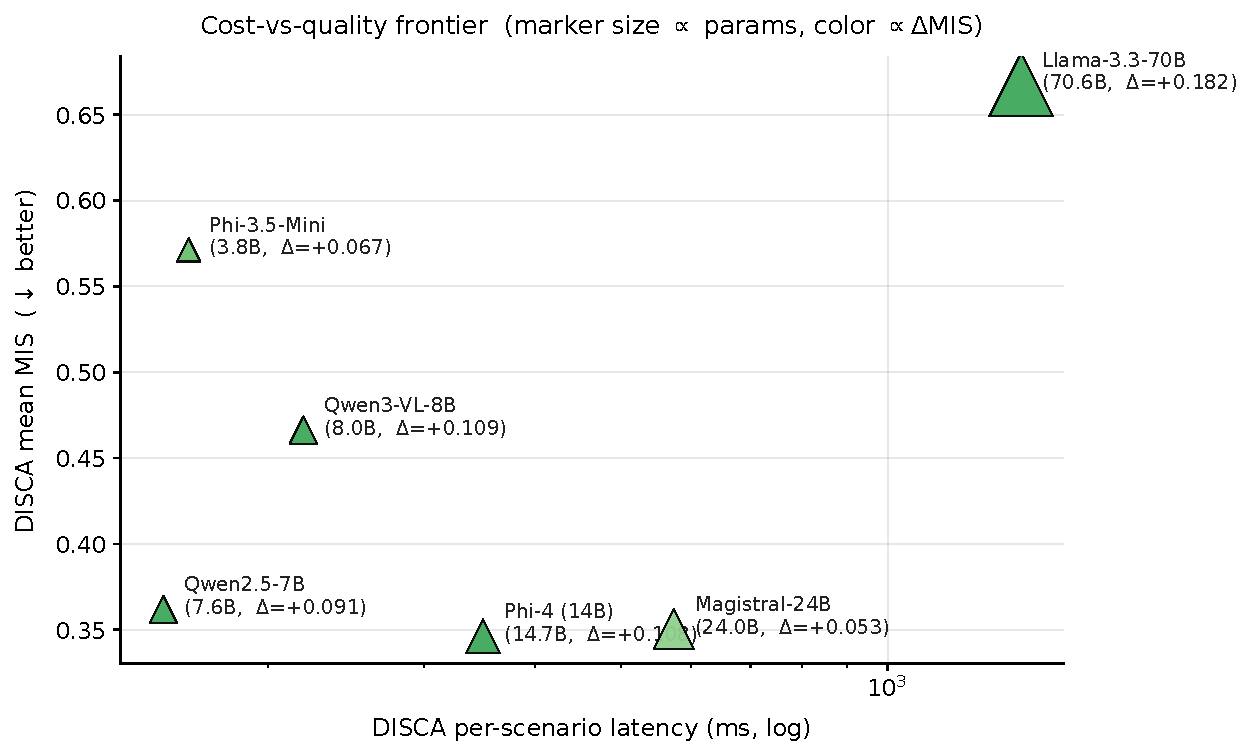
\includegraphics[width=0.9\linewidth]{latency_vs_mis.pdf}
  \caption{\textbf{Cost-vs-quality frontier on the headline 7 models.} Per-
  scenario DISCA latency (log scale) vs.\ mean DISCA MIS. Marker size is
  proportional to parameter count; color encodes $\Delta\mathrm{MIS}$ (greener
  = larger DISCA gain). Phi-4 (14B, $\Delta=+0.108$) lies bottom-left:
  Pareto-dominant over Llama-3.3-70B in both latency and alignment.}
  \label{fig:latency_vs_mis}
\end{figure}

\section{Engineering Journey: Method Selection}
\label{app:engineering}

DISCA (the ``EXP-24'' configuration) was selected from \textbf{25 method
variants} developed and evaluated on a fixed three-model, five-country prototyping
panel (Qwen2.5-7B, Gemma-2-9B, Mistral-7B $\times$ USA, CHN, JPN, DEU, BRA).
Table~\ref{tab:engineering} summarises the top-performing variants.

\begin{table}[H]\centering\scriptsize
\caption{Method variant comparison on the 3-model $\times$ 5-country prototyping
panel (15 rows). Mean MIS $\downarrow$. All variants share the same persona
construction and debiasing; they differ in IS-stage design.}
\label{tab:engineering}
\setlength{\tabcolsep}{4pt}
\begin{tabular}{clcc}\toprule
Rank & Method variant & Mean MIS $\downarrow$ & Key innovation \\\midrule
1 & EXP-23: Category-Coherence Reg. & 0.3956 & Blend IS toward per-cat mean \\
2 & \textbf{EXP-24: Dual-Pass Bootstrap (DPBR)} & \textbf{0.3969} & Soft $r{=}\exp(-v_b/s)$ reliability \\
3 & EXP-09: Hierarchical IS & 0.3975 & Cross-scenario smoothing (legacy) \\
4 & EXP-22: Adaptive IS $\sigma$ & 0.3977 & $\sigma$ from agent/history stats \\
5 & EXP-16: Nesterov IS & 0.3977 & Momentum + progressive PT \\
6 & EXP-17: Dual-Momentum Prior & 0.3979 & Fast/slow $\beta$ EMA blend \\
7 & EXP-10: Grand Fusion & 0.3982 & EXP-03+05+09 combined \\
\midrule
18 & EXP-01: Base SWA-PTIS & 0.4269 & Single-pass IS baseline \\
25 & EXP-12: Contrastive Personas & 0.4517 & World-average subtraction \\
\bottomrule
\end{tabular}
\end{table}

The top cluster (ranks 1--7) is separated by only 0.0026 MIS, but DPBR was
selected over the marginally-better EXP-23 for two reasons:
(i)~DPBR materially \textbf{lowers flip rate} (the fraction of scenarios where IS
reverses the consensus decision) compared to all other top-cluster methods,
improving deployment stability; and
(ii)~the dual-pass bootstrap provides an \textbf{interpretable uncertainty signal}
($r$ in Eq.~\ref{eq:dpbr_rel}) that can be logged and audited per scenario.
The base SWA-PTIS (rank~18) shows the value added by the dual-pass
stabilization stages: a 7\% relative MIS improvement.
Contrastive persona decoding (rank~25) \emph{hurts} alignment, validating the
design choice discussed in \S\ref{sec:related} to use direct WVS personas
rather than contrastive amplification.

% ============================================================================
\section{Relationship to Persona-Dependent LLM Alignment}
\label{app:kim_comparison}
% ============================================================================

\citet{kim2025persona} is the closest prior work to DISCA in studying persona effects on LLM moral decisions. Their study and ours share the Moral Machine framework and AMCE-based evaluation, but differ fundamentally in goal, method, and scope. Table~\ref{tab:kim_comparison} summarises the key distinctions.

\begin{table}[H]\centering\small
\caption{Comparison between \citet{kim2025persona} and DISCA.}
\label{tab:kim_comparison}
\setlength{\tabcolsep}{4pt}
\begin{tabular}{lll}\toprule
Dimension & Kim et al.\ (2025) & DISCA (this work) \\\midrule
Goal & Measure persona sensitivity & Correct cultural misalignment \\
Personas & 7 sociodemographic categories & 4 WVS-grounded agents per country \\
Persona source & Author-designed binary labels & Empirical WVS-7 microdata \\
Metric & MDD (persona-pair distance) & MIS ($\ell_2$ to human AMCE) \\
Correction & None (diagnostic only) & PT-IS + dual-pass reliability gate \\
Models & 3 (GPT-4o, GPT-3.5, Llama-2) & 7 checkpoints, 5 families, 2B--70B \\
Countries & Aggregate (Western vs.\ Eastern) & 20 individual countries \\
Scenarios & 9 dimensions, 10k synthetic & 6 dimensions, 310--500 per country \\
Theory & Partisan sorting (descriptive) & James--Stein shrinkage (Thm.~\ref{thm:shrinkage}) \\
\bottomrule
\end{tabular}
\end{table}

Three findings from \citet{kim2025persona} directly inform DISCA's design.

\paragraph{Persona sensitivity motivates disagreement-driven steering.} Kim et al.\ show that LLMs exhibit moral-decision distances (MDD) 2--4$\times$ larger than humans under contrasting personas. This confirms that persona prompts do shift LLM moral reasoning substantially, validating the premise that within-country persona spread is an informative signal. DISCA converts this sensitivity from a liability (uncontrolled decision shifts) into a feature (a sufficient statistic for correction reliability, Theorem~\ref{thm:shrinkage}).

\paragraph{The partisan sorting phenomenon justifies WVS grounding.} Kim et al.\ find that political orientation produces the largest persona effect in LLMs, far exceeding its effect in human respondents. This ``partisan sorting'' effect reveals that LLMs over-index on politically salient dimensions when given sociodemographic labels. DISCA avoids this pathology by grounding personas in empirical WVS-7 microdata rather than author-designed binary labels: the ten-dimensional cultural profile (Table~\ref{tab:wvs_thresholds}) distributes influence across religiosity, child-rearing values, social trust, and other axes, preventing any single dimension from dominating the correction. The leave-one-WVS-dim-out probe (Table~\ref{tab:wvs_impact_matrix}) confirms that influence is distributed rather than concentrated.

\paragraph{Moral flips validate the reliability gate.} Kim et al.\ document that specific personas can entirely reverse LLM preferences on certain moral dimensions (e.g., social status under a progressive persona in GPT-4o). DISCA's dual-pass reliability gate (Eq.~\ref{eq:dpbr_rel}) is designed precisely for this regime: when persona-driven corrections are large enough to flip the decision, the two independent IS passes are likely to disagree, and the exponential decay weight $r$ shrinks the correction toward zero. The tail-safety analysis (Table~\ref{tab:tail_safety}) confirms this mechanism reduces harmed cells from 11/120 to 3/120 compared to ungated consensus.

\paragraph{From diagnosis to correction.} The fundamental advance of DISCA over the Kim et al.\ framework is operational: where they diagnose persona sensitivity, we harness it. Their MDD metric measures the distance between two contrasting personas; our MIS measures the distance to the human target and actively reduces it. The James--Stein result (Theorem~\ref{thm:shrinkage}) provides the formal bridge: within-panel disagreement (analogous to their MDD) is a sufficient statistic for the correction's reliability, and the shrinkage estimator converts this diagnostic signal into an optimal correction.

% ============================================================================
\section{Extended Limitations}
\label{app:limitations}

This appendix expands the limitations summarised in §\ref{sec:discussion} with technical caveats not covered in the main text.

\paragraph{WVS-to-trolley linkage.}
The mapping from WVS value dimensions to trolley moral dimensions operates through both direct thematic overlap and indirect modulation (Appendix~\ref{app:wvs_linkage}). The 10-dimensional WVS profile explains $R^2 \in [0.55, 0.69]$ of human AMCE variance, and a leave-one-dimension-out probe identifies load-bearing couplings alongside noisy ones that the IS stage automatically down-weights. We avoid claims of the form ``WVS dimension $X$ caused AMCE shift $Y$,'' but the ensemble design and the IS noise-filtering mechanism together ensure the method is robust even when individual WVS--trolley links are imperfect.

\paragraph{Inter-persona reward assumption.}
The reward $r_i = \delta_i - \delta_{\text{base}}$ assumes persona shifts approximate human target directions. This is plausible when the base model represents a WEIRD-biased prior, but if a persona's shift is orthogonal to the human target, the signal may mislead. Quantifying whether persona-consensus directions correlate with country-level human AMCE vectors independently of the base model-and when corrections diverge from targets-is open; we do not report that correlation matrix here.

\paragraph{Geographic coverage, preprocessing, and WVS vintage.}
We report 20 countries out of 100+ MultiTP countries; results depend on the preprocessing pipeline in Appendix~\ref{app:dataset_sens}. WVS Wave~7 ($\sim$2017--2022) is a fixed historical slice that may not reflect current preferences in rapidly evolving societies; persona quality is weakest where coverage is sparse (e.g., Saudi Arabia, Brazil), as reflected in per-country tables. No low-resource languages (Amharic, Khmer, Yoruba) appear in the panel; cross-lingual generalisation to such settings remains untested, and one language per country may conflate linguistic and cultural effects.

\paragraph{Model quantisation.}
4-bit/Int8 quantisation may introduce logit artefacts affecting IS stability-observed empirically on Unsloth Phi-4 prior to switching to vLLM BF16 for the headline runs.


% ============================================================
% NeurIPS checklist (must appear with submission)
% ============================================================
\newpage
\section*{NeurIPS Paper Checklist}

%%% BEGIN INSTRUCTIONS %%%
The checklist is designed to encourage best practices for responsible machine learning research, addressing issues of reproducibility, transparency, research ethics, and societal impact. Do not remove the checklist: {\bf The papers not including the checklist will be desk rejected.} The checklist should follow the references and follow the (optional) supplemental material.  The checklist does NOT count towards the page
limit. 

Please read the checklist guidelines carefully for information on how to answer these questions. For each question in the checklist:
\begin{itemize}
    \item You should answer \answerYes{}, \answerNo{}, or \answerNA{}.
    \item \answerNA{} means either that the question is Not Applicable for that particular paper or the relevant information is Not Available.
    \item Please provide a short (1--2 sentence) justification right after your answer (even for \answerNA). 
   % \item {\bf The papers not including the checklist will be desk rejected.}
\end{itemize}

{\bf The checklist answers are an integral part of your paper submission.} They are visible to the reviewers, area chairs, senior area chairs, and ethics reviewers. You will also be asked to include it (after eventual revisions) with the final version of your paper, and its final version will be published with the paper.

The reviewers of your paper will be asked to use the checklist as one of the factors in their evaluation. While \answerYes{} is generally preferable to \answerNo{}, it is perfectly acceptable to answer \answerNo{} provided a proper justification is given (e.g., error bars are not reported because it would be too computationally expensive'' or ``we were unable to find the license for the dataset we used''). In general, answering \answerNo{} or \answerNA{} is not grounds for rejection. While the questions are phrased in a binary way, we acknowledge that the true answer is often more nuanced, so please just use your best judgment and write a justification to elaborate. All supporting evidence can appear either in the main paper or the supplemental material, provided in appendix. If you answer \answerYes{} to a question, in the justification please point to the section(s) where related material for the question can be found.

IMPORTANT, please:
\begin{itemize}
    \item {\bf Delete this instruction block, but keep the section heading ``NeurIPS Paper Checklist"},
    \item  {\bf Keep the checklist subsection headings, questions/answers and guidelines below.}
    \item {\bf Do not modify the questions and only use the provided macros for your answers}.
\end{itemize} 
 

%%% END INSTRUCTIONS %%%


\begin{enumerate}

\item {\bf Claims}
    \item[] Question: Do the main claims made in the abstract and introduction accurately reflect the paper's contributions and scope?
    \item[] Answer: \answerYes{}
    \item[] Justification: The abstract and \S\ref{sec:intro} state three claims: (i) DISCA is a train-free inference-time controller that requires no per-country reward models or extra training data; (ii) it cuts macro MIS by 10--24\% on seven open-weight backbones across 20 countries and 6 moral dimensions; (iii) calibration competes with scale (Phi-4 14B beats Llama-3.3-70B in absolute MIS). All three are substantiated in Table~\ref{tab:main_macro_summary} and Figure~\ref{fig:scaling_vs_calibration}; scope and assumptions (binary dilemmas with decision-token logits, WVS-7 vintage) are made explicit in \S\ref{sec:discussion} and Appendix~\ref{app:limitations}.
    \item[] Guidelines:
    \begin{itemize}
        \item The answer \answerNA{} means that the abstract and introduction do not include the claims made in the paper.
        \item The abstract and/or introduction should clearly state the claims made, including the contributions made in the paper and important assumptions and limitations. A \answerNo{} or \answerNA{} answer to this question will not be perceived well by the reviewers. 
        \item The claims made should match theoretical and experimental results, and reflect how much the results can be expected to generalize to other settings. 
        \item It is fine to include aspirational goals as motivation as long as it is clear that these goals are not attained by the paper. 
    \end{itemize}

\item {\bf Limitations}
    \item[] Question: Does the paper discuss the limitations of the work performed by the authors?
    \item[] Answer: \answerYes{}
    \item[] Justification: \S\ref{sec:discussion} bounds generalisation with three caveats (alignment to a survey statistic vs.\ perceived legitimacy; PT value function as aggregation kernel rather than cognitive model; decision-token logit requirement). Appendix~\ref{app:limitations} expands these with: WVS-to-trolley linkage being indirect, the inter-persona reward assumption, geographic coverage (20 of 100+ MultiTP countries; sparse personas for under-sampled countries), WVS Wave~7 vintage, and 4-bit/Int8 quantisation artefacts on IS stability.
    \item[] Guidelines:
    \begin{itemize}
        \item The answer \answerNA{} means that the paper has no limitation while the answer \answerNo{} means that the paper has limitations, but those are not discussed in the paper. 
        \item The authors are encouraged to create a separate ``Limitations'' section in their paper.
        \item The paper should point out any strong assumptions and how robust the results are to violations of these assumptions (e.g., independence assumptions, noiseless settings, model well-specification, asymptotic approximations only holding locally). The authors should reflect on how these assumptions might be violated in practice and what the implications would be.
        \item The authors should reflect on the scope of the claims made, e.g., if the approach was only tested on a few datasets or with a few runs. In general, empirical results often depend on implicit assumptions, which should be articulated.
        \item The authors should reflect on the factors that influence the performance of the approach. For example, a facial recognition algorithm may perform poorly when image resolution is low or images are taken in low lighting. Or a speech-to-text system might not be used reliably to provide closed captions for online lectures because it fails to handle technical jargon.
        \item The authors should discuss the computational efficiency of the proposed algorithms and how they scale with dataset size.
        \item If applicable, the authors should discuss possible limitations of their approach to address problems of privacy and fairness.
        \item While the authors might fear that complete honesty about limitations might be used by reviewers as grounds for rejection, a worse outcome might be that reviewers discover limitations that aren't acknowledged in the paper. The authors should use their best judgment and recognize that individual actions in favor of transparency play an important role in developing norms that preserve the integrity of the community. Reviewers will be specifically instructed to not penalize honesty concerning limitations.
    \end{itemize}

\item {\bf Theory assumptions and proofs}
    \item[] Question: For each theoretical result, does the paper provide the full set of assumptions and a complete (and correct) proof?
    \item[] Answer: \answerYes{}
    \item[] Justification: The single theoretical result, Theorem~\ref{thm:shrinkage} (minimax-optimality of disagreement-driven shrinkage in the James--Stein sense for panels of $N\geq 4$), is stated in the main text with all assumptions (panel size, Gaussian persona shifts, $\ell_2$ risk). The full proof, including referenced lemmas, is given in Appendix~\ref{app:bias_variance}. A short proof sketch and the connection to Eq.~\ref{eq:util_total} appear in \S\ref{sec:method}.
    \item[] Guidelines:
    \begin{itemize}
        \item The answer \answerNA{} means that the paper does not include theoretical results. 
        \item All the theorems, formulas, and proofs in the paper should be numbered and cross-referenced.
        \item All assumptions should be clearly stated or referenced in the statement of any theorems.
        \item The proofs can either appear in the main paper or the supplemental material, but if they appear in the supplemental material, the authors are encouraged to provide a short proof sketch to provide intuition. 
        \item Inversely, any informal proof provided in the core of the paper should be complemented by formal proofs provided in appendix or supplemental material.
        \item Theorems and Lemmas that the proof relies upon should be properly referenced. 
    \end{itemize}

    \item {\bf Experimental result reproducibility}
    \item[] Question: Does the paper fully disclose all the information needed to reproduce the main experimental results of the paper to the extent that it affects the main claims and/or conclusions of the paper (regardless of whether the code and data are provided or not)?
    \item[] Answer: \answerYes{}
    \item[] Justification: \S\ref{sec:method} gives the full algorithm (Algorithm~1, Eqs.~\ref{eq:util_total}--\ref{eq:disca_rel}); the full hyperparameter table (Table~\ref{tab:hyperparams}) lists every numerical default with the validation procedure (synthetic 200-scenario pool, transferability check on a 50-scenario MultiTP English subset). All backbones are publicly available open-weight checkpoints. Preprocessing (cap=80, oversample=36), seeds (3), and per-country preprocessing details are documented in Appendices~\ref{app:dataset_sens},~\ref{sec:multiseed}. We additionally release a self-contained reference implementation (\texttt{DISCA\_Alignment/}) with the same defaults and a single-command sweep entry point.
    \item[] Guidelines:
    \begin{itemize}
        \item The answer \answerNA{} means that the paper does not include experiments.
        \item If the paper includes experiments, a \answerNo{} answer to this question will not be perceived well by the reviewers: Making the paper reproducible is important, regardless of whether the code and data are provided or not.
        \item If the contribution is a dataset and\slash or model, the authors should describe the steps taken to make their results reproducible or verifiable. 
        \item Depending on the contribution, reproducibility can be accomplished in various ways. For example, if the contribution is a novel architecture, describing the architecture fully might suffice, or if the contribution is a specific model and empirical evaluation, it may be necessary to either make it possible for others to replicate the model with the same dataset, or provide access to the model. In general. releasing code and data is often one good way to accomplish this, but reproducibility can also be provided via detailed instructions for how to replicate the results, access to a hosted model (e.g., in the case of a large language model), releasing of a model checkpoint, or other means that are appropriate to the research performed.
        \item While NeurIPS does not require releasing code, the conference does require all submissions to provide some reasonable avenue for reproducibility, which may depend on the nature of the contribution. For example
        \begin{enumerate}
            \item If the contribution is primarily a new algorithm, the paper should make it clear how to reproduce that algorithm.
            \item If the contribution is primarily a new model architecture, the paper should describe the architecture clearly and fully.
            \item If the contribution is a new model (e.g., a large language model), then there should either be a way to access this model for reproducing the results or a way to reproduce the model (e.g., with an open-source dataset or instructions for how to construct the dataset).
            \item We recognize that reproducibility may be tricky in some cases, in which case authors are welcome to describe the particular way they provide for reproducibility. In the case of closed-source models, it may be that access to the model is limited in some way (e.g., to registered users), but it should be possible for other researchers to have some path to reproducing or verifying the results.
        \end{enumerate}
    \end{itemize}


\item {\bf Open access to data and code}
    \item[] Question: Does the paper provide open access to the data and code, with sufficient instructions to faithfully reproduce the main experimental results, as described in supplemental material?
    \item[] Answer: \answerYes{}
    \item[] Justification: We release \texttt{DISCA\_Alignment/} (anonymised for review; MIT-licensed) as supplemental material. The package is a self-contained slice of the research codebase: a single CLI entry point (\texttt{run.py}) drives the per-model 20-country sweep, with backend selection (\texttt{vllm} / \texttt{hf\_native} / \texttt{unsloth}) and explicit flags for the three external data paths (\texttt{--multitp-data}, \texttt{--wvs-data}, \texttt{--human-amce}). The README documents install (Python 3.10+, CUDA 12.x), HF token wiring for gated models, exact commands, and the output schema (per-country baseline / DISCA CSVs and a comparison file). MultiTP, WVS-7 Wave, and the human AMCE table are publicly available datasets cited in \S\ref{sec:exp:data}; access instructions are reproduced in the README.
    \item[] Guidelines:
    \begin{itemize}
        \item The answer \answerNA{} means that paper does not include experiments requiring code.
        \item Please see the NeurIPS code and data submission guidelines (\url{https://neurips.cc/public/guides/CodeSubmissionPolicy}) for more details.
        \item While we encourage the release of code and data, we understand that this might not be possible, so \answerNo{} is an acceptable answer. Papers cannot be rejected simply for not including code, unless this is central to the contribution (e.g., for a new open-source benchmark).
        \item The instructions should contain the exact command and environment needed to run to reproduce the results. See the NeurIPS code and data submission guidelines (\url{https://neurips.cc/public/guides/CodeSubmissionPolicy}) for more details.
        \item The authors should provide instructions on data access and preparation, including how to access the raw data, preprocessed data, intermediate data, and generated data, etc.
        \item The authors should provide scripts to reproduce all experimental results for the new proposed method and baselines. If only a subset of experiments are reproducible, they should state which ones are omitted from the script and why.
        \item At submission time, to preserve anonymity, the authors should release anonymized versions (if applicable).
        \item Providing as much information as possible in supplemental material (appended to the paper) is recommended, but including URLs to data and code is permitted.
    \end{itemize}


\item {\bf Experimental setting/details}
    \item[] Question: Does the paper specify all the training and test details (e.g., data splits, hyperparameters, how they were chosen, type of optimizer) necessary to understand the results?
    \item[] Answer: \answerYes{}
    \item[] Justification: There is no training (the method is inference-time on frozen weights); we therefore detail all decoding and controller settings. \S\ref{sec:experiments} specifies the dataset (MultiTP, 20 countries), preprocessing (deduplication, category cap=80, oversample to $\geq$36 per dimension), the seven main backbones with sizes, and the metric definitions (MIS, Pearson $r$, JSD, win rate). All hyperparameters and how they were chosen are tabulated in Table~\ref{tab:hyperparams} with the synthetic-pool grid-search procedure described in Appendix~\ref{app:hyperparams}. Sensitivity sweeps for the temperature family (Appendix~\ref{app:temp_sensitivity}), category cap (Appendix~\ref{app:r2_oversampling}), and the controller knobs ($s$, $\lambda_{\text{coop}}$, $\sigma$, $T_{\text{cat}}$) appear in Appendix~\ref{app:hyperparams}.
    \item[] Guidelines:
    \begin{itemize}
        \item The answer \answerNA{} means that the paper does not include experiments.
        \item The experimental setting should be presented in the core of the paper to a level of detail that is necessary to appreciate the results and make sense of them.
        \item The full details can be provided either with the code, in appendix, or as supplemental material.
    \end{itemize}

\item {\bf Experiment statistical significance}
    \item[] Question: Does the paper report error bars suitably and correctly defined or other appropriate information about the statistical significance of the experiments?
    \item[] Answer: \answerYes{}
    \item[] Justification: The headline table (Table~\ref{tab:main_macro_summary}) reports macro MIS as mean $\pm$ standard deviation across 3 independent seeds (independent IS noise draws; the underlying model weights and data are fixed). A separate multi-seed stability analysis (Appendix~\ref{sec:multiseed}) gives per-country variability, and a bootstrap confidence interval on JSD ($\pm 0.004$, Appendix~\ref{app:robustness_summary}) quantifies the noise floor for distributional metrics. We explicitly state that conclusions are stable well within the bootstrap noise floor; sensitivity sweeps along nine independent axes confirm this.
    \item[] Guidelines:
    \begin{itemize}
        \item The answer \answerNA{} means that the paper does not include experiments.
        \item The authors should answer \answerYes{} if the results are accompanied by error bars, confidence intervals, or statistical significance tests, at least for the experiments that support the main claims of the paper.
        \item The factors of variability that the error bars are capturing should be clearly stated (for example, train/test split, initialization, random drawing of some parameter, or overall run with given experimental conditions).
        \item The method for calculating the error bars should be explained (closed form formula, call to a library function, bootstrap, etc.)
        \item The assumptions made should be given (e.g., Normally distributed errors).
        \item It should be clear whether the error bar is the standard deviation or the standard error of the mean.
        \item It is OK to report 1-sigma error bars, but one should state it. The authors should preferably report a 2-sigma error bar than state that they have a 96\% CI, if the hypothesis of Normality of errors is not verified.
        \item For asymmetric distributions, the authors should be careful not to show in tables or figures symmetric error bars that would yield results that are out of range (e.g., negative error rates).
        \item If error bars are reported in tables or plots, the authors should explain in the text how they were calculated and reference the corresponding figures or tables in the text.
    \end{itemize}

\item {\bf Experiments compute resources}
    \item[] Question: For each experiment, does the paper provide sufficient information on the computer resources (type of compute workers, memory, time of execution) needed to reproduce the experiments?
    \item[] Answer: \answerYes{}
    \item[] Justification: Appendix~\ref{app:trigger} (Table~\ref{tab:r2_latency_compact}) reports per-scenario wall-clock on a single H100 GPU: 0.083--0.086 s/scenario for DISCA at $K\in\{64,128,256\}$ vs.\ 0.023 s/scenario for vanilla decoding (3.57--3.72$\times$ overhead). Backbone-level cost is given in Figure~\ref{fig:latency_vs_mis}: 350~ms/scenario for Phi-4 vs.\ 1414~ms for Llama-3.3-70B with DISCA. Sub-70B backbones run on a single H100 in BF16 via vLLM; the 70B backbone uses 4-bit Unsloth on the same hardware. The released code's CLI also runs end-to-end on a Kaggle T4/P100 dual-GPU node for sub-14B models. We acknowledge in Appendix~\ref{app:engineering} that exploratory experiments (25 controller variants on a 3-backbone $\times$ 5-country prototyping panel) consumed substantially more compute than the reported runs.
    \item[] Guidelines:
    \begin{itemize}
        \item The answer \answerNA{} means that the paper does not include experiments.
        \item The paper should indicate the type of compute workers CPU or GPU, internal cluster, or cloud provider, including relevant memory and storage.
        \item The paper should provide the amount of compute required for each of the individual experimental runs as well as estimate the total compute. 
        \item The paper should disclose whether the full research project required more compute than the experiments reported in the paper (e.g., preliminary or failed experiments that didn't make it into the paper). 
    \end{itemize}
    
\item {\bf Code of ethics}
    \item[] Question: Does the research conducted in the paper conform, in every respect, with the NeurIPS Code of Ethics \url{https://neurips.cc/public/EthicsGuidelines}?
    \item[] Answer: \answerYes{}
    \item[] Justification: The authors have reviewed the NeurIPS Code of Ethics. The work uses only public, ethically-collected datasets (MultiTP~\citep{jin2025multitp}, World Values Survey Wave~7, Moral Machine human AMCEs~\citep{awad2018moral}); it conducts no new human-subjects research and introduces no scraped data. Anonymity is preserved in the submission. Negative-impact considerations (risk of encoding harmful majorities) are explicitly discussed in \S\ref{sec:discussion} with a per-persona utility floor mitigation validated in Appendix~\ref{app:hyperparams} (Table~\ref{tab:r2_persona_floor}).
    \item[] Guidelines:
    \begin{itemize}
        \item The answer \answerNA{} means that the authors have not reviewed the NeurIPS Code of Ethics.
        \item If the authors answer \answerNo, they should explain the special circumstances that require a deviation from the Code of Ethics.
        \item The authors should make sure to preserve anonymity (e.g., if there is a special consideration due to laws or regulations in their jurisdiction).
    \end{itemize}


\item {\bf Broader impacts}
    \item[] Question: Does the paper discuss both potential positive societal impacts and negative societal impacts of the work performed?
    \item[] Answer: \answerYes{}
    \item[] Justification: \S\ref{sec:discussion} discusses both directions. Positive: a train-free, low-overhead controller lets practitioners respect cross-national preference heterogeneity at deployment time without finetuning per country, lowering the barrier to culturally pluralistic alignment. Negative: aligning to majority survey statistics could entrench harmful majorities or marginalise minority views~\citep{zewail2025moral}, and alignment to a survey statistic is not equivalent to legitimacy~\citep{atari2023humans}. We propose and validate a per-persona utility floor that caps how far any single persona's post-correction utility can drop from vanilla (Appendix~\ref{app:hyperparams}, Table~\ref{tab:r2_persona_floor}), and we are explicit that DISCA is a research artefact, not a deployment-ready normative system.
    \item[] Guidelines:
    \begin{itemize}
        \item The answer \answerNA{} means that there is no societal impact of the work performed.
        \item If the authors answer \answerNA{} or \answerNo, they should explain why their work has no societal impact or why the paper does not address societal impact.
        \item Examples of negative societal impacts include potential malicious or unintended uses (e.g., disinformation, generating fake profiles, surveillance), fairness considerations (e.g., deployment of technologies that could make decisions that unfairly impact specific groups), privacy considerations, and security considerations.
        \item The conference expects that many papers will be foundational research and not tied to particular applications, let alone deployments. However, if there is a direct path to any negative applications, the authors should point it out. For example, it is legitimate to point out that an improvement in the quality of generative models could be used to generate Deepfakes for disinformation. On the other hand, it is not needed to point out that a generic algorithm for optimizing neural networks could enable people to train models that generate Deepfakes faster.
        \item The authors should consider possible harms that could arise when the technology is being used as intended and functioning correctly, harms that could arise when the technology is being used as intended but gives incorrect results, and harms following from (intentional or unintentional) misuse of the technology.
        \item If there are negative societal impacts, the authors could also discuss possible mitigation strategies (e.g., gated release of models, providing defenses in addition to attacks, mechanisms for monitoring misuse, mechanisms to monitor how a system learns from feedback over time, improving the efficiency and accessibility of ML).
    \end{itemize}
    
\item {\bf Safeguards}
    \item[] Question: Does the paper describe safeguards that have been put in place for responsible release of data or models that have a high risk for misuse (e.g., pre-trained language models, image generators, or scraped datasets)?
    \item[] Answer: \answerNA{}
    \item[] Justification: We do not release any pretrained models, generative models, or scraped datasets. The released artefact (\texttt{DISCA\_Alignment/}) is an inference-time controller layered over publicly available open-weight LLMs whose existing safeguards remain in place. The method itself produces no novel generative capability beyond that of the underlying models; the per-persona utility floor (Appendix~\ref{app:hyperparams}, Table~\ref{tab:r2_persona_floor}) is included as an in-method safeguard against majoritarian skew.
    \item[] Guidelines:
    \begin{itemize}
        \item The answer \answerNA{} means that the paper poses no such risks.
        \item Released models that have a high risk for misuse or dual-use should be released with necessary safeguards to allow for controlled use of the model, for example by requiring that users adhere to usage guidelines or restrictions to access the model or implementing safety filters. 
        \item Datasets that have been scraped from the Internet could pose safety risks. The authors should describe how they avoided releasing unsafe images.
        \item We recognize that providing effective safeguards is challenging, and many papers do not require this, but we encourage authors to take this into account and make a best faith effort.
    \end{itemize}

\item {\bf Licenses for existing assets}
    \item[] Question: Are the creators or original owners of assets (e.g., code, data, models), used in the paper, properly credited and are the license and terms of use explicitly mentioned and properly respected?
    \item[] Answer: \answerYes{}
    \item[] Justification: All third-party assets are cited with version information. Datasets: MultiTP~\citep{jin2025multitp}, the Moral Machine human AMCE table~\citep{awad2018moral}, and World Values Survey Wave~7 (\texttt{WVS\_Cross-National\_Wave\_7\_inverted\_csv\_v6\_0.csv}) are used under the terms of the respective public releases. Models: Phi-4 and Phi-3.5-mini (MIT), Llama-3.3-70B (Llama-3 Community License), Qwen-2.5/3-VL (Apache-2.0/Qwen license), Gemma family (Gemma terms of use), Magistral-Small-2509 (Apache-2.0). Code dependencies (Transformers, vLLM, Unsloth, bitsandbytes) are listed with version pins in the released \texttt{requirements.txt}; we use them under their stated licenses (mostly Apache-2.0/MIT). The \texttt{compute\_ACME} reference implementation we follow is credited to~\citet{jin2025multitp} in Appendix~\ref{app:amce}.
    \item[] Guidelines:
    \begin{itemize}
        \item The answer \answerNA{} means that the paper does not use existing assets.
        \item The authors should cite the original paper that produced the code package or dataset.
        \item The authors should state which version of the asset is used and, if possible, include a URL.
        \item The name of the license (e.g., CC-BY 4.0) should be included for each asset.
        \item For scraped data from a particular source (e.g., website), the copyright and terms of service of that source should be provided.
        \item If assets are released, the license, copyright information, and terms of use in the package should be provided. For popular datasets, \url{paperswithcode.com/datasets} has curated licenses for some datasets. Their licensing guide can help determine the license of a dataset.
        \item For existing datasets that are re-packaged, both the original license and the license of the derived asset (if it has changed) should be provided.
        \item If this information is not available online, the authors are encouraged to reach out to the asset's creators.
    \end{itemize}

\item {\bf New assets}
    \item[] Question: Are new assets introduced in the paper well documented and is the documentation provided alongside the assets?
    \item[] Answer: \answerYes{}
    \item[] Justification: We release the DISCA reference implementation (\texttt{DISCA\_Alignment/}) as a new code asset under the MIT License. The package ships with: a top-level README documenting installation, backend selection (vLLM / HF native / Unsloth), the three external data flags, environment variables, the quick-start command, and the output schema; a flat \texttt{disca/} module with one-purpose files (controller, dual-pass core, runner, AMCE/metrics, persona generation, multilingual scenarios, model loader); pinned dependencies in \texttt{requirements.txt}; and a single CLI entry point (\texttt{run.py --help}). The submission archive is anonymised. All hyperparameter defaults match Table~\ref{tab:hyperparams} in the main paper.
    \item[] Guidelines:
    \begin{itemize}
        \item The answer \answerNA{} means that the paper does not release new assets.
        \item Researchers should communicate the details of the dataset\slash code\slash model as part of their submissions via structured templates. This includes details about training, license, limitations, etc. 
        \item The paper should discuss whether and how consent was obtained from people whose asset is used.
        \item At submission time, remember to anonymize your assets (if applicable). You can either create an anonymized URL or include an anonymized zip file.
    \end{itemize}

\item {\bf Crowdsourcing and research with human subjects}
    \item[] Question: For crowdsourcing experiments and research with human subjects, does the paper include the full text of instructions given to participants and screenshots, if applicable, as well as details about compensation (if any)?
    \item[] Answer: \answerNA{}
    \item[] Justification: The paper conducts no new crowdsourcing or human-subjects research. Human reference data is reused from the existing public Moral Machine experiment~\citep{awad2018moral} as packaged by MultiTP~\citep{jin2025multitp}, and from the World Values Survey Wave~7 public microdata; we make no new contact with participants and recruit no annotators.
    \item[] Guidelines:
    \begin{itemize}
        \item The answer \answerNA{} means that the paper does not involve crowdsourcing nor research with human subjects.
        \item Including this information in the supplemental material is fine, but if the main contribution of the paper involves human subjects, then as much detail as possible should be included in the main paper. 
        \item According to the NeurIPS Code of Ethics, workers involved in data collection, curation, or other labor should be paid at least the minimum wage in the country of the data collector. 
    \end{itemize}

\item {\bf Institutional review board (IRB) approvals or equivalent for research with human subjects}
    \item[] Question: Does the paper describe potential risks incurred by study participants, whether such risks were disclosed to the subjects, and whether Institutional Review Board (IRB) approvals (or an equivalent approval/review based on the requirements of your country or institution) were obtained?
    \item[] Answer: \answerNA{}
    \item[] Justification: No new human-subjects research is conducted. The work is a secondary analysis of pre-existing public datasets (Moral Machine human AMCEs, MultiTP scenarios, WVS-7 microdata), each of which carries its own ethics review at the original collection point; no further IRB approval applies.
    \item[] Guidelines:
    \begin{itemize}
        \item The answer \answerNA{} means that the paper does not involve crowdsourcing nor research with human subjects.
        \item Depending on the country in which research is conducted, IRB approval (or equivalent) may be required for any human subjects research. If you obtained IRB approval, you should clearly state this in the paper. 
        \item We recognize that the procedures for this may vary significantly between institutions and locations, and we expect authors to adhere to the NeurIPS Code of Ethics and the guidelines for their institution. 
        \item For initial submissions, do not include any information that would break anonymity (if applicable), such as the institution conducting the review.
    \end{itemize}

\item {\bf Declaration of LLM usage}
    \item[] Question: Does the paper describe the usage of LLMs if it is an important, original, or non-standard component of the core methods in this research? Note that if the LLM is used only for writing, editing, or formatting purposes and does \emph{not} impact the core methodology, scientific rigor, or originality of the research, declaration is not required.
    %this research?
    \item[] Answer: \answerYes{}
    \item[] Justification: LLMs are central to the work in two ways, both fully described. (i) Frozen open-weight LLMs (Phi-4, Llama-3.3-70B, Magistral-24B, Qwen3-VL-8B, Qwen2.5-7B, Phi-3.5-mini, Gemma-4-E2B) are the \emph{subject} that DISCA steers; their identities, sizes, and decoding settings are documented in \S\ref{sec:exp:models} and Appendix~\ref{app:model_landscape}. (ii) For the open-ended extension (\S\ref{sec:method:openended}), an LLM parses free-form responses into a (choice, confidence) pair to recover a pseudo-logit-gap; this auxiliary use is documented in that section. A separate synthetic 200-scenario tuning pool generated by GPT-4 is disclosed in Appendix~\ref{app:hyperparams} along with its limitations. LLMs were not used to generate the paper's claims, results, or proofs.
    \item[] Guidelines:
    \begin{itemize}
        \item The answer \answerNA{} means that the core method development in this research does not involve LLMs as any important, original, or non-standard components.
        \item Please refer to our LLM policy in the NeurIPS handbook for what should or should not be described.
    \end{itemize}

\end{enumerate}


\end{document}
  